%%%%%%%%%%%%%%%%%%%%%%%%%%%%%%%%%%%%%%%%%
% UAThesis
% LaTeX Template
% Version 1.0 (01/09/15)
%
% Based on the template
%
% License:
% CC BY-NC-SA 3.0 (http://creativecommons.org/licenses/by-nc-sa/3.0/)
%
%%%%%%%%%%%%%%%%%%%%%%%%%%%%%%%%%%%%%%%%%

%----------------------------------------------------------------------------------------
%	PACKAGES AND OTHER DOCUMENT CONFIGURATIONS
%----------------------------------------------------------------------------------------

\documentclass[
  12pt,           % The default document font size, options: 10pt, 11pt, 12pt
  %oneside,       % Two side (alternating margins) for binding by default, uncomment to switch to one side
  english,        % Language option for the babel package
  onehalfspacing,  % Single line spacing, alternatives: onehalfspacing or doublespacing
  %draft,         % Uncomment to enable draft mode (no pictures, no links, overfull hboxes indicated)
  %nolistspacing, % If the document is onehalfspacing or doublespacing, uncomment this to set spacing in lists to single
  %liststotoc,    % Uncomment to add the list of figures/tables/etc to the table of contents
  %toctotoc,      % Uncomment to add the main table of contents to the table of contents
  %parskip,       % Uncomment to add space between paragraphs
]{UAThesis} % The class file specifying the document structure

%Cool numbers
%\usepackage{siunitx}

%Cool tables
\usepackage{array}
\usepackage{booktabs}
\usepackage{amssymb}
\usepackage{pifont}
\usepackage{threeparttable}
\usepackage{threeparttablex}
\usepackage{longtable}
\usepackage{pdflscape}

\newcolumntype{M}[1]{>{\centering\arraybackslash}m{#1}}
\newcommand{\ra}[1]{\renewcommand{\arraystretch}{#1}}
\newcommand{\0}{\mathord{\mspace{2mu}\star\mspace{2mu}}}
\newcommand{\tabitem}{~~\llap{\textbullet}~~}
\renewcommand{\tabcolsep}{5pt}
\newcommand{\xmark}{\ding{55}}

%Video Prediction taxonomy
\colorlet{linecol}{black!80}
\tikzset{
	my rounded corners/.append style={rounded corners=1pt},
}

\usepackage{textcomp}

%Subfigures and solving the problem of too large counter. labels after z: aa, ab...
\usepackage[caption=false]{subfig}
\usepackage{alphalph}
\renewcommand*{\thesubfigure}{%
	\alphalph{\value{subfigure}}%
}%

% Colors for unrealgrasp
\definecolor{azure}{rgb}{0.0, 0.5, 1.0}
\definecolor{red}{rgb}{0.93, 0.11, 0.14}
\definecolor{green}{rgb}{0.18, 0.55, 0.34}

%----------------------------------------------------------------------------------------
%	THESIS INFORMATION
%----------------------------------------------------------------------------------------

\thesistitle{Deep Predictive Learning:\\ TBD}
% Your thesis title, this is used in the title and abstract, print it elsewhere with \ttitle
\supervisor{Jose \textsc{Garcia-Rodriguez}}
% Your supervisor's name, this is used in the title page, print it elsewhere with \supname
\examiner{}
% Your examiner's name, this is not currently used anywhere in the template, print it elsewhere with \examname
\degree{Doctor of Philosophy}
% Your degree name, this is used in the title page and abstract, print it elsewhere with \degreename
\author{Sergiu-Ovidiu \textsc{Oprea}}
% Your name, this is used in the title page and abstract, print it elsewhere with \authorname
\addresses{} 
% Your address, this is not currently used anywhere in the template, print it elsewhere with \addressname
\subject{Computer Science}
% Your subject area, this is not currently used anywhere in the template, print it elsewhere with \subjectname
\keywords{}
% Keywords for your thesis, this is not currently used anywhere in the template, print it elsewhere with \keywordnames
\university{{University of Alicante}}
% Your university's name and URL, this is used in the title page and abstract, print it elsewhere with \univname
\department{{Department of Computer Technology}}
% Your department's name and URL, this is used in the title page and abstract, print it elsewhere with \deptname
\group{{3D Perception Lab}}
% Your research group's name and URL, this is used in the title page, print it elsewhere with \groupname
\faculty{\href{http://www.eps.ua.es/}{Higher Polytechnic School}}
% Your faculty's name and URL, this is used in the title page and abstract, print it elsewhere with \facname

\hypersetup{pdftitle=\ttitle} % Set the PDF's title to your title
\hypersetup{pdfauthor=\authorname} % Set the PDF's author to your name
\hypersetup{pdfkeywords=\keywordnames} % Set the PDF's keywords to your keywords

\begin{document}

\dominitoc

\frontmatter
% Use roman page numbering style (i, ii, iii, iv...) for the pre-content pages

\pagestyle{plain}
% Default to the plain heading style until the thesis style is called for the body content

%----------------------------------------------------------------------------------------
%	TITLE PAGE
%----------------------------------------------------------------------------------------

\begin{titlepage}
\begin{center}
	

\includegraphics[width=0.64\linewidth]{Figures/logoua}

\vfill

\textsc{\LARGE Departamento de Tecnología Informática y Computación}\\[1.5cm] % University name
\textsc{\Large Escuela Politécnica Superior}\\[0.5cm] % Thesis type

%\HRule \\[0.4cm] % Horizontal line
{\huge \bfseries \ttitle}\\[0.4cm] % Thesis title
%\HRule \\[1.5cm] % Horizontal line
 
\begin{center} \large
{\authorname} % Author name - remove the \href bracket to remove the link
\\\ \\
\emph{Tesis presentada para aspirar al grado de} \\
{DOCTOR POR LA UNIVERSIDAD DE ALICANTE}\\\
{MENCIÓN DE DOCTOR INTERNACIONAL}\\
{DOCTORADO EN INFORMÁTICA}\\
\end{center}

\vfill
 
\large \textit{Dirigida por}\\[0.3cm] % University requirement text
{Jose GARCÍA RODRÍGUEZ}\\\
{Sergio ORTS-ESCOLANO}\\
 
 \vfill
 
{\large La realización de esta tesis ha sido financiada por el Ministerio de Educación, Cultura y Deporte mediante la beca FPU15/04516.}\\[4cm] % Date
%\includegraphics{Logo} % University/department logo - uncomment to place it
 
\end{center}
\end{titlepage}

\begin{titlepage}
\begin{center}
	

\includegraphics[width=0.64\linewidth]{Figures/logoua}

\vfill

\textsc{\LARGE Department of Computer Technology}\\[1.5cm] % University name
\textsc{\Large Higher Polytechnic School}\\[0.5cm] % Thesis type

%\HRule \\[0.4cm] % Horizontal line
{\huge \bfseries \ttitle}\\[0.4cm] % Thesis title
%\HRule \\[1.5cm] % Horizontal line
 
\begin{center} \large
{\authorname} % Author name - remove the \href bracket to remove the link
\\\ \\
\emph{A thesis submitted in fulfilment of the requirements\\ for the degree of } \\
{DOCTOR OF PHILOSOPHY BY THE UNIVERSITY OF ALICANTE}\\\
{INTERNATIONAL MENTION}\\
{COMPUTER SCIENCE}\\
\end{center}

\vfill
 
\large \textit{Advised by}\\[0.3cm] % University requirement text
{Jose GARCÍA RODRÍGUEZ}\\\
{Sergio ORTS-ESCOLANO}\\
 
 \vfill
 
{\large This thesis has been funded by the Ministerio de Educación, Cultura y Deporte with the grant FPU15/04516.}\\[4cm] % Date
%\includegraphics{Logo} % University/department logo - uncomment to place it
 
\end{center}
\end{titlepage}

%\begin{titlepage}
\begin{center}

\textsc{\LARGE \univname}\\[1.5cm] % University name
\textsc{\Large PhD Thesis}\\[0.5cm] % Thesis type

%\HRule \\[0.4cm] % Horizontal line
{\huge \bfseries \ttitle}\\[0.4cm] % Thesis title
%\HRule \\[1.5cm] % Horizontal line
 
\begin{center} \large
\emph{Author}\\
{\authorname} % Author name - remove the \href bracket to remove the link
\\\ \\
\emph{Advisors} \\
{\supname}\\ % Supervisor name - remove the \href bracket to remove the link
{Sergio \textsc{Orts-Escolano}}
\end{center}

\vfill
 
\large \textit{A thesis submitted in fulfilment of the requirements\\ for the degree of \degreename}\\[0.3cm] % University requirement text
\textit{in the}\\[0.4cm]
\groupname\\\deptname\\[2cm] % Research group name and department name
 
{\large This thesis has been funded by the Ministerio de Educación, Cultura y Deporte with the grant FPU15/04516.}\\[4cm] % Date
%\includegraphics{Logo} % University/department logo - uncomment to place it
 
\end{center}
\end{titlepage}


\chapter*{}

This document was proudly typeset with \LaTeX and \TikZ.

\vspace{2 em}

\doclicenseThis

\begin{itemize}
    \item Licensees may copy, distribute, display and perform the work and make derivative works and remixes based on it only if they give the author or licensor the credits (attribution) in the manner specified by these. 
    \item Licensees may distribute derivative works only under a license identical ("not more restrictive") to the license that governs the original work. (See also copyleft.) Without share-alike, derivative works might be sublicensed with compatible but more restrictive license clauses, e.g. CC BY to CC BY-NC.)
\end{itemize}

Please see \url{creativecommons.org/licenses/by-sa/4.0/} for greater detail.

\vfill

\section*{Contact Details}

Sergiu-Ovidiu Oprea\\
\texttt{s.oprea10@gmail.com}\\
\url{www.sergiuoprea.com}
%----------------------------------------------------------------------------------------
%	QUOTATION PAGE
%----------------------------------------------------------------------------------------

\chapter*{}

\vspace*{0.2\textheight}

\hfill\noindent\enquote{\itshape Will robots inherit the earth? Yes, but they will be our children.}\bigbreak

\hfill Marvin Minsky

%\noindent\enquote{\itshape Thanks to my solid academic training, today I can write hundreds of words on virtually any topic without possessing a shred of information, which is how I got a good job in journalism.}\bigbreak

%\hfill Dave Barry


%----------------------------------------------------------------------------------------
%	ABSTRACT PAGE
%----------------------------------------------------------------------------------------

\chapter{Abstract}

%\chapter{Resumen}

La atención a las personas dependientes (por razones de envejecimiento, accidentes, discapacidades o enfermedades) es una de las líneas de investigación prioritarias para los países europeos, tal y como se recoge en los objetivos del marco Horizonte 2020. Con el fin de minimizar el coste y la intrusividad de las terapias para el cuidado y la rehabilitación, se desea que tales cuidados sean administrados en el hogar del paciente. La solución natural para este entorno es una plataforma robótica móvil en interiores.

Esta plataforma robótica para el cuidado en el hogar necesita resolver hasta cierto punto un conjunto de problemas que se encuentran en la intersección de múltiples disciplinas, por ejemplo, la visión por computador, el aprendizaje por computadora y la robótica. En esa encrucijada, uno de los retos más notables (y en el que nos centraremos) es la comprensión de la escena: el robot necesita entender el entorno desestructurado y dinámico en el que navega y los objetos con los que puede interactuar.

Para lograr una comprensión completa de la escena, se deben realizar varias tareas. En esta tesis nos centraremos en tres de ellas: reconocimiento de la clase de objetos o \emph{object recognition}, segmentación semántica o \emph{semantic segmentation} y predicción de la estabilidad del agarra de los objetos (también denominado \emph{grasp stability prediction}). La primera se refiere al proceso de categorizar un objeto de acuerdo a un conjunto de clases (por ejemplo, silla, cama o almohada); la segunda va un nivel más allá de la categorización de objetos y tiene como objetivo proporcionar un etiquetado denso por píxel de cada objeto en una imagen; la tercera consiste en determinar si un objeto que ha sido agarrado por una mano robótica está en una configuración estable o si va a caer o deslizarse.

Esta tesis presenta contribuciones a la resolución de estas tres tareas utilizando el aprendizaje profundo (\emph{deep learning}) como la metodología principal para resolver estos problemas de reconocimiento, segmentación y predicción. Todas estas soluciones comparten una observación central: todas se basan en datos tridimensionales para aprovechar esa dimensión adicional y su disposición espacial. Las cuatro contribuciones principales de esta tesis son: en primer lugar, mostramos un conjunto de arquitecturas y representaciones de datos para la clasificación de objetos 3D utilizando nubes de puntos; en segundo lugar, llevamos a cabo una extensa revisión del estado del arte de los conjuntos de datos y métodos de segmentación semántica; en tercer lugar, introducimos un novedoso conjunto de datos sintéticos y a gran escala para la resolución conjunta de diversos problemas de robótica y visión; por último, proponemos un método y una representación alternativa para tratar con los sensores táctiles y aprender a predecir la estabilidad de agarre.

%----------------------------------------------------------------------------------------
%	ACKNOWLEDGEMENTS
%----------------------------------------------------------------------------------------

\chapter{Agradecimientos}


\noindent\emph{Sergiu Ovidiu Oprea}\\
\emph{Septiembre de 2021}\\
\emph{Alicante}\\

\vfill

\emph{Quisiera aprovechar estas líneas para agradecer al Gobierno de España (becas y proyectos FPU15/04516, DPI2013-40534-R, TIN2016-76515-R, GV/2018/022) por financiar todos estos años de estudios, estancias, viajes y oportunidades. También me gustaría agradecer a NVIDIA Corporation por sus generosas donaciones de hardware que permitieron desarrollar esta tesis.}\\

\chapter{Acknowledgements}


\noindent\emph{Sergiu Ovidiu Oprea}\\
\emph{September, 2021}\\
\emph{Alicante}\\

\vfill

\emph{I want to thank the Government of Spain (grant programs FPU15/04516, DPI2013-40534-R, TIN2016-76515-R, GV/2018/022) for funding these years of research, internships and attendances to international conferences. I also gratefully acknowledge the support of NVIDIA Corporation with the donation of hardware used for this research.}\\

%\chapter{Disacknowledgements}

%This brief paragraph here is a reflection originally written by my colleague Mariano Jaimez Tarifa. It is a thought that I believe captures to perfection the feelings of every single researcher in Spain. Let this "disacknowledgement" serve as a way to raise awareness about our despicable political leaders and the rottenness of an education system full of incompetent and dishonest professors.

%\emph{"The Government of Spain has invested a significant sum of money in this thesis during a period when the Spanish economy was in crisis. Unfortunately this investment is not going to be profitable for the Spanish State because the lack of a powerful technological industry in our country pushes me to seek for jobs abroad. I sincerely feel this is a pitty and a detrimental situation for Spain but it is not in my hands to change it. The Spanish government should promote a much tighter collaboration between companies and researchers in order to avoid this. How to do that in an efficient way is beyond my knowledge, but it might be worth thinking about all the work developed by hundreds of PhD students which falls into oblivion after they finish. I believe that huge amount of effort deserves a better fate."}



%\chapter{Agradecimientos}

Un minuto de silencio por todos los valientes granos de café que dieron su vida para que pudiera terminar este trabajo a tiempo...


%----------------------------------------------------------------------------------------
%	LIST OF CONTENTS/FIGURES/TABLES PAGES
%----------------------------------------------------------------------------------------

\tableofcontents % Prints the main table of contents

\listoffigures % Prints the list of figures

\listoftables % Prints the list of tables

\chapter{List of Acronyms}
\begin{acronym}
	\acro{1D}[1D]{one-dimensional}
	\acro{2D}[2D]{two-dimensional}
	\acro{2.5D}[2.5D]{two-and-a-half-dimensional}
	\acro{3D}[3D]{three-dimensional}
	\acro{AMT}[AMT]{Amazon Mechanical Turk}
	\acro{ANN}[ANN]{Artificial Neural Network}
	\acro{CNN}[CNN]{Convolutional Neural Network}
    \acro{ConvLSTM}[ConvLSTM]{Convolutional LSTM}
    \acro{FPS}{Frames per Second}
    \acro{IoU}[IoU]{Intersection over Union}
    \acro{LSTM}[LSTM]{Long Short-Term Memory Network}
    \acro{rCNN}[rCNN]{Recurrent Convolutional Neural Network}
	\acro{ReLU}[ReLU]{Rectified Linear Unit}
    \acro{PReLU}[PReLU]{Parametric Rectified Linear Unit}
	\acro{RGB}[RGB]{Red Green and Blue}
    \acro{RGB-D}[RGB-D]{RGB-Depth}
	\acro{RNN}[RNN]{Recursive Neural Network}
    \acro{RMS}[RMS]{Root Mean Squared}
    \acro{SYNTHIA}[SYNTHIA]{SYNTHetic Collection of Imagery and Annotations}
    \acro{UE4}[UE4]{Unreal Engine 4}
    \acro{VR}[VR]{Virtual Reality}
    \acro{RL}[RL]{Reinforcement Learning}
    \acro{RNN}[RNN]{Recurrent Neural Network}
    \acro{BPTT}[BPTT]{Backpropagation through time}
    \acro{GRU}[GRU]{Gated Recurrent Unit}
    \acro{MDLSTM}[MD-LSTM]{multidimensional LSTM}
    \acro{VAE}[VAE]{Variational Autoencoder}
    \acro{GAN}[GAN]{Generative Adversarial Network}
    \acro{AE}[AE]{Autoencoder}
    \acro{VRNN}[VRNN]{Variational Recurrent Neural Network}
    \acro{VED}[VED]{Variational Encoder-Decoder}
    \acro{FVBN}[FVBN]{Fully Visible Belief Network}
    \acro{CGAN}[cGAN]{conditional Generative Adversarial Network}
    \acro{MSE}[MSE]{Mean-Squared Error}
    \acro{GDL}[GDL]{Gradient Difference Loss}
    \acro{TV}[TV]{Total Variation}
    \acro{CONVLSTM}[ConvLSTM]{convolutional LSTM}
    \acro{CE}[CE]{Cross Entropy}
    \acro{LAPGAN}[LAPGAN]{Laplacian Generative Adversarial Network}
    \acro{PREDNET}[PredNet]{Predictive Coding Network}
    \acro{PGN}[PGN]{Predictive Generative Network}
    \acro{PGGAN}[PGGAN]{Progressively Growing GAN}
    \acro{ED}[ED]{Encoder-decoder}
    \acro{WGANGP}[WGAN-GP]{Wasserstein GAN with gradient penalty}
    \acro{HVS}[HVS]{Human Visual System}
    \acro{FRNN}[fRNN]{folded Recurrent Neural Network}
    \acro{E3DLSTM}[E3d-LSTM]{\textit{eidetic} 3d LSTM}
    \acro{CREVNET}[CrevNet]{Conditionally Reversible Network}
    \acro{RPM}[RPM]{Reversible Predictive Model}
    \acro{SDC}[SDC]{Spatially Displaced Convolution}
    \acro{GAE}[GAE]{Gated Autoencoder}
    \acro{PGP}[PGP]{Predictive Gating Pyramid}
    \acro{SDC}[SDC]{Spatially Displaced Convolution}
    \acro{ST}[ST]{Spatial Transformer}
    \acro{FSTN}[FSTN]{Flexible Spatio-semporal Network}
    \acro{DVF}[DVF]{Deep Voxel Flow}
    \acro{STP}[STP]{Spatial Transformer Predictor}
    \acro{DNA}[DNA]{Dynamic Neural Advection}
    \acro{CDNA}[CDNA]{Convolutional Dynamic Neural Advection}
    \acro{DCL}[DCL]{Dynamic Convolutional Layer}
    \acro{DFN}[DFN]{Dynamic Filter Networks}
    \acro{CGAN}[cGAN]{conditional Generative Adversarial Network}
    \acro{TRIVDGANFP}[TrIVD-GAN-FP]{Transformation-based \& TrIple Video Discriminator GAN}
    \acro{TSRU}[TSRU]{Transformation-based Spatial Recurrent Unit}
    \acro{MCNET}[MCnet]{Motion-content Network}
    \acro{DRNET}[DRNET]{Disentangled-representation Net}
    \acro{DDPAE}[DDPAE]{Decompositional Disentangled Predictive Autoencoder}
    \acro{SIMPLE}[SimPLe]{Simulated Policy Learning}
    \acro{PEARL}[PEARL]{Parsing with prEdictive feAtuRe Learning}
    \acro{CPCONVLSTM}[CP-ConvLSTM]{Context Pyramid ConvLSTM}
    \acro{CVAE}[cVAE]{conditioned Variational Autoencoder}
    \acro{SVG}[SVG]{Stochastic Video Generation}
    \acro{SAVP}[SAVP]{Stochastic Adversarial Video Prediction}
    \acro{EPVA}[EPVA]{Encoder Predictor with Visual Analogy}
    \acro{SV2P}[SV2P]{Stochastic Variational Video Prediction}
    \acro{EEN}[EEN]{Error Encoding Network}
    \acro{LVAE}[LVAE]{Ladder Variational Autoencoder}
    \acro{ILE}[ILE]{Invertible Linear Embedding}
    \acro{LOG}[LoG]{Laplacian of Gaussians}
    \acro{GRU}[GRU]{Gated Recurrent Unit}
    \acro{SSIM}[SSIM]{Structural Similarity Index Measure}
    \acro{PSNR}[PSNR]{Peak Signal to Noise Ratio}
    \acro{FVD}[FVD]{Fréchet Video Distance}
    \acro{LPIPS}[LPIPS]{Learned Perceptual Image Patch Similarity}
    \acro{IS}[IS]{Inception Score}
    \acro{VLN}[VLN]{Video Ladder Network}
    \acro{RLN}[RLN]{Recurrent Ladder Network}
    \acro{VPN}[VPN]{Video Pixel Network}
    \acro{HGAN}[H-GAN]{HandGAN}
    \acro{GeoConGAN}[GeoConGAN]{Geometrically consistent CycleGAN}
    \acro{CycleGAN}[CycleGAN]{Cycle-consistent Generative Adversarial Network}
    \acro{CyCADA}[CyCADA]{Cycle-Consistent Adversarial Domain Adaptation}
    \acro{FID}[FID]{Fréchet Inception Distance}
    \acro{KID}[KID]{Kernel Inception Distance}
    \acro{VIT}{ViT}{Vision Transformer}
\end{acronym}
 % Acronyms


%----------------------------------------------------------------------------------------
%	THESIS CONTENT - CHAPTERS
%----------------------------------------------------------------------------------------

\mainmatter % Begin numeric (1,2,3...) page numbering

\pagestyle{thesis} % Return the page headers back to the "thesis" style

% Include the chapters of the thesis as separate files from the Mainmatter folder
\chapter{Introduction}
\label{cha:introduction}

\begin{chapterabstract}
This first chapter introduces the main topic of this thesis. The chapter is organized into five different sections: Section \ref{cha:introduction:sec:motivation} establishes the framework for the research activity proposed in this thesis; Section \ref{cha:introduction:sec:approach} introduces the proposal developed during the thesis; Section \ref{cha:introduction:sec:contributions} states the contributions of this work; Section \ref{cha:introduction:sec:papers} provides a list of co-authored papers that were written during this thesis; finally, Section \ref{cha:introduction:sec:structure} details the structure of the document.
\end{chapterabstract}

\minitoc

\clearpage

\section{Introduction and Motivation}
\label{cha:introduction:sec:motivation}

Nowadays, one of the most important challenges of developed countries is..


 The general goal of this thesis is...

\section{Approach}
\label{cha:introduction:sec:approach}

This work focuses on a subset of the problems that we stated in the previous section from a learning-based point of view:

\begin{itemize}
    \item bla
    \item bla
    \item and bla.
\end{itemize}


\section{Contributions}
\label{cha:introduction:sec:contributions}

As we already stated, this work concentrates on pushing forward... 

\begin{itemize}
    \item bla.
    \item bla.
    \item and bla.
\end{itemize}

\section{Co-Authored Papers}
\label{cha:introduction:sec:papers}

This thesis is the result of continuous effort throughout the last years. Such efforts have sometimes crystallized in form of journal publications, conference talks, and poster presentations. A significant part of this thesis consists of extracts from the following co-authored publications.

\subsection{Chapter ...}

\begin{itemize}
  \item Cite paper %\fullcite{...}
\end{itemize}


\subsection{Other}

During the years spent working on the main topics of this thesis, several collaborations and side works were carried out that also were published either as journal papers, conference proceedings, or preprints. Those works, although not strictly related to the content of this thesis, helped in various ways: exchanging ideas that later inspired other concepts, sparking collaborations, and also expanding the knowledge of other interesting areas of research.

\begin{itemize}
  \item Cite collaborations.
\end{itemize}

\section{Thesis Structure}
\label{cha:introduction:sec:structure}

This thesis is structured as follows... 
\chapter{Hand-object Interaction in Virtual Environments}
\label{cha:unrealgrasp}

\begin{chapterabstract}
Interaction in virtual reality (VR) environments (e.g. grasping and manipulating virtual objects) is essential to ensure a pleasant and immersive experience. In this work, we propose a visually realistic, flexible and robust grasping system that enables real-time interactions in virtual environments. Resulting grasps are visually realistic because hand is automatically fitted to the object shape from a position and orientation determined by the user using the VR handheld controllers (e.g. Oculus Touch motion controllers). Our approach is flexible because it can be adapted to different hand meshes (e.g. human or robotic hands) and it is also easily customizable. Moreover, it enables interaction with different objects regardless their geometries. In order to validate our proposal, an exhaustive qualitative and quantitative performance analysis has been carried out. On one hand, qualitative evaluation was used in the assessment of abstract aspects, such as motor control, finger movement realism, and interaction realism. On the other hand, for the quantitative evaluation a novel metric has been proposed to visually analyze the performed grips. Performance analysis results indicate that previous experience with our grasping system is not a prerequisite for an enjoyable, natural and intuitive VR interaction experience.
\end{chapterabstract}

\minitoc

\clearpage

\section{Introduction}
\label{sec:introduction}

With the advent of affordable VR headsets such as Oculus VR/Go and HTC Vive, many works and projects are using virtual environments for different applications related to: the entertainment industry (i.e. games and 3D cinema), architectural visualizations, training/simulation (e.g. flight, driving and surgical simulators), and remote operation (e.g. robotics), among others. For these applications, the realism of the virtual environment and the user interaction with the simulated world are fundamental features to guarantee a pleasant and immersive user experience. However, developers were focused more on enhancing scenes realism, by improving existing VR technologies increasing their resolution, field of view and frame rate. This fact left in the background the development of user interactions with the virtual world. 

Allowing the user to freely explore, interact and manipulate virtual objects as in the real world is paramount for achieving a fully immersive experience. For this purpose, most of VR devices come with a pair of handheld controllers which are fully tracked in 3D space and specifically designed to enable the most basic interaction tasks (i.e. object grasping and manipulation). Nevertheless, most of the currently available VR solutions and games lack of realistic interactions with the virtual objects. This is because, interactions must be in real-time and implemented efficiently, thus a high and constant frame rate is needed in order to avoid VR sickness (visual and vestibular mismatch). Maintaining the desired 90 frames per second (FPS) in a photorealistic scene alongside complex interactions is not straightforward. This indicates the need of a flexible and efficient grasping system which allows the user to naturally and intuitively manipulate unknown objects of different geometries in real-time. Despite of the existing approaches, interaction in VR is still an open and challenging problem.

In this paper, we propose a grasping system which enables real-time object manipulation and interaction in virtual reality environments. The user is embodied in the simulated world as a virtual human or robot agent, to freely move and interact with the virtual objects using the handheld controllers (e.g. Oculus Touch motion controllers). Unlike most existing VR approaches, based exclusively on interaction with predefined objects through animations, our grasping system is capable of interacting and/or manipulating objects regardless of their geometry. This is because the virtual hand is automatically fitted to the object shape without the need of a different grip animation for each object the user is interacting with. In this way, grasp synthesis is being simplified, since we adapt the virtual hand to multiple object shapes starting from a 6D hand pose which is user predefined. 

\begin{figure}[!t]
	\centering
	\subfloat[]{\resizebox{0.49\textwidth}{!}{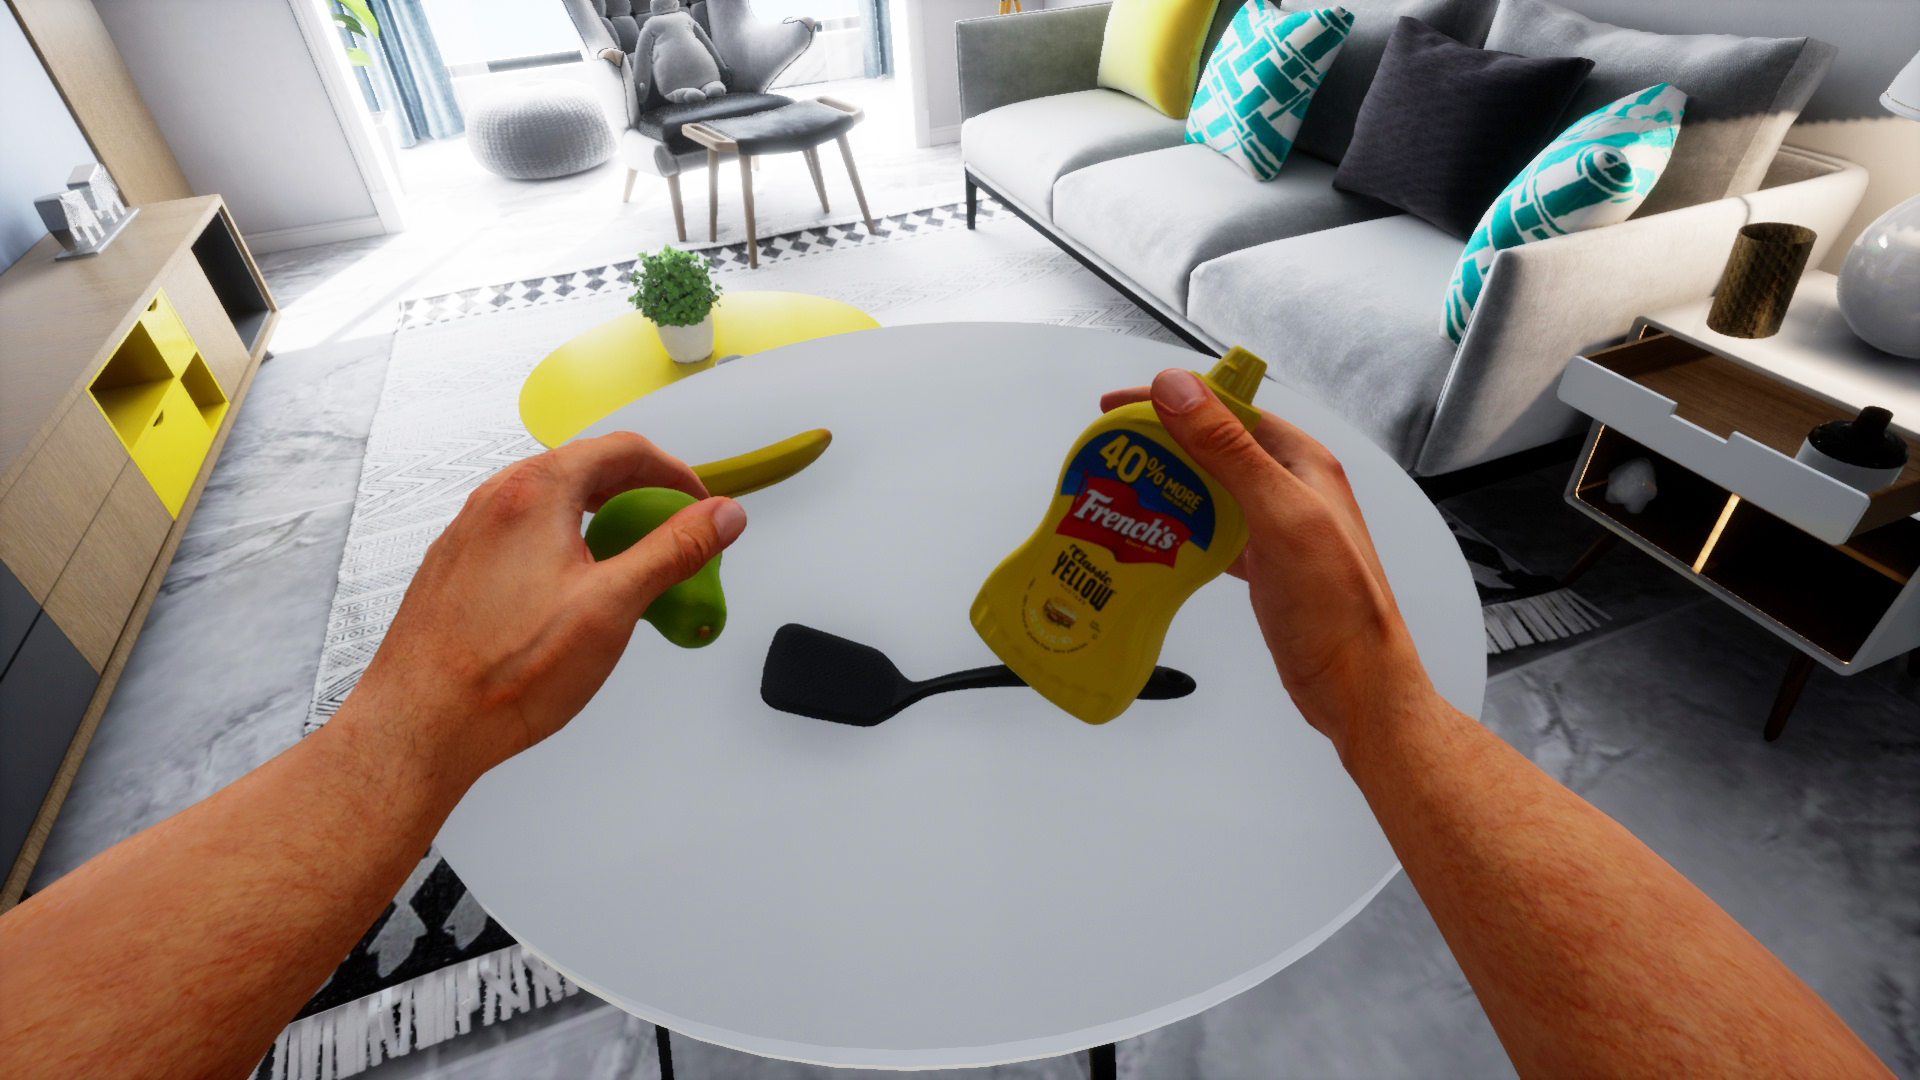
\includegraphics{figures/unrealgrasp/real_0.jpg}}
		\label{subfig:resampling_vector}}
	\subfloat[]{\resizebox{0.49\textwidth}{!}{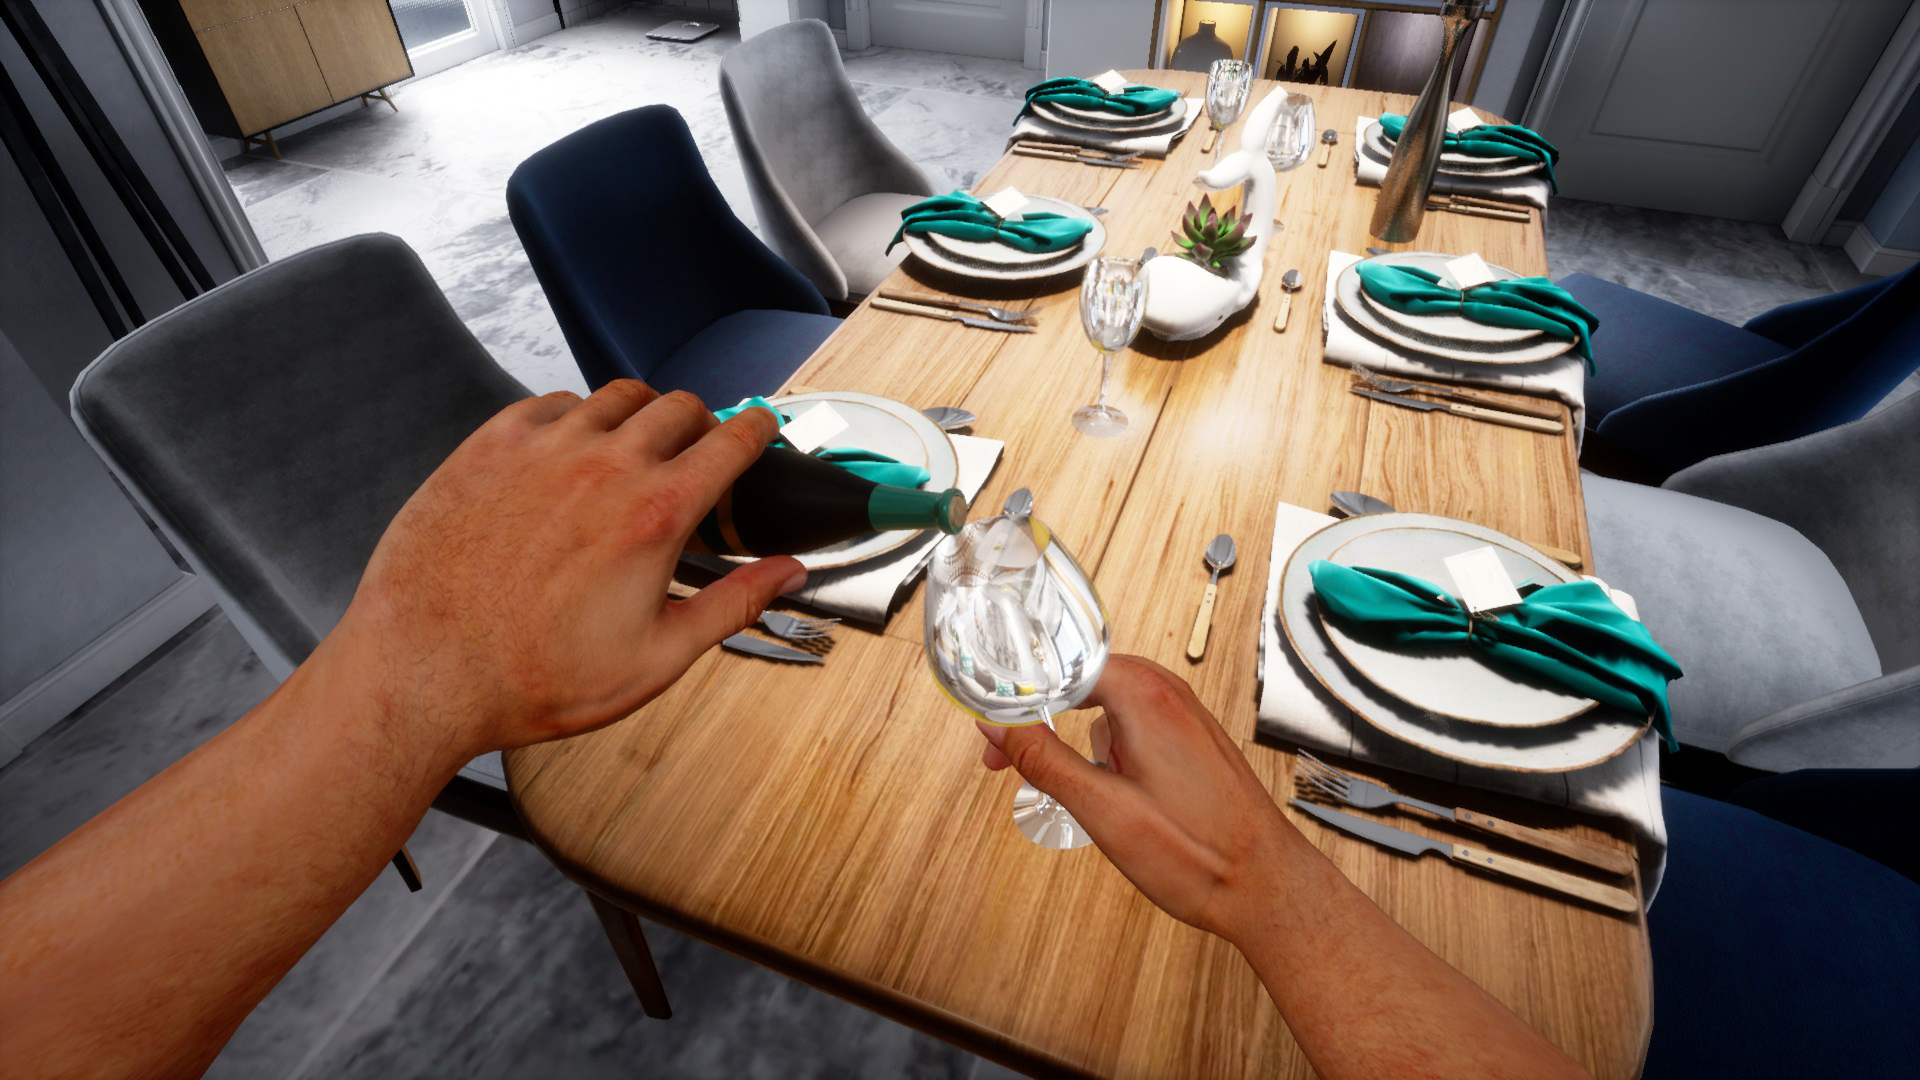
\includegraphics{figures/unrealgrasp/real_1.jpg}}
		\label{subfig:resampling_vector}}
	\\
	\subfloat[]{\resizebox{0.49\textwidth}{!}{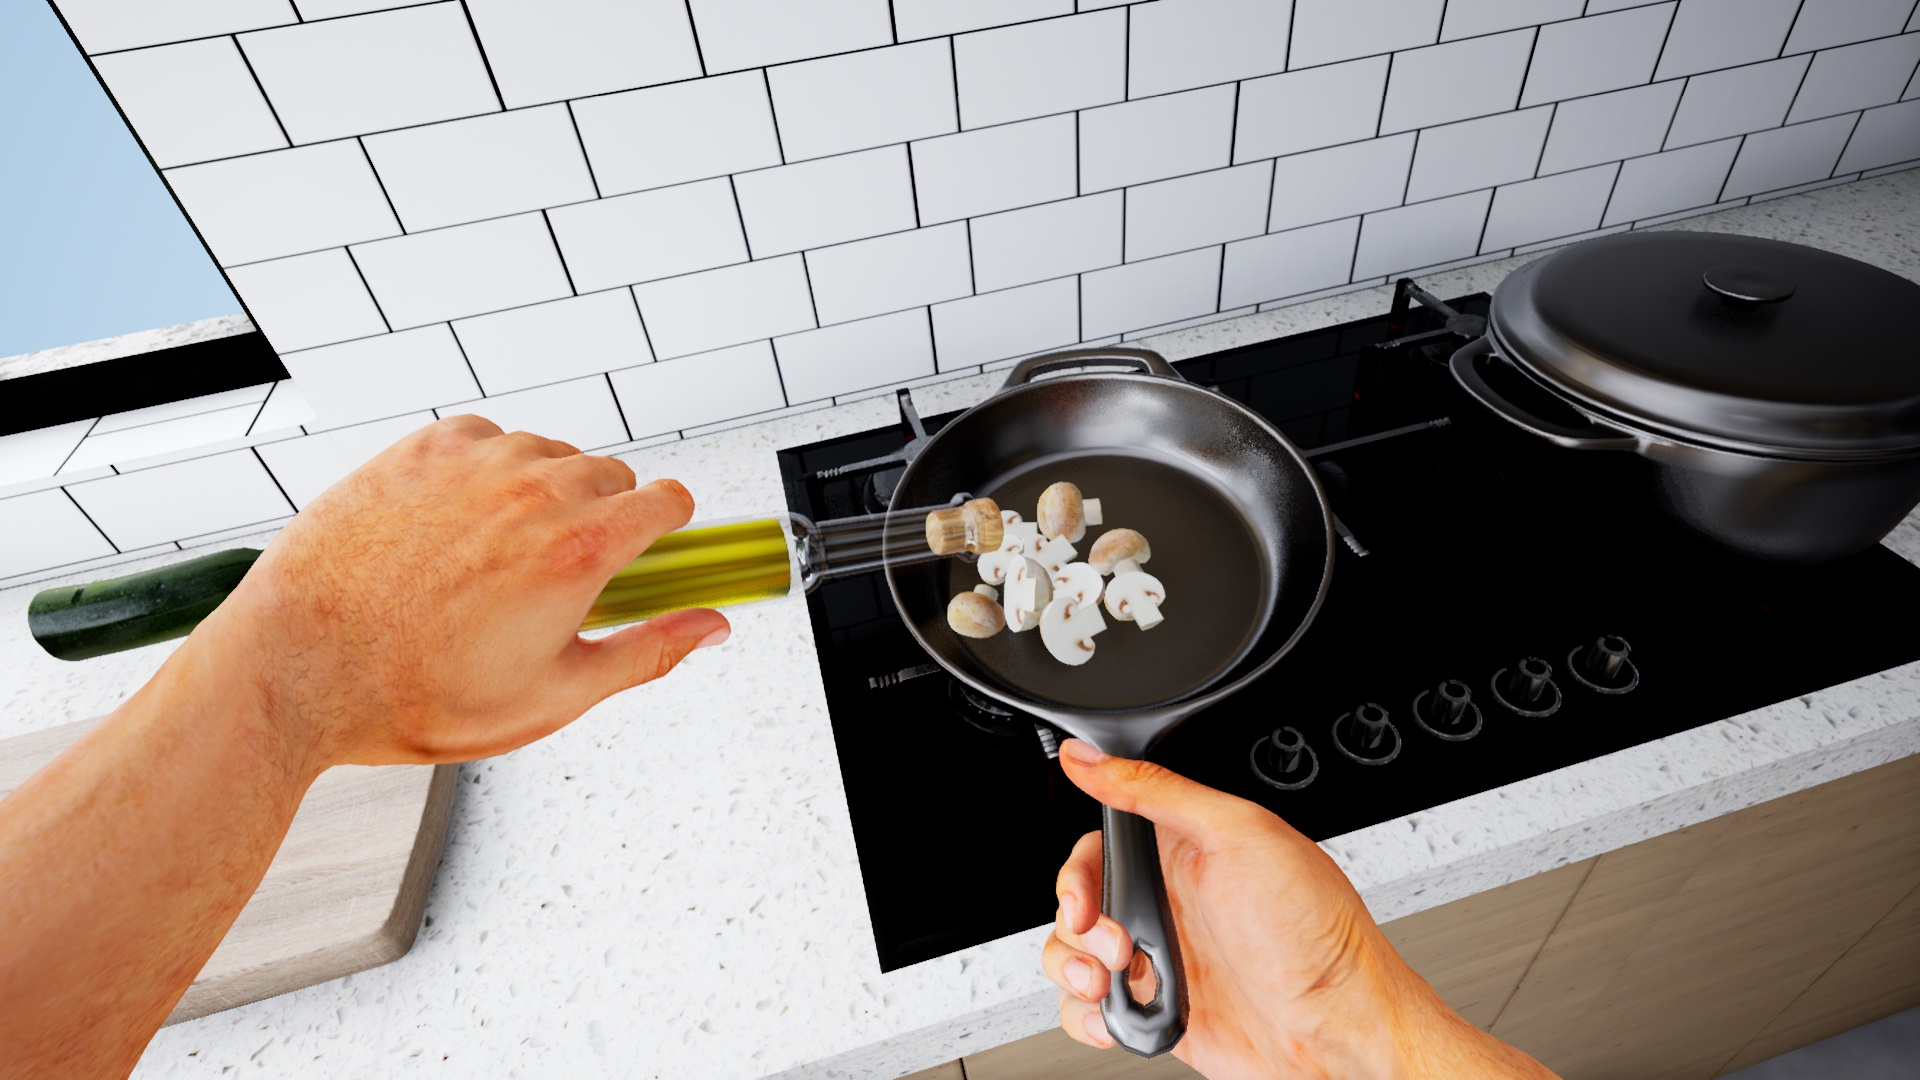
\includegraphics{figures/unrealgrasp/real_2.jpg}}
		\label{subfig:resampling_vector}}
	\subfloat[]{\resizebox{0.49\textwidth}{!}{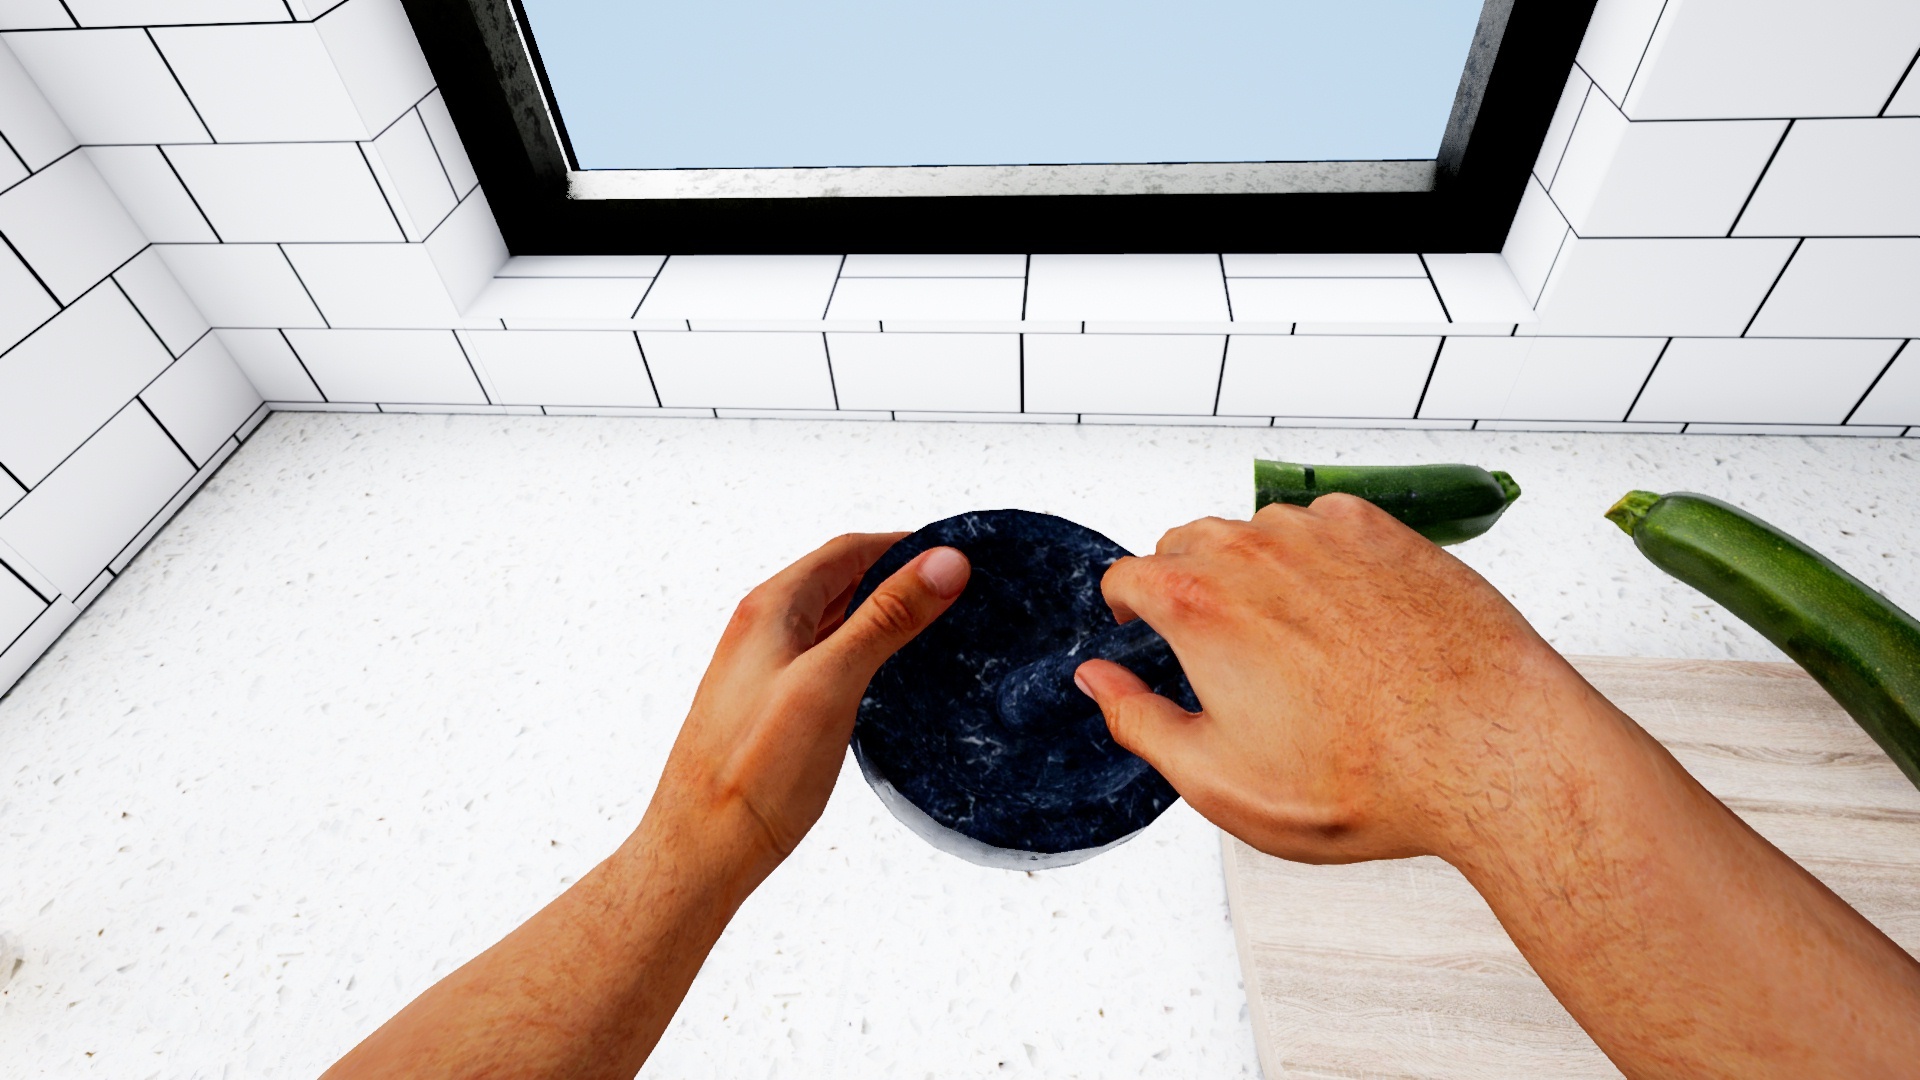
\includegraphics{figures/unrealgrasp/real_3.jpg}}
		\label{subfig:resampling_vector}}
	\caption{The user interacts with objects extracted from the YCB dataset in a photorealistic virtual environment.}
	\label{fig:interaction}
\end{figure}

Our grasping system was analyzed both qualitatively and quantitatively. On one side, for the qualitative analysis, grasping system was implemented in a photorealistic environment where the user is freely able to interact with real world objects extracted from the YCB dataset \cite{calli2015} (see Figure \ref{fig:interaction}). The qualitative evaluation is based on a questionnaire that will address the user interaction experience in terms of realism during object manipulation, system flexibility and usability, and general VR experience. On the other side, a quantitative grasping system analysis was carried out, contrasting the elapsed time a user needs in grasping an object and grasp quality based on a novel error metric which quantifies the overlapping between hand fingers and the grasped object. From the quantitative evaluation, we obtain the individual errors for the last two phalanges of each finger, the time user needed to grasp the object and also the contact points in both local and global system coordinates. The performance evaluation shows that the interaction is natural even if it is not mimicking the movement patterns of the physical world (i.e. user fingers do not close the same way as the virtual fingers). Implementation and demo videos are available at Github\footnote{\href{https://github.com/3dperceptionlab/unrealgrasp}{https://github.com/3dperceptionlab/unrealgrasp}}.

In summary, we make two main contributions:
\begin{itemize}
	\item We propose a novel, robust and flexible grasping system for real-time interactions in virtual reality environments, where hand is automatically fitted to the object shape from a 6D position determined by the user using a pair of handheld controllers;
	\item We define a novel metric and procedure to visually analyze grasping quality in VR interactions quantifying hand-object overlapping; 
\end{itemize}

The rest of the paper is structured as follows. First of all, Section \ref{sec:related_works} analyzes the latest works related to object interaction and manipulation in virtual environments. The core of this work is comprised in Section \ref{sec:graspingsystem} where our approach is described in detail. Then, the performance analysis, with the qualitative and our novel quantitative evaluations, is discussed in Section \ref{sec:experimentation}. Analysis results are reported in Section \ref{sec:results}. Then, several applications are discussed in Section \ref{sec:applications}. After that, limitations of our approach are covered in Section \ref{sec:limitationsfutureworks} alongside several feature works. Finally, some conclusions are drawn in the last Section \ref{sec:conclusion}.

\section{Related works}
\label{sec:related_works}
Grasping action is the most basic component of any interaction and it is composed of three major components \cite{aydin1999}. The first one is related to the process of approaching the arm and hand to the target object, considering the overall body movement. The second component focuses on the hand and body pre-shaping before the grasping action. Finally, the last component fits the hand to the object geometry by closing each of the fingers until contact is established.

Our work and most of the existing works related to the interaction in VR environments, are related to the third component of the grasping pipeline. Most of the existing real-time approaches are based purely on multiple predefined animations for each object the user will interact with, relying completely on the animation quality. Consequently, they are unable to deal with unknown objects without any associated predefined animation for each. This fact limits the user experience and its immersion in the VR environments by hindering their interaction capabilities.

This section contains the most recent works which are mostly aligned with our proposal where interaction is done by means of handheld controllers (e.g. Oculus VR and HTC Vive PRO controllers). In addition to these approaches, there are other interesting works considered as a valuable source of inspiration. For example, Verschoor et al. proposed a soft-hand model simulation defined as a unified energy minimization problem achieving impressive results with natural and intuitive real-time interactions \cite{Verschoor2018}. On the other hand, haptic simulation of grasping is another promising way to improve interaction in virtual environments, highlighting the work proposed by Garre et al. \cite{Garre2011}.

\subsection{Data-driven approaches}
Grasping data-driven based approaches have existed since a long time ago \cite{aydin1999}. These methods work alongside large databases containing predefined hand poses, each one associated to a concrete object geometry. The most suitable grasp pose is selected according to the defined grasp taxonomy or based on the user criteria. Most of the currently existing approaches for grasping are data-driven. The key of data-driven approaches is to effectively index large datasets in order to quickly match unknown object geometries with the most suitable hand pose from the database \cite{li2007} \cite{goldfeder2011}.

Li et al. \cite{li2007} constructed a database of hand poses for different object shapes and sizes. Despite having a good database, the process of hand pose selection was not straightforward since there can be multiple equally valid possibilities for the same object. To address this problem, Li et al. \cite{li2007} proposed a shape-matching algorithm which returns multiple potential grasp poses. The selection process is also limited by the hand high degree of freedom (DOF). In order to deal with dimensionality and redundancy many researchers have used techniques such as principal component analysis (PCA) \cite{braido2004}\cite{ciocarlie2007}. For the same purpose, Jorg et al. \cite{jorg2009} studied the correlations between hand DOFs aiming to simplify hand models reducing DOF number. 

In order to achieve realistic object interactions, other approaches also considered physical constraints \cite{pollard2005}\cite{kry2006}\cite{bai2014}. By using an initial grasp pose and a desired object trajectory, the algorithm proposed by Liu \cite{liu2009} can generate physically-based hand manipulation poses varying the contact points with the object, grasping forces and also joint configurations. Since hand and finger movement trajectories need to be both, kinematically and dynamically valid, Ye and Liu \cite{ye2012} reconstruct a realistic hand motion and grasping generating feasible contact point trajectories. 


\subsection{Virtual reality approaches}

This section is focused on the virtual reality approaches where interactions are performed using VR motion controllers, avoiding glove-based and bare-hand approaches. Implementation of the aforementioned techniques in virtual reality environments is a difficult task cause optimizations are needed to keep processes running in real-time. Most of the existing approaches for interaction in VR applications lack of realism. The existing trend is to create efficient solutions to enable real-time interactions leaving in the background interaction realism. 

Recent approaches are directly related to the entertainment industry, i.e. video games. An excellent example is \emph{Lone Echo}, a narrative adventure game which consists of manipulating tools and objects for solving puzzles. Hand animations are procedurally generated, enabling grasping of complex geometries regardless their grasp angle. This approach \cite{copenhaver2017} is based on a graph traversal heuristic which searches intersections between hand fingers and object surface mesh triangles. This is the A* heuristic, which finds the nearest palm intersections, and also filtering the invalid ones. After calculating angles to make contact with each intersection point, highest angle is selected and fingers are rotated accordingly.

Other available solutions focusing the interaction in VR are animation-based \cite{oculusDistanceGrab2017} \cite{oculusFirstExperience} \cite{vrtemplate2016}. In these approaches, user interaction with the virtual environment is limited to the objects that have a predefined grip animation. Resulting interaction is smooth and visually realistic, however it ends in a repetitive and unnatural behavior. In \cite{oculusDistanceGrab2017}, distance grab selection technique was implemented to enhance the user comfort when interacting in small play areas, while sitting or for grabbing objects on the floor. Grasping system is based on three trigger volumes attached to each hand: two small cylinders for short-range grasp, and a cone for long-range grabbing. Inspired on this approach, we adopted the usage of trigger volumes which attached to the finger phalanges we are able to control its movement and fit the hand to the object shape. 

In contrast with the available VR approaches, our system does not implement the distance grab technique (i.e. users can point to faraway objects, and have them leap into the hands when squeezing the grip button) as in \cite{oculusDistanceGrab2017}. Due to, applying our proposed performance evaluation would be not fair nor feasible. A rough comparison with similar approaches would be in terms of interaction speed, realism and naturalness. With our approach users will take longer to grasp objects as they need to previously place and orient the hand in accordance with the 6D object pose before grasping. However, these times will be increasingly shorter with practice in exchange for visually realistic results. Moreover and regarding the solution proposed in the \emph{Lone Echo} game, technical details are not sufficient to implement their proposal.


\section{Grasping system}
\label{sec:graspingsystem}

The user, embodied in the virtual environment, is able to control the position and orientation of his virtual hands using a pair of handheld controllers (for this work, the Oculus Touch and HTC Vive Pro controllers were used). These controllers are equipped with several buttons, triggers, thumbsticks and provide an accurate 6D one-to-one motion tracking. In order to grasp an object, the user would firstly position and orient the hands according to the 6D object pose and its geometry. When the hands are close enough to grasp the object, they can be closed by pressing a trigger button. In the case of Oculus Touch and HTC Vive Pro controllers, these are one-dimensional controls that report a floating point state, so the user can control the amount of closing or opening of their virtual hands (i.e. hand closing action can be stopped at any time). The system works independently of the button assigned for closing/opening action of the virtual hands, provided that it is an axis and returns floating point values depending on the amount of pressure being exerted. When closing the hand, finger movement is also conditioned by the object geometry. In other words, fingers stop moving when an overlap with the target object is detected. With this approach, hand is automatically fitted to the object shape. The user will unconsciously imitate a real human behavior when approximating his hands to grasp the virtual objects (e.g. the user will in first instance try to grab the kitchen spatula by its handle), so that the resulting interactions will be visually realistic and natural.

\subsection{Overview}
\label{subsec:overview}

Our grasping approach was designed to enable real-time interaction and manipulation in virtual reality environments by providing a simple, modular, flexible, robust, and visually realistic grasping system. Featuring an intuitive object manipulation, the interaction in VR environments results in a pleasant experience. Its main features are described as follows:

\begin{itemize}
	\item Simple and modular: system design is modular and easily customizable and extensible. All the components described in the next section can be easily modified and adapted to handle different scenarios.
	\item Flexible: our approach is flexible because it can be adapted to different hand meshes (e.g. human hand or robotic hand) without much effort. 
	\item Robust: it allows the manipulation of different objects regardless of their geometries. Most existing approaches are based on knowing or detecting the shape of the object beforehand in order to choose the best grasp from a database, or using other related techniques. Our approach enables real-time manipulation of unknown objects because hand is automatically fitted to their shapes.
	\item Visually realistic: resulting graspings are visually realistic because hand is automatically fitted to the object shape beginning from a position determined by the user using the VR handheld controllers, such as Oculus Touch or HTC Vive PRO. In other words, positioning and orienting the hand in order to grab the object is up to the user. Most of the users unconsciously would try to grasp the virtual objects such as they would be real, e.g. the user would tend to grab a hammer by its handle.
\end{itemize}

The essence of our grasping system is how the hand is automatically fitted to the object shape. The main idea behind, is to keep moving the fingers when closing the hand until a collision with the object to be grasped is detected. Through the use of trigger actors placed experimentally on the last two phalanges of each finger, we could detect when a specific finger is in contact with the manipulated object. 


\subsection{Grasp animation and trigger placement}

In order to choose the most appropriate hand closing animation we analyzed the grasp taxonomy proposed by Feix et al. \cite{feix2016grasp} in which we can find 33 different grasp types arranged according to power/precision requirements, opposition type (palm, pad or side opposition) and thumb position (abducted or adducted). On the basis of this taxonomy a common pattern has been identified in multiple power grips when manipulating objects of different geometries and sizes. This pattern is the cylindrical grasp, and it was suitable to imitate the different grips proposed in the taxonomy (e.g. power sphere, medium wrap, large diameter, etc.). This pattern is directly related to "power grasp" in which, according to Landsmeer \cite{Landsmeer1962}, the fingers and thumb wrap the object (i.e. there is a rigid relationship between the object and hand movement). In contrast, the "precision handling" is commonly used to manipulate (e.g. tip pinch) an object using the index, middle and thumb finger pads. In this case, and also for intermediate grips, several animations are needed, which implies selecting the proper animation according to the object being manipulated. However, to keep the grasping pipeline simple, we initially focused on power grasp using the cylindrical grip as a single hand closing animation.

Each grasp can be also classified according to the direction in which the hand is applying forces on the object to achieve a stable grasp. There are three basic grasping opposition types in which the direction of applied force varies:

\begin{figure}[!t]
	\centering
	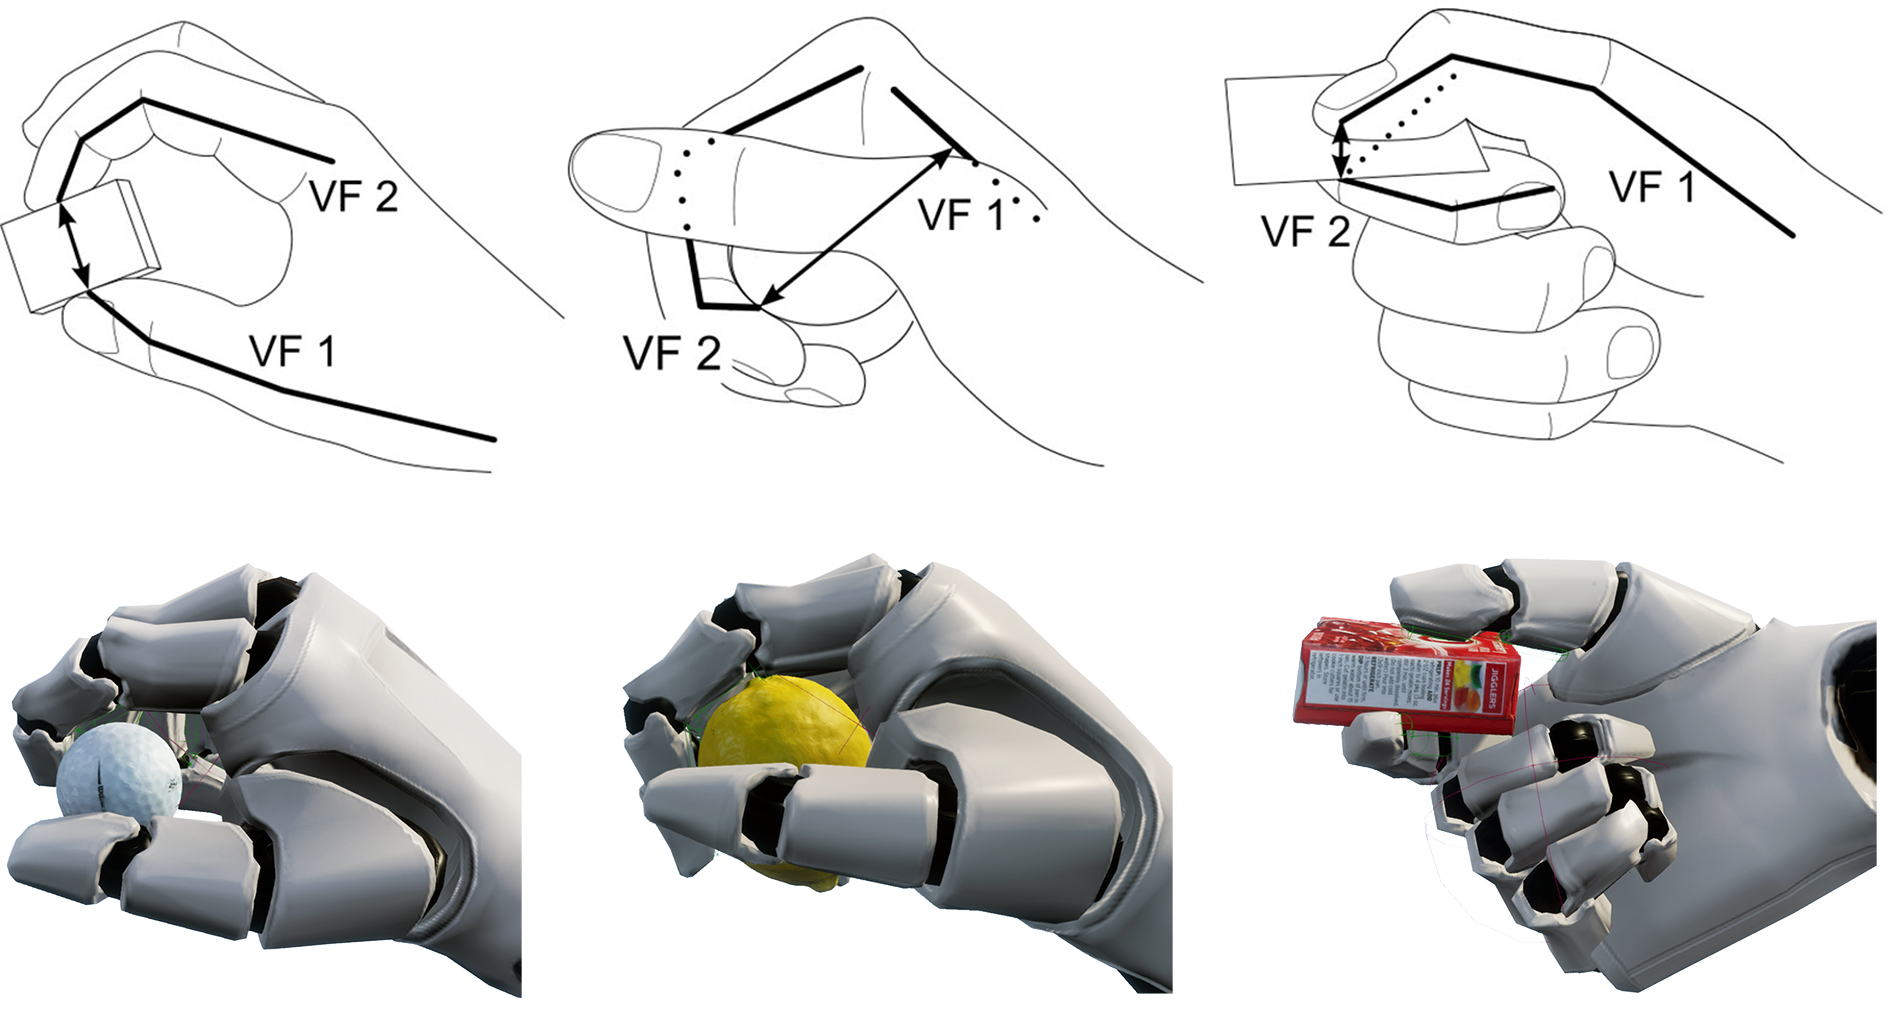
\includegraphics[width=0.95\linewidth]{figures/unrealgrasp/grasp_taxonomy.jpg}
	\caption{Represented from left to right the three different opposition types of the grasping hand: pad opposition, palm opposition, side opposition. The abbreviation VF refers to Virtual Finger. Figure adapted from \cite{feix2016grasp}.}
	\label{fig:grasp_taxonomy}
\end{figure}

\begin{itemize}
	\item Pad Opposition: force direction is usually parallel to hand palm. This opposition type is commonly used in precision grips which are performed using palmar surface and fingertips. This is represented in Figure \ref{fig:grasp_taxonomy} (bottom left) where a golf ball is attempted to be grasped using thumb and index fingertips. Regarding the grasp performed using our grasping system, it not represent an accurate "pinch" grasp. This is mainly because the closing hand animation was designed specifically for power grasp, performing worse in precision handling.
	\item Palm Opposition: commonly used in power grip, where forces on the object are mostly perpendicular to the palm and fingers wrap the object. As we can see in the Figure \ref{fig:grasp_taxonomy}, the lemon is accurately grasped between all the fingers and palmar surface, indicating that our approach was designed for power grip using palm opposition.
	\item Side Opposition: forces on the object are commonly applied transversally to the palm of the hand. With our virtual hand configuration and the capsule trigger placement, we can only detect overlapping at the fingertips. Consequently, our approach is not able to effectively perform side opposition grips. For a lateral grasp, we would have to change the size of the capsule triggers so that they stand out on the sides, or, place other triggers on the finger sides, thus increasing the complexity of our grasping system. In the Figure \ref{fig:grasp_taxonomy} (bottom right), the capsule trigger placed on the distal index phalanx is slightly in contact with the box, thus a lateral grip is possible. However, it is not straightforward to replicate this situation.	
\end{itemize}



\subsection{Trigger placement}

\begin{figure}[!t]
	\centering
	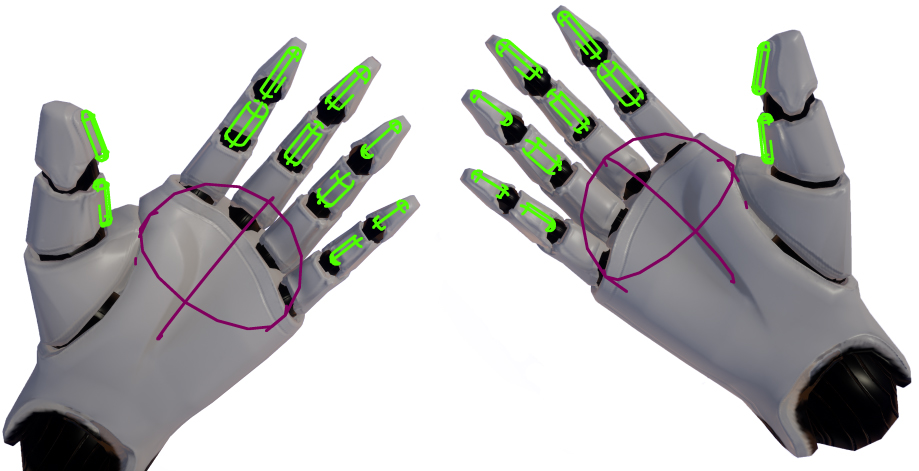
\includegraphics[width=.8\linewidth]{figures/unrealgrasp/mannequin_hands.jpg}
	\caption{Represented in green, the capsule triggers of the middle and distal phalanges. In purple, sphere trigger of the palm used to detect the nearest object to be grasped.}
	\label{fig:mannequinhands}
\end{figure}

A trigger actor is a component from Unreal Engine 4, and other engines such as Unity, used for casting an event in response to an interaction, e.g. when the trigger overlaps an object. Trigger placement on finger phalanges was done experimentally during the interaction with objects of varied geometry from the YCB dataset. This experimentation consisted mainly on determining the number of triggers to achieve a good behavior when interacting with different sized objects and varied shapes. Trigger overlapping is checked for each frame, thus using a large number of triggers would harm system performance. Due to, trigger number has been increased progressively during the experimentation. Firstly, interaction with small and different shaped objects (e.g. cubes, spheres, cones, etc.) was performed only using triggers on the distal phalanges. The results were convincing, however, when dealing with larger objects, they were slippery in the hand until the distal triggers made contact with the object. This slippery behavior was due to the fact that the middle phalanges collided with the object before the distal ones, so the solution was to add triggers to the middle phalanges to stop their movement when overlapping with the object. Finally, a sphere trigger has been added to the hand palm in order to use the palmar surface when grasping, such as in pad and palm oppositions. This has improved interaction with small objects. The final hand configuration is represented in Figure \ref{fig:mannequinhands}.

\subsection{Grasping pipeline components}


\definecolor{lightgreen}{RGB}{166,196,138}
\definecolor{lightblue}{RGB}{143,184,237}

\tikzstyle{block} = [rectangle, draw, fill=lightgreen, 
text width=5em, text centered, rounded corners, minimum height=3em]
\tikzstyle{cloud} = [draw, ellipse, text centered, fill=lightblue, text width=4em,
minimum height=2em]
\tikzstyle{line} = [draw, -latex']

\begin{figure}[!t]
	\centering
	\resizebox{0.7\textwidth}{!}{
		\begin{tikzpicture}[node distance = 3.0cm, auto]
		% Place nodes
		\node [block] (init) {Object selection};
		\node [block, right of= init] (manager) {Interaction manager};
		\node [block, right of= manager] (movement) {Finger movement};
		\node [block, right of= movement] (logic) {Grasping logic};
		
		% Draw edges
		\path [line] (init) -- (manager);
		\path [line] (manager) -- (movement);
		\path [line] (movement) -- (logic);
		\end{tikzpicture}}$  $
	\caption{Pipeline with the components of our grasping system.}
	\label{fig:pipeline}
\end{figure}

Our grasping system is composed of the components shown in the Figure \ref{fig:pipeline}. They are defined as follows:
\begin{itemize}
	\item Object selection: selects the nearest object to the hand palm. Graspable area is determined by a sphere trigger placed on the hand palm (red colored in Figure \ref{fig:mannequinhands}). The sphere trigger returns the world location of all the overlapped actors. As a result, the nearest actor can be determined by computing the distance from each overlapped actor to the center of the sphere trigger. Smallest distance will determine the nearest object.
	\item Interaction manager: manages the capsule triggers attached to the finger phalanges as represented in Figure \ref{fig:mannequinhands}. If a capsule trigger reports an overlap event, the movement of its corresponding phalanx is blocked until hand is reopened or the overlapping with the manipulated object is over. The phalanx state (represented as a boolean value, blocked or released) will be used as input to the grasping logic component and determines when the phalanx is movable. A phalanx is defined as blocked when its attached capsule trigger is overlapping with the object being manipulated. In other words, this indicates which phalanges are in contact with the object.
	\item Finger movement: this component controls the movement of the fingers during the hand closing and opening animations. It ensures a smooth animation avoiding unexpected and unrealistic behavior during finger movement caused neither by a performance drop or other interaction issues. Basically, it monitors the variation in the movement of each phalanx. When detecting an unexpected variation, i.e. the difference in the phalanx movement during a frame change is bigger than a threshold value, missing intermediate values will be interpolated so as to keep finger movement smooth. 
	\item Grasping logic: this component decides when to grab or release an object. The decision is made based on the phalanx state provided by the interaction manager component, e.g. at least a phalanx of the thumb and index fingers need to be in contact with the manipulated object in order to perform a top pinch grasp. 
	
	The object is grasped or released according to the following function which operates using boolean values as inputs indicating when finger phalanges are in contact or not with the object:
	
	\begin{equation} \label{eq:3}
	f(th_{ph}, in_{ph}, mi_{ph}, palm)= 
	\begin{cases}
	true, & \text{if } (th_{ph} \lor palm) \\
	& \land (in_{ph} \lor mi_{ph})\\
	false,              & \text{otherwise}
	\end{cases}
	\end{equation}, where $th_{ph}$, $in_{ph}$, and $mi_{ph}$ are defined as
	
	\begin{equation} \label{eq:4}
	\begin{array}{l}
	th_{ph} = thumb_{mid} \lor thumb_{dist} \\
	in_{ph} = index_{mid} \lor index_{dist} \\
	mi_{ph} = middle_{mid} \lor middle_{dist} \\
	\end{array}
	\end{equation}
	
	Equation \ref{eq:3} determines when an object is grasped or released based on the inputs determined in Equation \ref{eq:4} and palm trigger state. $th_{ph}$, $in_{ph}$, and $mi_{ph}$, represent the OR logic operator between their middle and distal phalanges values, respectively. In other words, this indicates it is enough to detect contact only with one of the two phalanges to state that the finger is interacting with the object (e.g. thumb finger is interacting with an object when a contact with the distal or middle phalanx is detected). According to human hand morphology, $mid$ and $dist$ subscripts refer to the middle and distal phalanx (e.g. $thumb_{dist}$ references the distal phalanx of thumb finger and at the implementation level it is a boolean value).
\end{itemize}


\subsection{Implementation details}

Grasping system has been originally implemented in Unreal Engine 4 (UE4), however, it can be easily implemented in other engines such as Unity, which would also provide us with the necessary components for replicating the system (e.g. overlapping triggers). The implementation consists of UE4 blueprints and has been correctly structured in the components depicted in Figure \ref{fig:pipeline} and described in the previous section. Implementation is available at Github (\url{https://github.com/3dperceptionlab/unrealgrasp}) using different UE4 versions.

\section{Performance analysis}
\label{sec:experimentation}

In order to validate our proposal, a complete performance analysis has been carried out. This analysis covers from a qualitative evaluation, which is prevalent in the assessment of VR systems, to a novel quantitative evaluation. Evaluation methods are briefly described as follows:
\begin{itemize}
	\item Qualitative evaluation: based on the user experience interacting with real objects from the YCB dataset in a photorealistic indoor scenario. Its purpose is to assess interaction realism, immersion, hand movement naturalness and other qualitative aspects described in Table \ref{table:questionnaire} from the Subsection \ref{subsec:qualitative}, which addresses qualitative evaluation in detail.
	\item Quantitative evaluation: based on the grasping quality in terms of realism (i.e. how much it is visually plausible). We consider a visually plausible grasp when hand palm or fingers are level with the object surface, as in a real life grasping. However, when dealing with complex meshes, the collision detection precision can be significantly influenced. In this case, fingers could penetrate the object surface, or remain above its surface when a collision was detected earlier than expected. This would result in an unnatural and unrealistic grasp. To visually quantify grasping quality, we propose a novel error metric based on computing the distance from each capsule trigger to the nearest contact point on the object surface. Quantitative evaluation and the proposed error metric are addressed in detail in Subsection \ref{subsec:quantitative}.
	
\end{itemize}


\subsection{Participants}

For the performance analysis, we recruited ten participants (8M/2F) from the local campus. Four of them have previous experience with VR applications (they have already used Oculus VR and HTC Vive headsets for gaming and/or developing purposes), as well as some of them may have previous experience using our system. The rest are inexperienced users, using a VR headset for the first time. Participants will take part on both qualitative and quantitative evaluation. The performance analysis procedure will be described in the following subsection, indicating the concrete tasks to be performed by each participant.

\subsection{Dataset}

To benchmark our grasping system we used a set of objects that are frequently used in daily life, such as, food items (cracker box, cans, box of sugar, fruits, etc.), tool items (power drill, hammer, screwdrivers, etc.), kitchen items (eating utensils) and also spherical shaped objects (tennis ball, racquetball, golf ball, etc.). Yale-CMU-Berkeley (YCB) Object and Model set \cite{calli2015} provides us these real-life 3D textured models scanned with outstanding accuracy and detail. Available objects have a wide variety of shapes, textures and sizes as we can see in Figure \ref{fig:ycbgrasps}. The advantage of using real life objects is that the user already has a previous experience manipulating similar objects so he will try to grab and interact with the objects in the same way.

\begin{figure}[!t]
	\centering
	\subfloat[Master Chef can]{\resizebox{0.24\textwidth}{!}{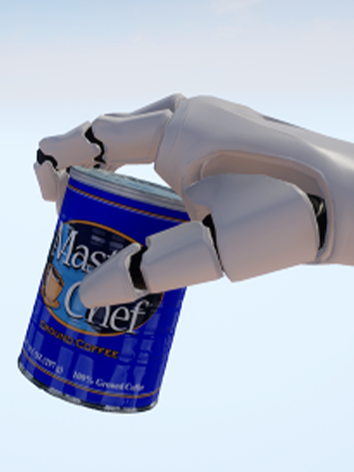
\includegraphics{figures/unrealgrasp/0.png}}
		\label{fig:masterchefcan}}
	\subfloat[Cracker box]{\resizebox{0.24\textwidth}{!}{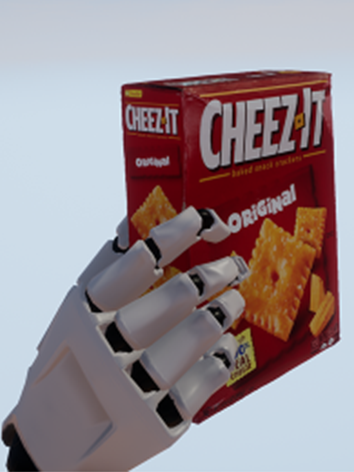
\includegraphics{figures/unrealgrasp/1.png}}
		\label{fig:crackerbox}}
	\subfloat[Sugar box]{\resizebox{0.24\textwidth}{!}{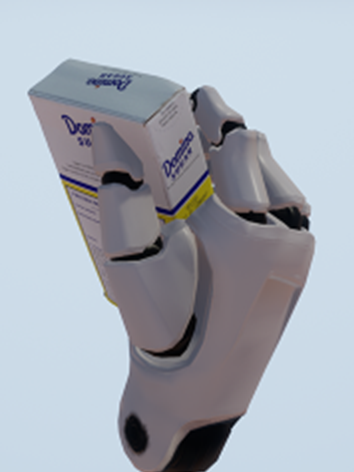
\includegraphics{figures/unrealgrasp/2.png}}
		\label{fig:sugarbox}}
	\subfloat[Tomato soup can]{\resizebox{0.24\textwidth}{!}{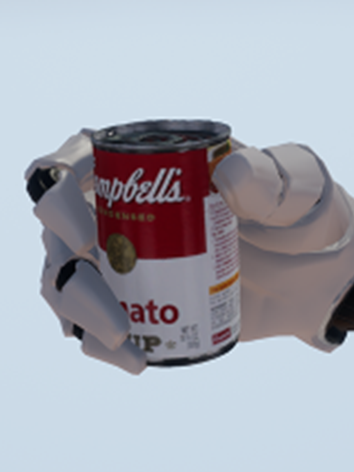
\includegraphics{figures/unrealgrasp/3.png}}
		\label{fig:tomatosoupcan}}
	\\
	\subfloat[Moustard bottle]{\resizebox{0.24\textwidth}{!}{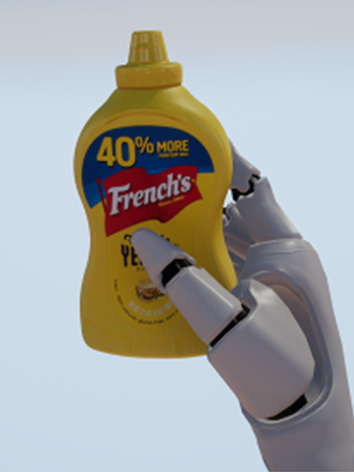
\includegraphics{figures/unrealgrasp/4.png}}
		\label{fig:mustardbottle}}
	\subfloat[Tuna fish can]{\resizebox{0.24\textwidth}{!}{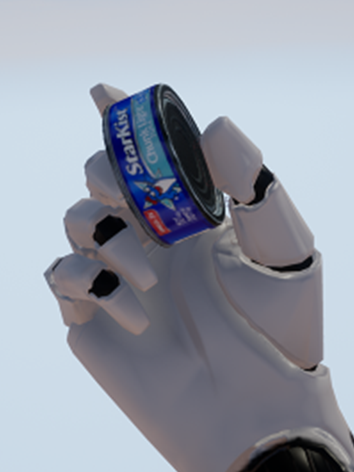
\includegraphics{figures/unrealgrasp/5.png}}
		\label{fig:tunafishcan}}
	\subfloat[Gelatin box]{\resizebox{0.24\textwidth}{!}{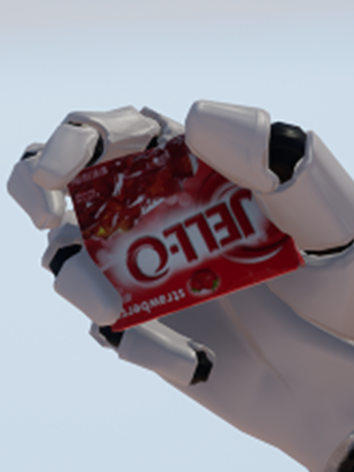
\includegraphics{figures/unrealgrasp/7.png}}
		\label{fig:gelatinbox}}
	\subfloat[Potted meat can]{\resizebox{0.24\textwidth}{!}{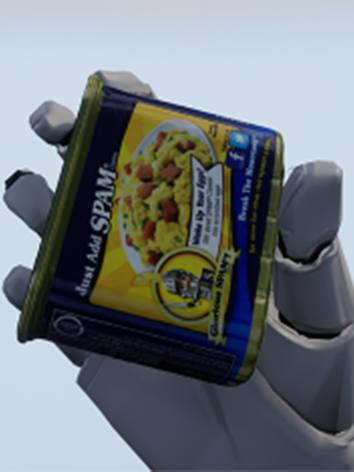
\includegraphics{figures/unrealgrasp/8.png}}
		\label{fig:pottedmeatcan}}
	\\
	\subfloat[Banana]{\resizebox{0.24\textwidth}{!}{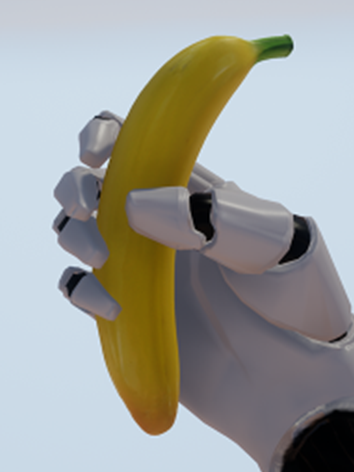
\includegraphics{figures/unrealgrasp/9.png}}
		\label{fig:banana}}
	\subfloat[Strawberry]{\resizebox{0.24\textwidth}{!}{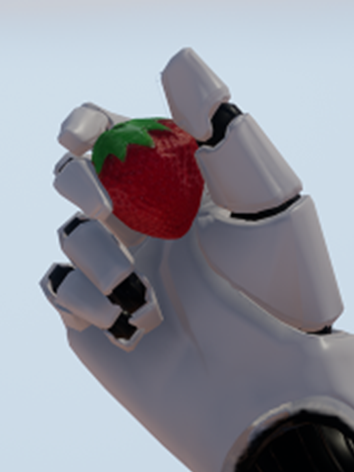
\includegraphics{figures/unrealgrasp/10.png}}
		\label{fig:strawberry}}
	\subfloat[Apple]{\resizebox{0.24\textwidth}{!}{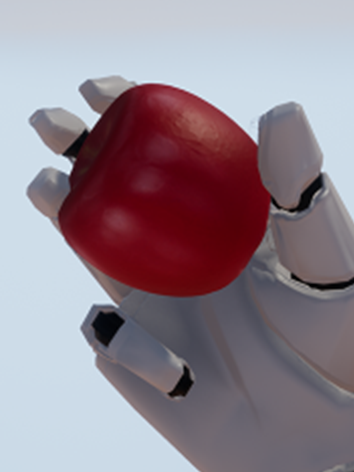
\includegraphics{figures/unrealgrasp/11.png}}
		\label{fig:apple}}
	\subfloat[Lemon]{\resizebox{0.24\textwidth}{!}{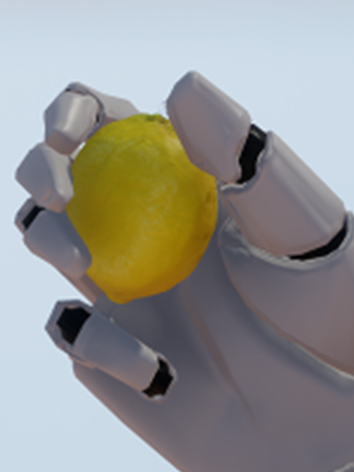
\includegraphics{figures/unrealgrasp/12.png}}
		\label{fig:lemon}}
	\\
	\subfloat[Peach]{\resizebox{0.24\textwidth}{!}{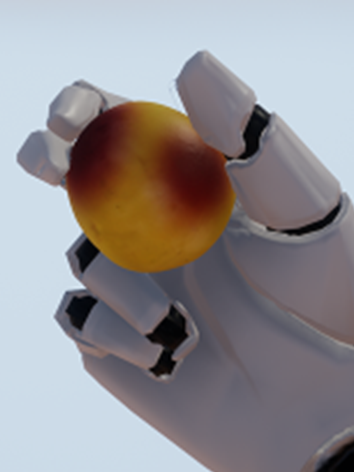
\includegraphics{figures/unrealgrasp/13.png}}
		\label{fig:peach}}
	\subfloat[Pear]{\resizebox{0.24\textwidth}{!}{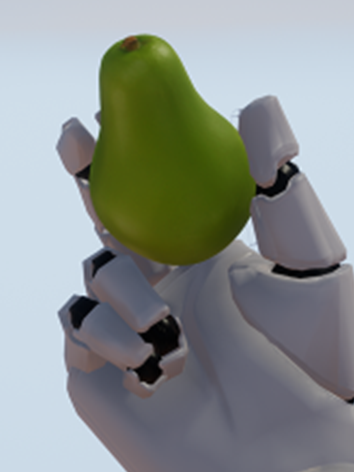
\includegraphics{figures/unrealgrasp/14.png}}
		\label{fig:pear}}
	\subfloat[Orange]{\resizebox{0.24\textwidth}{!}{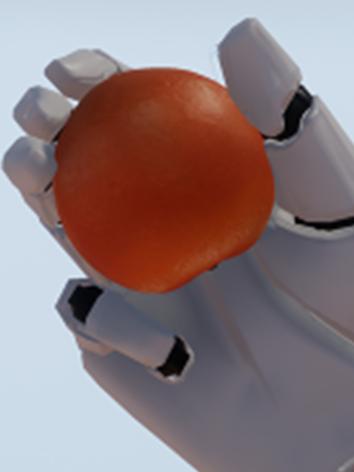
\includegraphics{figures/unrealgrasp/15.png}}
		\label{fig:orange}}
	\subfloat[Plum]{\resizebox{0.24\textwidth}{!}{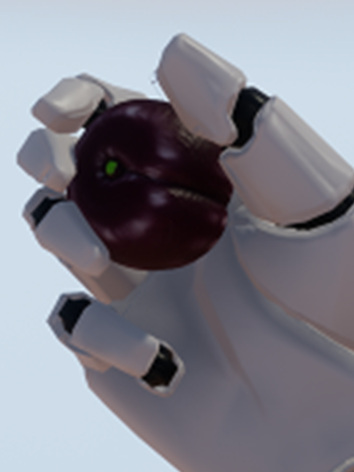
\includegraphics{figures/unrealgrasp/16.png}}
		\label{fig:plum}}
	\caption{Grasping performed on objects from the YCB dataset.}\label{fig:ycbgrasps}
\end{figure}

\begin{figure}[!t]
	\ContinuedFloat
	\centering
	\subfloat[Bleach cleaner]{\resizebox{0.24\textwidth}{!}{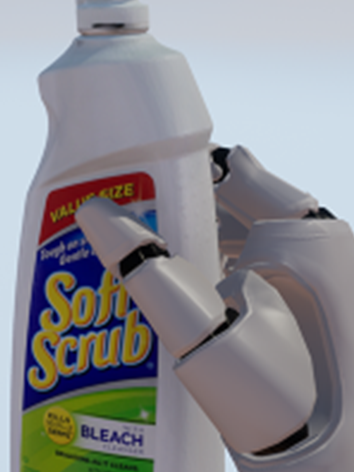
\includegraphics{figures/unrealgrasp/17.png}}
		\label{fig:bleachcleaner}}
	\subfloat[Fork]{\resizebox{0.24\textwidth}{!}{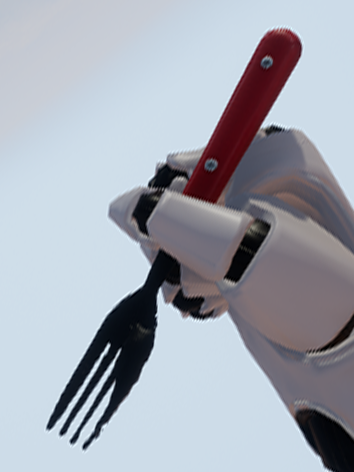
\includegraphics{figures/unrealgrasp/18.png}}
		\label{fig:fork}}
	\subfloat[Spoon]{\resizebox{0.24\textwidth}{!}{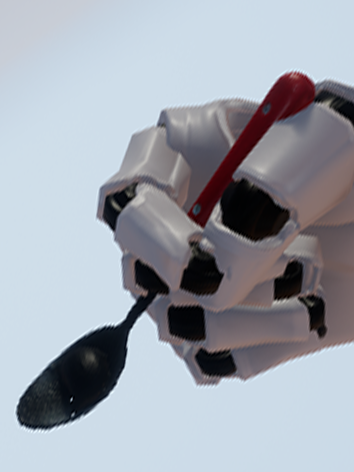
\includegraphics{figures/unrealgrasp/19.png}}
		\label{fig:spoon}}
	\subfloat[Knife]{\resizebox{0.24\textwidth}{!}{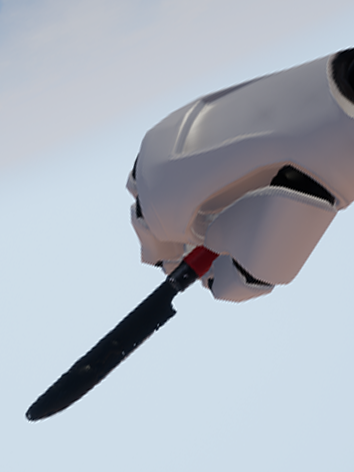
\includegraphics{figures/unrealgrasp/20.png}}
		\label{fig:knife}}
	\\
	\subfloat[Spatula]{\resizebox{0.24\textwidth}{!}{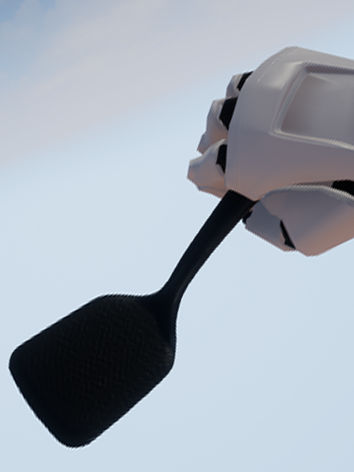
\includegraphics{figures/unrealgrasp/21.png}}
		\label{fig:spatula}}
	\subfloat[Power drill]{\resizebox{0.24\textwidth}{!}{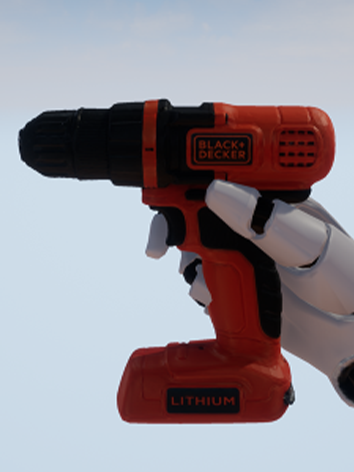
\includegraphics{figures/unrealgrasp/22.png}}
		\label{fig:powerdrill}}
	\subfloat[Scissors]{\resizebox{0.24\textwidth}{!}{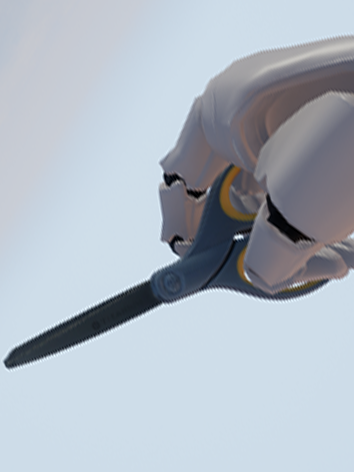
\includegraphics{figures/unrealgrasp/23.png}}
		\label{fig:scissors}}
	\subfloat[Large marker]{\resizebox{0.24\textwidth}{!}{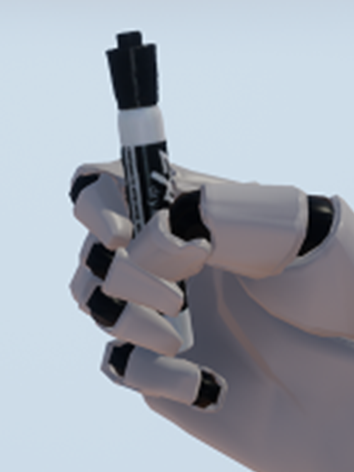
\includegraphics{figures/unrealgrasp/24.png}}
		\label{fig:largemarker}}
	\\
	\subfloat[Adjustable wrench]{\resizebox{0.24\textwidth}{!}{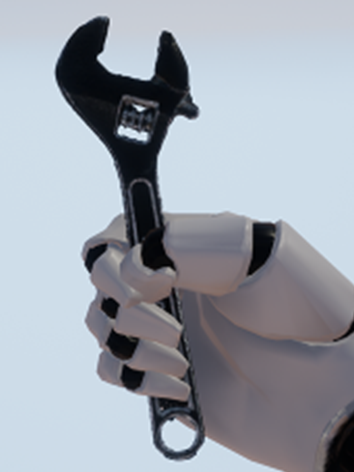
\includegraphics{figures/unrealgrasp/25.png}}
		\label{fig:adjustablewrench}}
	\subfloat[Flat screwdriver]{\resizebox{0.24\textwidth}{!}{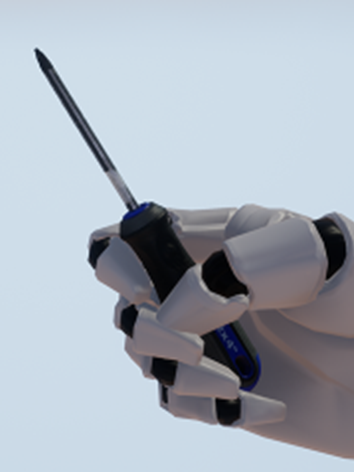
\includegraphics{figures/unrealgrasp/26.png}}
		\label{fig:flatscrewdriver}}
	\subfloat[Hammer]{\resizebox{0.24\textwidth}{!}{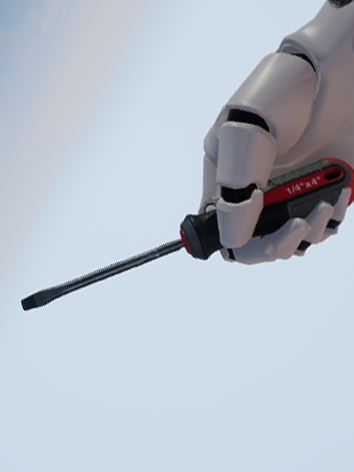
\includegraphics{figures/unrealgrasp/27.png}}
		\label{fig:hammer}}
	\subfloat[Baseball]{\resizebox{0.24\textwidth}{!}{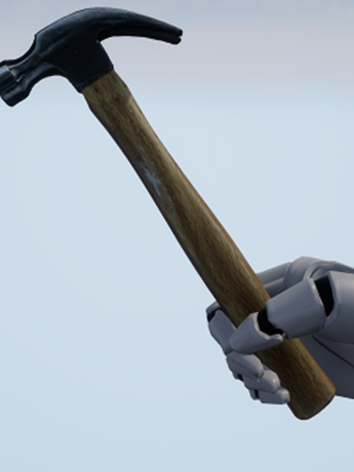
\includegraphics{figures/unrealgrasp/28.png}}
		\label{fig:baseball}}
	\\
	\subfloat[Tennis ball]{\resizebox{0.24\textwidth}{!}{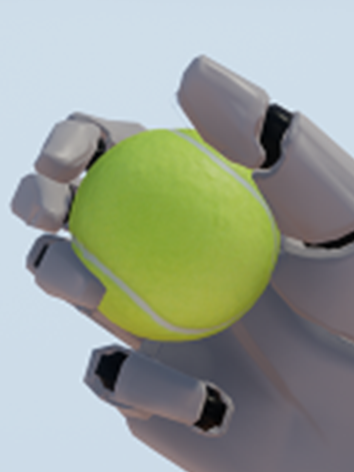
\includegraphics{figures/unrealgrasp/30.png}}
		\label{fig:tennisball}}
	\subfloat[Toy plane]{\resizebox{0.24\textwidth}{!}{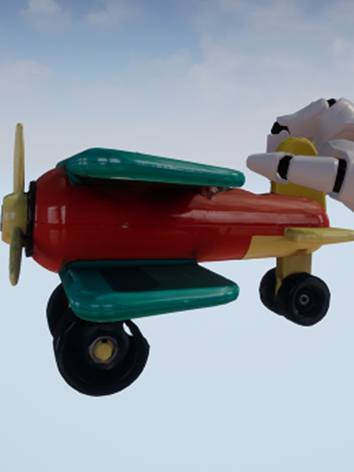
\includegraphics{figures/unrealgrasp/34.png}}
		\label{fig:toyplane}}
	\subfloat[Toy brick]{\resizebox{0.24\textwidth}{!}{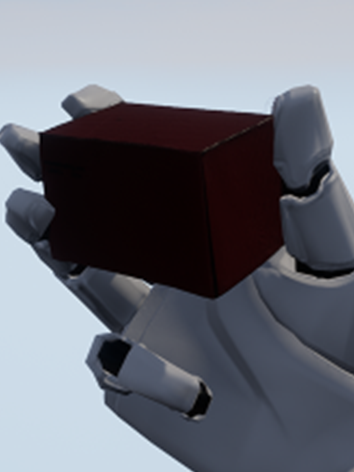
\includegraphics{figures/unrealgrasp/33.png}}
		\label{fig:toybrick}}
	\subfloat[Golf ball]{\resizebox{0.24\textwidth}{!}{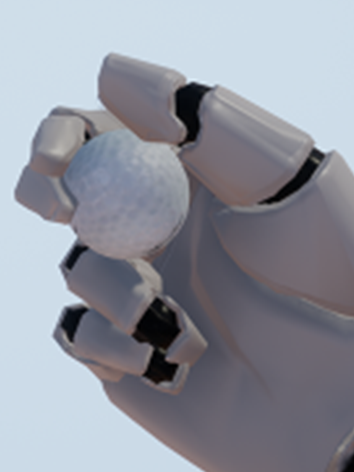
\includegraphics{figures/unrealgrasp/32.png}}
		\label{fig:golfball}}
	\caption{Grasping performed on objects from the YCB dataset.}\label{fig:ycbgrasps}
\end{figure}

\subsection{Qualitative evaluation}
\label{subsec:qualitative}

Most of VR experiments include qualitative and quantitative studies to measure its realism and immersion. Arguably, questionnaires are the default method to qualitatively assess any experience and the vast majority of works include them in one way or another \cite{Christopoulos2018} \cite{Koutsabasis2018} \cite{Vosinakis2018}. However, one of the main problems with them is the absence of a standardized set of questions for different experiences that allows for fair and easy comparisons. The different nature of the VR systems and experiences makes it challenging to find a set of evaluation questions that fits them all. Following the efforts of \cite{Gonzalez-Franco2018} towards a standardized embodiment questionnaire, we analyzed several works in the literature \cite{Poeschl2013} \cite{Brackney2017} that included questionnaires to assess VR experiences to devise a standard one for virtual grasping systems. Inspired by such works, we have identified three main types of questions or aspects:
\begin{itemize}
	\item Motor Control: this aspect considers the movement of the virtual hands as a whole and its responsiveness to the virtual reality controllers. Hands should move naturally and their movements must be caused exactly by the controllers without unwanted movements and without limiting or restricting real movements to adapt to the virtual ones.
	\item Finger Movement: this aspect takes the specific finger movement into account. Such movements must be natural and plausible. Moreover, they must react properly to the user's intent.
	\item Interaction Realism: this aspect is related to the interaction of the hand and fingers with objects. 
\end{itemize}

The questionnaire, shown in Table \ref{table:questionnaire}, is composed of fourteen questions related to the previously described aspects.
\begin{table}[!t]
	\resizebox{\linewidth}{!}{
		\begin{tabular}{cl}
			\hline
			\textbf{ID} & \textbf{Question}\\
			\hline
			\multicolumn{2}{c}{\emph{Aspect 1: Motor Control}}\\
			Q1 & I felt like I could control the virtual hands as if it were my own hands\\
			Q2 & The movements of the virtual hands were caused by my movements\\
			Q3 & I felt as if the movements of the virtual hands were influencing my own movements\\
			Q4 & I felt as if the virtual hands were moving by themselves\\
			\hline
			\multicolumn{2}{c}{\emph{Aspect 2: Finger Movement Realism}}\\
			\hline
			Q5 & It seemed that finger movements were smooth and plausible\\
			Q6 & I felt fingers open and close in a natural way\\
			Q7 & Fingers react adequately to my intentions\\
			\hline
			\multicolumn{2}{c}{\emph{Aspect 3: Interaction Realism}}\\
			\hline
			Q8 & I felt like I could grab objects wherever I wanted to\\
			Q9 & It seemed as if the virtual fingers were mine when grabbing an object\\
			Q10 & I felt that grabbing objects was clumsy and hard to achieve\\
			Q11 & It seemed as if finger movement were guided and unnatural\\
			Q12 & I felt that grasps were visually correct and natural\\
			Q13 & I felt that grasps were physically correct and natural\\
			Q14 & It seemed that fingers were adapting properly to the different geometries\\
			\hline
	\end{tabular}}
	\caption{User evaluation questionnaire.}
	\label{table:questionnaire}
\end{table}
Following \cite{Gonzalez-Franco2018}, the users of the study will be presented with such questions right after the end of the experience in a randomized order to limit context effects. In addition, questions must be answered following the 7-point Likert-scale: (+3) strongly agree, (+2) agree, (+1) somewhat agree, (0) neutral, (-1) somewhat disagree, (-2) disagree, and (-3) strongly disagree. Results will be presented as a single embodiment score using the following equations:
\begin{equation}\label{eq:6}
\begin{split}
\text{Motor Control} &= ((Q1 + Q2) - (Q3 + Q4)) / 4 \\
\text{Finger Movement Realism} &= (Q5 + Q6 + Q7) / 3 \\
\text{Interaction Realism} &= ((Q8 + Q9) - (Q10 + Q11) \\ 
& + Q12 + Q13 + Q14) / 7  
\end{split}
\end{equation}, using the results of each individual aspect, we obtain the total embodiment score as follows:
\begin{equation} \label{eq:5}
\begin{split}
\text{Score} &= (\text{Motor Control} + \text{Finger Movement Realism} \\
& + \text{Interaction Realism} * 2) / 4
\end{split}
\end{equation}

As far as the motor control aspect is concerned, it depends not only on our proposal, but also on the VR headset performance, for example, regarding headset and handheld controllers mapping and tracking. On the other hand, when referring to the finger movement realism aspect, this strongly relies on the quality and naturalness of the hand animation. Even so, interaction realism is the main objective of this work, and referring to the qualitative evaluation, it predominates in terms of the number of points to be evaluated.  So that, in the Equation \ref{eq:5} we emphasize this aspect by weighting it higher.

\subsection{Quantitative evaluation}
\label{subsec:quantitative}

With the quantitative evaluation, we aim to evaluate grasping quality in terms of how much it is visually plausible or realistic. In other words, we pursue to visually quantify our grasping performance, analyzing each finger position and how it fits the object mesh. When a collision is detected by a capsule trigger, we proceed with the calculation of the nearest distance between the finger phalanx surface (delimited by the capsule trigger) and the object mesh (see Equation \ref{eq:1}).

In Figure \ref{fig:distanceCalculus} the red capsules are representing 3D sphere tracing volumes which provide information of the nearest collision from the trace starting point to the first contact point on the object surface which intersects the sphere volume. For each finger phalanx with an attached capsule trigger represented in green, we throw a sphere trace obtaining the nearest contact points on the object surface represented as lime colored dots (impact point, Ip). In this representation, the total error for the index finger would be the average of the sum of the distances in millimeters between the surface of each phalanx and the nearest contact point on the object surface (see Equation \ref{eq:2}).
\begin{figure}[!t]
	\centering
	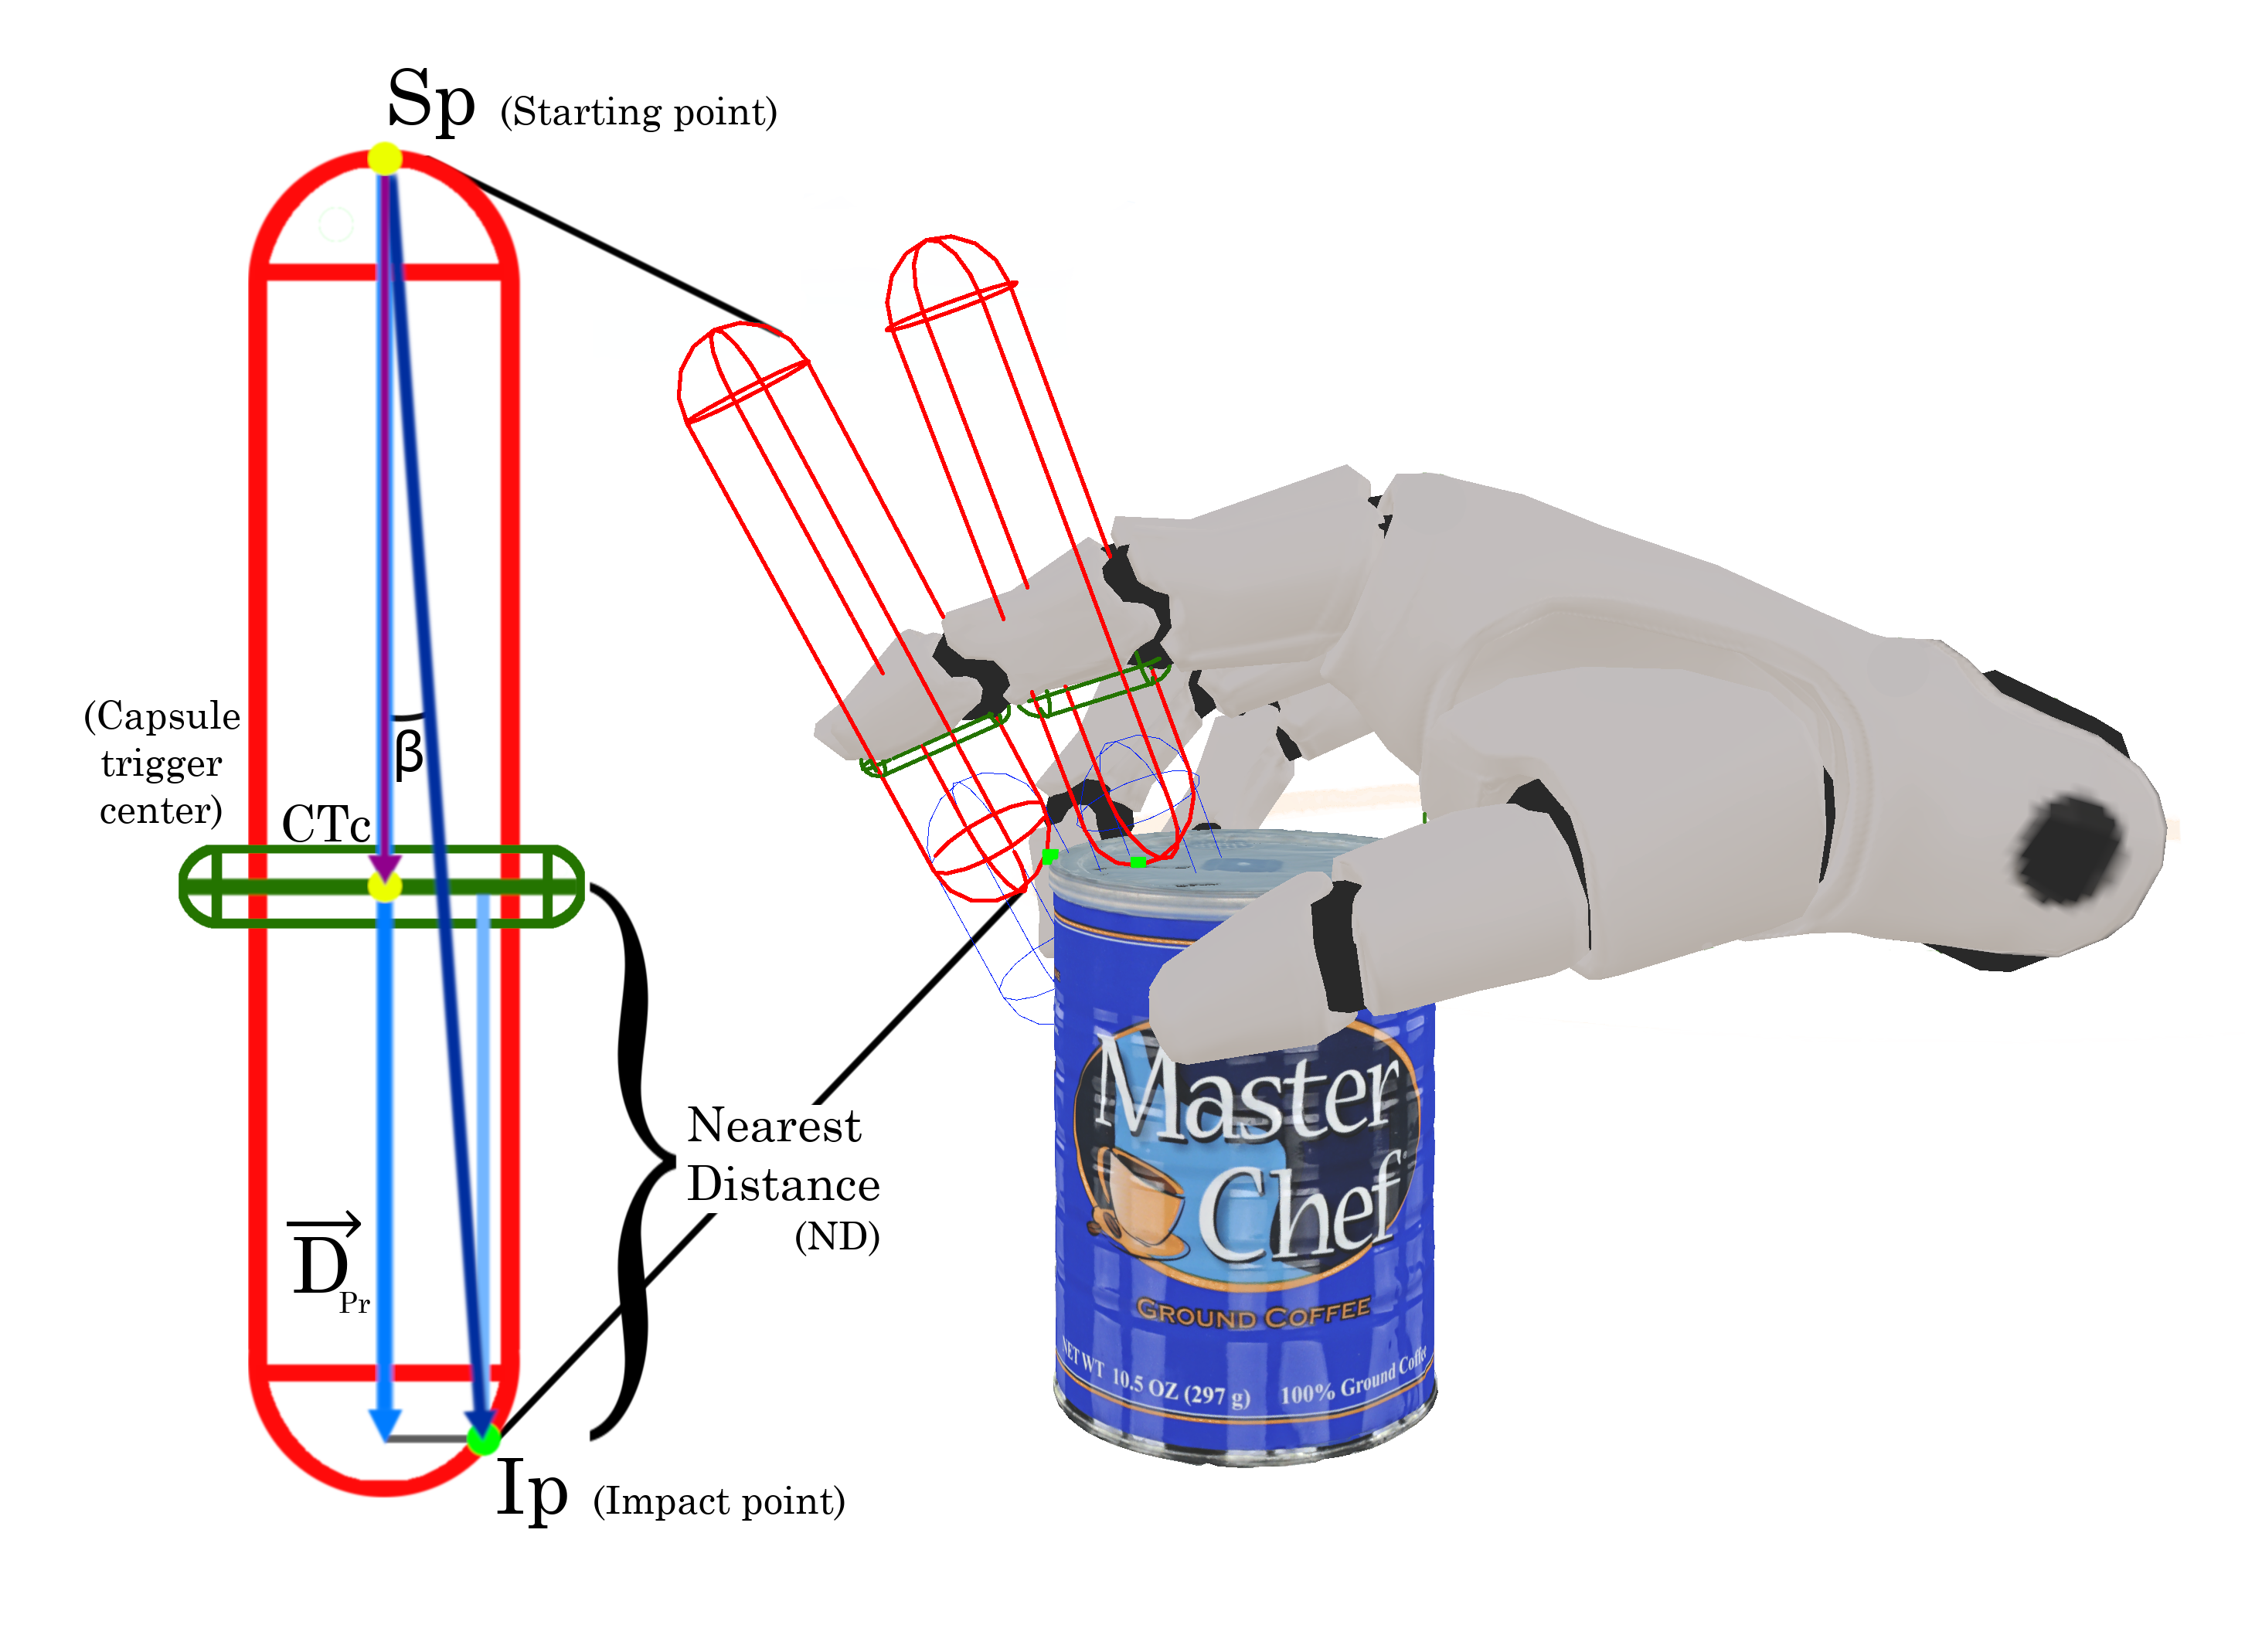
\includegraphics[width=0.70\textwidth]{figures/unrealgrasp/distanceCalculusMod.png}
	\caption{Distance computation for index finger.}
	\label{fig:distanceCalculus}
\end{figure}
The nearest distance computation is approximated by an equation that was developed to find the distance between the impact point, and the plane that contains the capsule trigger center point and is perpendicular to the longitudinal axis of the red capsule. Capsule triggers centers are located on the surface of the hand mesh, so this computation should approximate the nearest distance to the mesh well enough, without being computationally too demanding. To compute this distance, we define the following vectors from the three input points (the starting point of the red capsule, the impact point and the capsule trigger center point):
\begin{equation} \label{eq:1aux1}
\begin{split}
\overrightarrow{D_{Ip}} &= Ip - Sp\\
\overrightarrow{D_{CTc}} &= CTc - Sp
\end{split}
\end{equation}  
where $\overrightarrow{D_{Ip}}$ is the vector from the starting point to the impact point, and $\overrightarrow{D_{CTc}}$ vector represents the direction of the longitudinal axis of the red capsule. They are represented in navy blue and purple respectively in Figure \ref{fig:distanceCalculus}. Then, we find the cosine of the angle they form through their dot product:
\begin{equation} \label{eq:1aux2}
\begin{split}
\overrightarrow{D_{Ip}} \cdot \overrightarrow{D_{CTc}} &= |\overrightarrow{D_{Ip}}| * |\overrightarrow{D_{CTc}}| * cos(\beta)\\
cos(\beta) &= \frac{\overrightarrow{D_{Ip}} \cdot \overrightarrow{D_{CTc}}}{|\overrightarrow{D_{Ip}}| * |\overrightarrow{D_{CTc}}|}\\
\end{split}
\end{equation}
We can now substitute that cosine when computing the projection of $\overrightarrow{D_{Ip}}$ over the longitudinal axis of the red capsule ($\overrightarrow{D_{Pr}}$ in Figure \ref{fig:distanceCalculus}):
\begin{equation} \label{eq:1aux3}
\begin{split}
|\overrightarrow{D_{Pr}}| &= cos(\beta) * |\overrightarrow{D_{Ip}}|\\
|\overrightarrow{D_{Pr}}| &= \frac{\overrightarrow{D_{Ip}} \cdot \overrightarrow{D_{CTc}}}{|\overrightarrow{D_{CTc}}| * |\overrightarrow{D_{Ip}}|} * |\overrightarrow{D_{Ip}}|\\
|\overrightarrow{D_{Pr}}| &= \frac{\overrightarrow{D_{Ip}} \cdot \overrightarrow{D_{CTc}}}{|\overrightarrow{D_{CTc}}|}
\end{split}
\end{equation}
Having that module, we only have to subtract $|\overrightarrow{D_{CTc}}|$ in order to obtain the desired distance:  
\begin{equation} \label{eq:1}
\begin{split}
ND(Ip,Sp,CTc) &= \frac{\overrightarrow{D_{Ip}} \cdot \overrightarrow{D_{CTc}} }{|\overrightarrow{D_{CTc}}|} - |\overrightarrow{D_{CTc}}|\\
ND(Ip,Sp,CTc) &= \frac{\overrightarrow{Ip-Sp} \cdot \overrightarrow{CTc-Sp} }{|\overrightarrow{CTc-Sp}|} - |\overrightarrow{CTc-Sp}|
\end{split}
\end{equation}
Computing the distance like this, with this final subtraction, allows to obtain a positive distance when impact point is outside the hand mesh, and a negative one if it is inside.

We compute the nearest distance per each capsule trigger attached to a finger phalanx. As stated before, if the distance is negative, this indicates a finger penetration issue on the object surface. Otherwise, if distance is positive, it means that finger stopped above the object surface. The ideal case is when a zero distance is obtained, that is, the finger is perfectly situated on the object surface.

The total error for the hand is represented by the following equation:
\begin{equation} \label{eq:2}
HandError = \sum_{i=1}^{N_{Fingers}}\frac{\sum_{j=1}^{N_{CTF}}|ND(Ip_{ij},Sp_{ij},CTc_{ij})|}{N_{CapsuleTriggersPerFinger}}
\end{equation}


\subsection{Procedure}

The system performance analysis begins with the quantitative evaluation. In this first phase, the user will be embodied in a controlled scenario where 30 different objects will be spawned in a delimited area, with random orientation, and in the same order as represented in Figure \ref{fig:ycbgrasps}. The user will try to grasp the object as he would do in real life and as quickly as possible. For each grasping, the system will compute the error metric and will also store the time spent by the user in grasping the object. The purpose of this first phase is to visually analyze grasping quality which is directly related to user expertise in VR environments and concretely with our grasping system. An experienced user would know system limits both when interacting with complex geometries or with large objects that would make it difficult to perform the grasp action quickly and naturally.

For the qualitative evaluation, the same user will be embodied in a photorealistic scenario changing mannequin hands by human hand model with realistic textures. After interacting freely in the photorealistic virtual environment, the user will have to answer the evaluation questionnaire defined in Table \ref{table:questionnaire}. The main purpose is the evaluation of interaction realism, finger and hand movement naturalness and motor control, among other qualitative aspects regarding user experience in VR environments. 

Demo videos for both quantitative and qualitative evaluations are available at Github (\url{https://github.com/3dperceptionlab/unrealgrasp}).


\section{Results and discussion}
\label{sec:results}

In this section we are going to analyze the results obtained from the performance evaluation process represented in Figure \ref{chart:timeanderror}. On one hand, we will draw conclusions on the average time needed to grasp the objects for each user group (experienced and inexperienced) and all users as a whole. On the other hand, we will consider the average error obtained from the interaction with each object. In this way, we will be able to identify the most cumbersome objects to be manipulated, either by their geometry or size. In addition, we will contrast system performance between inexperienced and experienced users to analyze our system behavior with users without previous VR experience.


\subsection{Qualitative evaluation}

Qualitative evaluation for each participant was calculated using the Equation \ref{eq:6} obtaining a score for each qualitative aspect. In Table \ref{table:qualitativeresults} we represent for each group of participants: the average score for each evaluation aspect and the total embodiment score computed using the Equation \ref{eq:5}.

\begin{table}
	\resizebox{0.95\linewidth}{!}{
		\begin{tabular}{lcc}
			\hline
			& \multicolumn{2}{c}{Score} \\
			\cline{2-3}
			Evaluation Aspects    & Experienced users & Inexperienced users \\
			\hline
			(1) Motor Control     & 1.85    & 2.34      \\
			(2) Finger Movement Realism & 2.33   & 2.51       \\
			(3) Interaction Realism      & 1.84     & 1.95      \\
			\hline
			Embodiment score & 1.97 &  2.19 \\
			\hline
	\end{tabular}}
	\caption{Average score for each qualitative aspect of the evaluation and group of participants. Maximum result would be three. Results were obtained using the Equation \ref{eq:6}.}
	\label{table:qualitativeresults}
\end{table}

Regarding the represented results in Table \ref{table:qualitativeresults}, the evaluation of experienced users has been more disadvantageous as they have a more elaborated criterion given their previous experience with virtual reality applications. Finger movement realism (aspect 2) was evaluated similarly by both groups. This is because the hand closing and opening gestures are guided by the same animation in both cases. Finally, the reported results referring to the interaction realism have been the lowest in both cases. This is mostly because users cannot control their individual fingers movement, since general hand gesture is controlled by a unique trigger button of the controller. The average embodiment score computed using the Equation \ref{eq:5} is 2.08 (range of [-3,3]).

\begin{landscape}
	\begin{figure}
		\centering
		\begin{tikzpicture}[baseline]
		\begin{axis}[
		ybar= 0pt,
		xtick=data,
		symbolic x coords= {a,b,c,d,e,f,g,h,i,j,k,l,m,n,o,p,q,r,s,t,u,v,w,x,y,z,aa,ab,ac,ad},
		x tick label style={anchor=north},
		typeset ticklabels with strut,
		enlarge x limits=0.025,
		enlarge y limits=0.3,
		bar width=0.42 em,
		grid=both,
		grid style={line width=.1pt, draw=gray!10},
		major grid style={line width=.2pt,draw=gray!50},
		ylabel={Time [$s$]},
		ylabel near ticks,
		width=\linewidth,
		height=6cm,
		legend style={legend cell align=left, align=left, draw=white!15!black, legend columns= -1},
		legend pos=north west
		]
		\addplot[azure, fill=azure!40] table[x=object,y=0]{data/time_per_object.dat};
		\addplot[red, fill=red!40] table[x=object,y=1]{data/time_per_object.dat};
		\addplot[green, fill=green!40] table[x=object,y=0]{data/time_per_object_overall.dat};
		\legend{Experienced users, Inexperienced users, All users}
		\end{axis}
		\end{tikzpicture}
		
		\begin{tikzpicture}[baseline]
		\begin{axis}[
		ybar= 0pt,
		xtick=data,
		symbolic x coords= {a,b,c,d,e,f,g,h,i,j,k,l,m,n,o,p,q,r,s,t,u,v,w,x,y,z,aa,ab,ac,ad},
		x tick label style={anchor=north},
		typeset ticklabels with strut,
		enlarge x limits=0.025,
		enlarge y limits=0.05,
		bar width=0.42 em,
		grid=both,
		grid style={line width=.1pt, draw=gray!10},
		major grid style={line width=.2pt,draw=gray!50},
		ylabel={Error [$mm$]},
		xlabel={Object [$id$]},
		xlabel near ticks,
		ylabel near ticks,
		width=\linewidth,
		height=6cm, 
		legend style={legend cell align=left, align=left, draw=white!15!black, legend columns= -1},
		legend pos=north west
		]
		\addplot[azure, fill=azure!40] table[x=object,y=0]{data/accuracy_per_object.dat};
		\addplot[red, fill=red!40] table[x=object,y=1]{data/accuracy_per_object.dat};
		\addplot[green, fill=green!40] table[x=object,y=0]{data/accuracy_per_object_overall.dat};
		\legend{Experienced users, Inexperienced users, All users}
		\end{axis}
		\end{tikzpicture}
		\caption{Average time (top) needed to grasp each object and average error (bottom) of the performed grasps. The group of experienced users (i.e. users who had already used virtual reality technologies) is represented in blue, the group of inexperienced users (i.e. users without any previous experience with virtual reality environments) is represented in red, and finally the average time for all users is represented in green.}
		\label{chart:timeanderror}
	\end{figure}
\end{landscape}

\subsection{Quantitative evaluation}

As expected, inexperienced users have taken longer to grasp almost all the objects due to the lack of practice and expertise with the system. Analyzing Figure \ref{chart:timeanderror}, experienced users only have taken longer in grasping some tools such as, the flat screwdriver (Figure \ref{fig:flatscrewdriver}) and hammer (Figure \ref{fig:hammer}). Inexperienced users took an average of 0.36 seconds longer to grab the objects. In practice and regarding interaction, this is not a factor that is going to make a difference. Moreover, the tuna fish can (Figure \ref{fig:tunafishcan}), potted meat can (Figure \ref{fig:pottedmeatcan}), spatula (Figure \ref{fig:spatula}), toy airplane (Figure \ref{fig:toyairplane}) and bleach cleaner (Figure \ref{fig:bleachcleaner}) are the most time consuming when grasped by the users. This is mainly because of their sizes and complex geometries. Since objects are spawned with a random orientation and taking into account that, for example, the power drill (Figure \ref{fig:powerdrill}) and spatula have a handle, the time needed to grasp them can be variable and also related to the user VR skills. The user would unconsciously try to grasp the object by its handle, which would add some extra time depending on the orientation of the handle relative to the hand when the object is spawned. Even so, we can conclude that generally the largest objects are those that the user takes the longest to grasp.

Analyzing the average error obtained for each object, a similarity is observed between the results of inexperienced users and those experienced. The most significant differences were observed when manipulating the power drill and the spatula. This is because its complex geometries and large dimensions make it difficult to grasp (as in the case of toy airplane). Analyzing also the overall error, we come to the conclusion that the largest objects, such as the toy airplane, power drill, and bleach cleaner are those with the highest error rate. In addition, we observe how overall error decreases in time from the first object manipulated to the last. This is mainly because, user skills and expertise with the grasping system are improving progressively. On the basis of the obtained results, we can conclude that our solution is user-friendly, a fact that refers to a steep learning curve.


\section{Applications}
\label{sec:applications}

Our grasping system can be applied to several existing problems in different areas of interest, such as: robotics \cite{bric2016current}, rehabilitation \cite{levin2015emergence} and interaction using augmented reality \cite{lv2015touch}.

In robotics, different works have been explored to implement robust grasp approaches that allow robots to interact with the environment. These contributions are organized in mainly four different blocks \cite{bohg2014data}: methods that rely on known objects and previously estimated grasp points  \cite{lin2015robot}, grasping methods for familiar objects\cite{vahrenkamp2016part}, methods for unknown objects based on the analysis of object geometry \cite{zapata2017using} and automatic learning approaches\cite{levine2018learning}. Our approach is more closely related to this last block, where its use would potentially be a relevant contribution. As a direct application, our system enables human-robot knowledge transfer where robots try to imitate human behavior in performing grasping.

Our grasping system is also useful for rehabilitation of patients with hand motor difficulties, and it could even be done remotely assisted by an expert \cite {escobar2018virtual}, or through an automatic system \cite{avola2018vrheab}. Several works have demonstrated the viability of patient rehabilitation in virtual environments \cite{levin2015emergence}, helping them to improve the mobility of their hands in daily tasks \cite{faria2016benefits}. Our novel error metric in combination with other automatic learning methods, can be used to guide patients during rehabilitation with feedback information and instructions. This will make rehabilitation a more attractive process, by quantifying the patient progress and visualizing its improvements over the duration of rehabilitation.

Finally, our grasping system integrated in UnrealROX \cite{martinez2019} enables many other computer vision and artificial intelligence applications by providing synthetic ground truth data, such as depth and normal maps, object masks, trajectories, stereo pairs, etc. of the virtual human hands interacting with real objects from the YCB dataset.


\section{Limitations and future works}
\label{sec:limitationsfutureworks}
Our proposal has several major limitations:
\begin{itemize}
	\item Hand movement is based on a single animation regardless object geometry. Depending on the object shape we could vary grasping gesture: spherical-grasping, cylindrical-grasping, finger-pinch, key-pinch, etc. However, our grasping gesture was experimentally the best when dealing with different shaped objects. 
	\item The object can be grasped with only one hand. The user can interact with different objects using both hands at the same time. But not the same object with both hands. 
	\item Sometimes it is difficult to deal with large objects due to the initial hand posture or because objects slide out from the hand palm due to physical collisions. Experienced users can better deal with this problem.
\end{itemize}

As future work, and in order to improve our grasping system, we could vary the hand grip gesture according to the object geometry we are manipulating. This is finding a correspondence between object geometry and a simple shape, e.g. a tennis ball is similar to a sphere thus proceeding with a spherical grasp movement. At the application level, there are several possibilities as we discussed in the previous section. However, we would like to emphasize the use of contact points obtained when grasping an object in virtual reality, to transfer the human behavior to real robots.


\section{Conclusions}
\label{sec:conclusion}
This work proposes a flexible and realistic looking grasping system which enables smooth and real-time interaction in virtual reality environments with arbitrary shaped objects. This approach is not restricted by object geometry, is fully user-controlled, and is modular and easy to implement on different meshes or skeletal configurations. In order to validate our approach, an exhaustive evaluation process was carried out. Our system was evaluated qualitatively and quantitatively by two groups of participants: with previous experience in virtual reality environments (experienced users) and without expertise in VR (inexperienced). For the quantitative evaluation, a new error metric has been proposed to evaluate each grasp, quantifying hand-object overlapping. From the performance analysis results, we conclude that user overall experience was satisfactory and positive. Analyzing the quantitative evaluation, the error difference between experienced users and non experienced is subtle. Moreover, average errors are progressively smaller as more object are grasped. This clearly indicates a steep learning curve. In addition, the qualitative analysis points to a natural and realistic interaction. Users can freely manipulate previously defined dynamic objects in the photorealistic environment. Moreover, grasping contact points can be easily extracted, thus enabling numerous applications, especially in the field of robotics. Unreal Engine 4 project source code is available at GitHub alongside several video demonstrations (\url{https://github.com/3dperceptionlab/unrealgrasp}). This approach can easily be implemented on different game engines.
\chapter{Translating Synthetic Hands to the Real Domain}
\label{cha:synthtoreal}

\begin{chapterabstract}
We present \ac{HGAN}, a cycle-consistent adversarial learning approach implementing multi-scale perceptual discriminators. It is designed to translate synthetic images of hands to the real domain. Synthetic hands provide complete ground-truth annotations, yet they are not representative of the target distribution of real-world data. We strive to provide the perfect blend of a realistic hand appearance with synthetic annotations. Relying on image-to-image translation, we improve the appearance of synthetic hands to approximate the statistical distribution underlying a collection of real images of hands. \ac{HGAN} tackles not only the cross-domain tone mapping but also structural differences in localized areas such as shading discontinuities. Results are evaluated on a qualitative and quantitative basis, improving previous works. Furthermore, we relied on the hand classification task to claim our generated hands are statistically similar to the real domain of hands.
\end{chapterabstract}

\minitoc

\clearpage

\section{Introduction}
\label{cha:synthtoreal:sec:intro}
The lack of large amounts of high-quality annotated data is still a barrier for supervised deep learning approaches. Manual labeling is tedious and time-consuming, particularly when it comes to per-pixel or 3D annotations. For this reason, generating fully annotated and quasi-unlimited data from a controlled virtual environment emerged as a potential solution to data scarcity. Synthetic data generation, despite its recent success in different fields~\cite{Nikolaus2018,Garcia2018b,Hwang2020}, has at least two major flaws: i) it is challenging, if not impossible, to perfectly simulate real-world properties in a synthetic environment, and ii) training deep models exclusively on synthetic data (even if they are photorealistic) commonly exhibits generalization issues in the real domain. In the context of domain adaptation~\cite{Zhao2020}, these issues are addressed by reducing the domain distribution discrepancy between synthetic and real data. 

\vspace*{0.1cm}\noindent\textbf{Purpose:} We focus on changing the visual appearance of synthetically generated hands to approximate the statistical distribution underlying a collection of real images of hands. We focus on hands for two reasons: i) synthetic hands provide full ground-truth annotations, yet they are not representative of the target distribution of real-world data, and ii) large-scale datasets of real hands are sparsely labeled e.g. they lack 3D annotations. In this work, we want to translate synthetic hands to the real domain, preserving the hand shape to ensure the inter-domain ground truth correspondence (see Figure~\ref{fig:hands_teaser}).

\vspace*{0.1cm}\noindent\textbf{Our work:} For this purpose, we present the \ac{HGAN} architecture, a cycle-consistent adversarial learning approach~\cite{Zhu2017} implementing multi-scale perceptual discriminators~\cite{Sungatullina2018}. On the one hand, cycle-consistency makes the model learn the mapping between the two domains in an unsupervised fashion and from unpaired images. On the other hand, perceptual discriminators enforce cross-domain content and style transfer by learning statistics in a high-level feature space. Besides tone mapping, this synergy allows the model to hallucinate finer details (see Figure~\ref{fig:hair}) and remove artifacts such as shading discontinuities (see Figure~\ref{fig:artifacts}). This leads to an overall improvement in the appearance of the generated hands, which we assess on a qualitative and quantitative basis. Our model is closely related to~\cite{Mueller2018}, sharing the same goal as their \ac{GeoConGAN} model.

\vspace*{0.1cm}\noindent\textbf{Contributions:} First, we present an adversarial approach for unsupervised domain adaptation reducing the domain gap discrepancy between synthetic and real hands. Second, we show improvements over the proposed baseline~\cite{Mueller2018} on a qualitative and quantitative basis. Furthermore, relying on the hand classification task we claim our generated hands are statistically similar to the real domain of hands. Our source code is available at GitHub\footnote{\href{https://github.com/sergiuoprea/hgan}{https://github.com/sergiuoprea/hgan}}.

\section{Related Works}
\label{cha:synthtoreal:sec:relatedworks}
In this section we provide a brief overview of works on domain adaptation, perceptual losses and synthetic-to-real translation as they are related topics to our task at hand.

\vspace*{0.1cm}\noindent\textbf{Domain adaptation} aims to narrow the distribution discrepancy between a labeled source domain and an unlabeled or sparsely annotated target domain~\cite{Zhao2020}. Hoffman \textit{et al.} proposed the \ac{CyCADA} architecture~\cite{Hoffman2018}. To preserve semantic information in the distribution alignment process, they used a semantic task loss to enforce the cycle-consistency. Likewise, Tran \textit{et al.}~\cite{Tran2019} proposed an attribute-conditioned \ac{CycleGAN} generating multiple target images with different attributes e.g. day or night. Aiming to translate domain-invariant features, Li \textit{et al.}~\cite{Li2019} proposed a more computationally efficient approach than~\cite{Hoffman2018} reporting also better results. Baek \textit{et al.}~\cite{baek2020weakly} proposed a framework based on \acp{GAN} and mesh rendering, that adapts the hand-object domain to a hand-only domain, while it learns hand pose estimation. Rad \textit{et al.}~\cite{rad2018domain} using depth information, showed accurate hand pose estimation on RGB images. For a more in-depth insight, we recommend the reader to consider~\cite{Zhao2020} reviewing the recent progress on single-source unsupervised domain adaptation.

\vspace*{0.1cm}\noindent\textbf{Synthetic-to-real translation} is the task of domain adaptation from synthetic data to real data. Advances in this field have enabled the use of quasi-unlimited and fully labelled synthetically generated data in real-world tasks. Such tasks include vehicle re-identification~\cite{Lee2020}, depth estimation~\cite{Maximov2020}, and geometry estimation~\cite{PNVR2020}, among others. Closely related to our work, Mueller \textit{et al.}~\cite{Mueller2018} used a geometrically consistent \ac{CycleGAN} for the same goal of closing the gap between synthetic and real images of hands. Concretely, they have used the visually improved and fully annotated synthetic hands for the 3D hand tracking task.  Shrivastava \textit{et al.}~\cite{Shrivastava2017} proposed a refiner network to improve synthetically generated images of eyes. Likewise, Atapattu \textit{et al.}~\cite{Atapattu2019} addressed the same task. On the other side, deep image synthesis showed relevant progress for the task at hand. Sangkloy \textit{et al.}~\cite{Sangkloy2017} propose the Scribbler method, an adversarial autoencoder design to synthesize images from imperfect hand drawn sketches using sparse color scribbles. Chen and Koltun~\cite{Chen2017} showed in their work that given a semantic layout, their proposed model can synthesize photographic images. The network is trained in a supervised fashion on pairs of photographs and their corresponding semantic layouts.

\vspace*{0.1cm}\noindent\textbf{Perceptual losses} use activations of pretrained networks such as VGG~\cite{Simonyan2015} to train another network. Such features, extracted at different scales, represent not only low-level image details, but also global structure. This has fostered advances in image style transfer and super-resolution~\cite{Johnson2016,Wang2020}, texture synthesis~\cite{Ulyanov2016}, image inpainting~\cite{Su2019} and image autoencoder embeddings~\cite{Pihlgren2020}, to name a few. Perceptual losses have been widely used in supervised tasks, however in the unsupervised scenario their application is not direct because of the lack of input/target image pairs. In this regard, Wang \textit{et al.}~\cite{Wang2018} was the first to implement a multi-scale perceptual discriminator for the unsupervised image-to-image translation task. PerceptualGAN~\cite{Li2017} uses perceptual losses to narrow the representation difference between small and large-sized objects to improve small object detection. Correlating perceptual similarity between pairs of images with human perceptual judgement, Zhang \textit{et al.}~\cite{Zhang2018} found that activations extracted from intermediate layers of a classification network do indeed correspond to human perception.

\section{Method}
\label{cha:synthtoreal:cha:method}

\begin{figure}[!htb]
	\centering
	\includegraphics[width=\textwidth]{figures/synthtoreal/architecture.pdf}
	\caption{On the left, multi-scale perceptual discriminator using features, $F_i$, extracted at different scales from VGG network. At each scale, perceptual statistics are stacked after convolutional blocks (convolution + leakyReLU). On the right, our \ac{HGAN} model performing the inter-domain translation in both directions. On the one side, generators $G_r$ and $G_s$ perform the synthetic-to-real and real-to-synthetic translation, respectively. On the other side, discriminators learn the statistics underlying real ($D_r$) and synthetic ($D_s$) domains. The generators and discriminators are trained simultaneously, in an adversarial fashion. The representation of the perceptual discriminator was inspired by~\cite{Sungatullina2018}.}
	\label{fig:architecture}
\end{figure}

We introduce \acf{HGAN}, an image-to-image translation model dedicated to narrow the distribution discrepancy between synthetic and real images of hands. With this architecture, we opt to achieve the following objectives:
\begin{itemize}
	\item \emph{Learning a mapping between synthetic and real hands.} For this purpose, we rely on \acp{CycleGAN}~\cite{Zhu2017}. These architectures were specifically designed for the unsupervised image translation task given unpaired training data. Their main goal is the cross-domain transfer of low-level appearance such as color or texture while preserving high-level attributes such as content or geometric structure. Our model was built on \acp{CycleGAN} for two reasons: i)~we deal with unpaired data, since for a given image of a synthetic hand we lack its corresponding target image in the real domain and vice versa, and ii)~they excel at learning a consistent texture mapping between domains, a fact that helps preserve skin color in the translation. As a drawback, they also one-to-one map unrealistic artifacts from the synthetic domain.
	
	\item \emph{Improving the cross-domain transfer of higher-level details.}
	Synthetic hands sometimes present unrealistic lighting and shadows due to imprecise geometry, among other undesirable artifacts. Avoiding their transfer to the target domain is not straightforward. This behavior is reinforced by the per-pixel losses implemented in the vanilla~\acp{CycleGAN} discriminators. To mitigate this side effect, perceptual losses~\cite{Johnson2016} showed great potential guiding the learning process in the high-level feature space. This is, matching feature representations extracted from pretrained networks. In contrast to per-pixel losses, these features are robust and invariant to slight image deformations. Relying on high-level features, perceptual discriminators~\cite{Sungatullina2018} enforce a more precise cross-domain transfer of high-level attributes. Our model implements a perceptual discriminator striving for a consistent inter-domain mapping of high-level cues. This will reduce to some extent shading discontinuities (see Figure~\ref{fig:artifacts}) and makes the model hallucinate content from the source domain such as hair (see Figure~\ref{fig:hair}).
\end{itemize}

\subsection{HandGAN Model}
\ac{HGAN} is built on \acp{CycleGAN}~\cite{Zhu2017}, and implements multi-scale perceptual discriminators~\cite{Sungatullina2018} to enhance the translation of high-level appearance cues. Our model improves results compared to a state-of-the-art work \cite{Mueller2017}. Its architecture is depicted in Figure~\ref{fig:architecture}.

\vspace*{0.1cm}\noindent\textbf{Using \acp{CycleGAN}}: These models were designed for the unsupervised image-to-image translation task with unpaired data. They consist of two generators and discriminators (one generator and discriminator per domain) trained in an adversarial fashion. While generators perform the inter-domain translation, discriminators supervise their learning process based on the internal representation learned from each domain. The goal is to make generated data follow the underlying distribution of the target domain so as to fake discriminators.
\begin{figure}[!htb]
	\centering
	\includegraphics[width=\textwidth]{figures/synthtoreal/artifacts.pdf}
	\caption{Top row, synthetic hands. Bottom row, translated hands to the real domain. Notice how the perceptual discriminator drives the generator to treat shading discontinuities at the wrist, which are not found in real data.}
	\label{fig:artifacts}
\end{figure}

\vspace*{0.1cm}\noindent\textbf{Inspiration by \ac{GeoConGAN}}: On top of \ac{CycleGAN} architecture, \ac{GeoConGAN} implements a geometrically-consistent loss designed to preserve the shape of the hand in the translation. This is the binary cross-entropy between the hand shape in the source and target domains. For this purpose, it uses a pretrained network (SilNet) to segment the shape of a hand. This prevents the implementation of \ac{GeoConGAN} as an end-to-end network, leading to additional memory overhead. The advantages of the SilNet are clear when datasets do not provide hand segmentation masks. However, its usefulness is an open question as \acp{CycleGAN} inherently preserve structure during the translation using the cycle and identity losses. If hand segmentation masks are provided, these could be used in the loss function or to mask generator's outputs as we do in our models.

\vspace*{0.1cm}\noindent\textbf{Multi-scale perceptual discriminator}: Our approach is to implement a multi-scale perceptual discriminator based on feature representations extracted at different scales from a pretrained VGG16 net~\cite{Simonyan2015}. Following the original implementation~\cite{Sungatullina2018}, it consists of stacking learnable convolutional blocks used to process activations extracted at different scales from the VGG-16. Multi-scale representations help the model to learn from data represented at different levels of abstraction, enforcing the inter-domain mapping of both low-level and high-level features.
\begin{figure}[!htb]
	\centering
	\includegraphics[width=\textwidth]{figures/synthtoreal/hair.pdf}
	\caption{Top row, real hands. Bottom row, hands translated to the synthetic domain. Notice how the perceptual discriminator makes the generator to hallucinate hair in the synthetic domain.}
	\label{fig:hair}
\end{figure}

\subsection{Implementation}

\vspace*{0.1cm}\noindent\textbf{Building blocks:} We have used the building blocks implemented in the \ac{CycleGAN} architecture. \ac{CycleGAN} implements PatchGAN-like~\cite{Isola2017} discriminators designed to map the input images to square patches. These discriminators learn the statistics at a patch-level, leveraging their effective receptive field. They aim to classify whether overlapping image patches come from the real or synthetic domain. As an alternative, PixelGAN ($1 \times 1$ PatchGAN) discriminators perform a per-pixel decision and in some tasks showed an enhanced diversity in generated data. On the generator side, the predominant models are ResNet-based~\cite{He2016}. We have considered both patch and pixel-based discriminators alongside generators featuring 4, 6, and 9 residual blocks.

\vspace*{0.1cm}\noindent\textbf{Multi-scale perceptual discriminator:} It was implemented as a PatchGAN-based model and considers representations extracted at different output scales (multi-scale). Concretely, our discriminator classifies their inputs using overlapping square patches of 16, 8 and 4 sizes. This makes the learning process focus from the lowest-level to the higher-level image cues. Different from~\cite{Sungatullina2018}, we rely on VGG-16~\cite{Simonyan2015} to extract activations at four different scales.

\subsection{Loss functions}
Let $R$ and $S$ be the real and synthetic domains of hand images where $r_i\in R$ and $s_i\in S$ are samples from each domain. We denote the data distribution as $\boldsymbol{r} \sim p_{\mathrm{data}}(\boldsymbol{r})$ and $\boldsymbol{s} \sim p_{\mathrm{data}}(\boldsymbol{s})$. On the one side, the goal is to make generators $G_s$ and $G_r$ learn two mappings $G:R\to S$ and $F:S\to R$, respectively. On the other side, discriminator $D_r$ discriminates between image $r_i$ and translated image $F(s_i)$; likewise, discriminator $D_s$ aims to distinguish between $s_i$ and $G(r_i)$. Generators and discriminators are trained simultaneously, in an adversarial fashion. 

Following the recommendations in the original \ac{CycleGAN}, we have used the least-squares loss\cite{Mao2017} to stabilize training. For instance, generator $G_s$ and discriminator $D_s$ are trained as follows:
\begin{equation}\begin{aligned}
\mathcal{L}_{\mathrm{GAN}}\left(D_{S}, R, S\right) &=\frac{1}{2} \mathbb{E}_{\boldsymbol{s} \sim p_{\text{data}}(\boldsymbol{s})}\left[(D_{S}(\boldsymbol{s})-1)^{2}\right] \\
&+\frac{1}{2} \mathbb{E}_{\boldsymbol{r} \sim p_{\boldsymbol{\text{data}}}(\boldsymbol{r})}\left[(D_{S}(G_{S}(\boldsymbol{r})))^{2}\right] \\
\mathcal{L}_{\mathrm{GAN}}\left(G_{S}, R, S\right)  &= \frac{1}{2}\mathbb{E}_{\boldsymbol{s} \sim p_{\boldsymbol{s}}(\boldsymbol{s})}\left[(D_{S}(G_{S}(\boldsymbol{r}))-1)^{2}\right]
\end{aligned}\end{equation}

In the case of the multi-scale perceptual discriminators, their inputs are features extracted from the VGG network at four different scales. Moreover, the outputs of the discriminator are also at multiple scales. Formally, $D_{S}(s)$ and $D_{S}(G_{S}(r))$ output vectors $Y$ and $Z$ of $n$ elements where $n$ is the total number of output scales. Under this configuration, $\mathcal{L}_{\mathrm{GAN}}\left(D_{S}, R, S\right)$ loss is computed as $\sum_{i=1}^{n}\frac{1}{2}\left(Y_{i}-1\right)^{2} + \frac{1}{2}\left(Z_{i}\right)^{2}$. Regarding cycle consistency and identity losses, we have used the implemented in the original \ac{CycleGAN}~\cite{Zhu2017}.

\section{Results}
\begin{figure}[!htb]
	\centering
	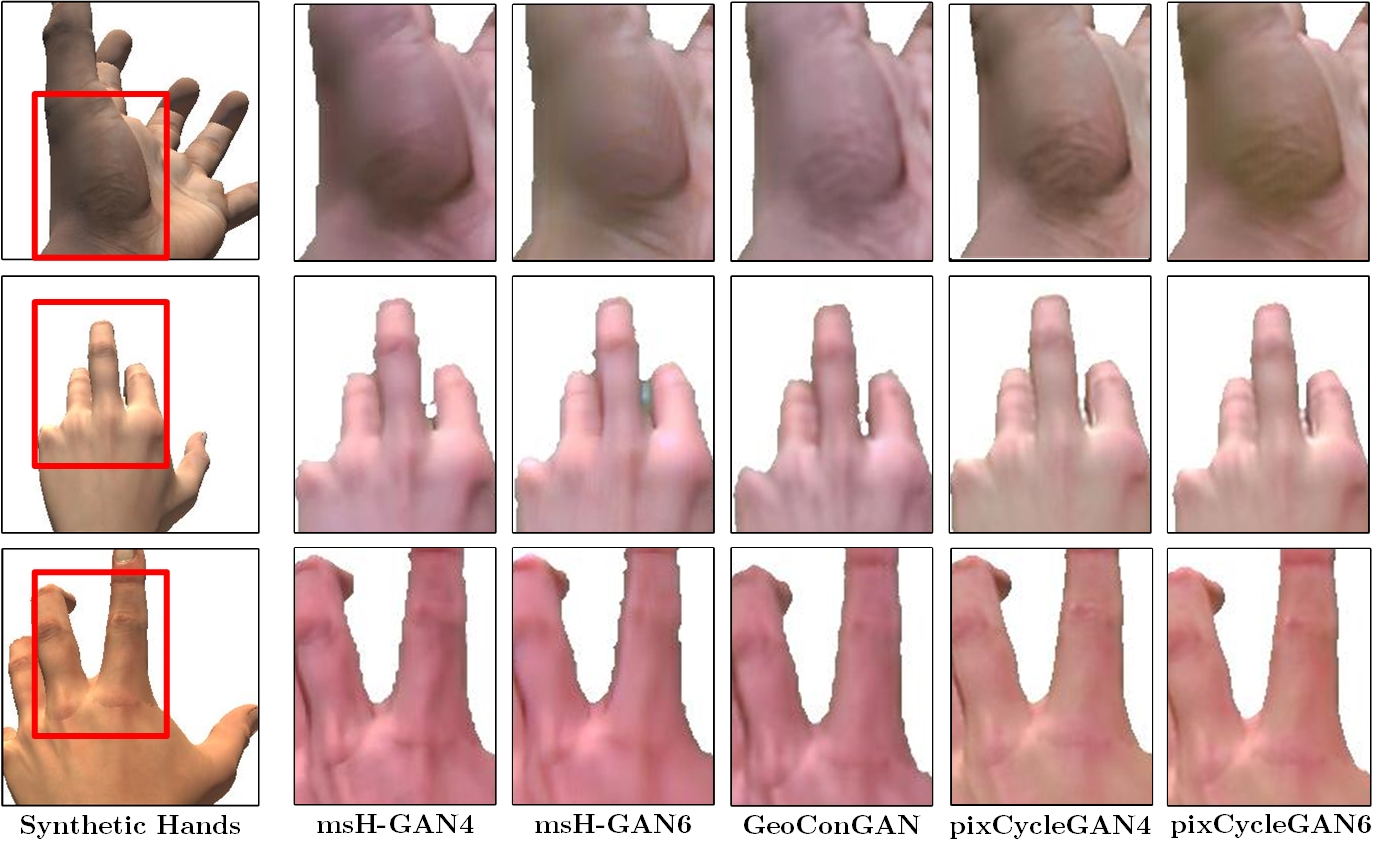
\includegraphics[width=0.95\textwidth]{figures/synthtoreal/hands_details.jpg}
	\caption{Generated images with our proposed architectures and the \ac{GeoConGAN} baseline. Notice how different are the outputs in terms of sharpness (top row), hand shape preservation (middle row) and skin color consistency (bottom row).}
	\label{fig:hand_details}
\end{figure}

In this section we define the model selection methodology and the evaluation procedure. Once selected, the best performing model configurations will be analyzed on a qualitative and quantitative basis. The qualitative evaluation consists of a visual inspection of the generated images in terms of skin color mapping realism, high-level details transfer and artifact presence. Furthermore, results will be compared with the baseline method using perceptual metrics.

\subsection{Implemented models and training details}
At the architectural level we have tested different generator/discriminator combinations. We varied the number of residual blocks in the generators and the discriminator type (patch, pixel and perceptual). Regarding the multi-scale perceptual discriminators we use outputs at different scales, concretely, squared patches of 16, 8 and 4 size. The implemented models are the following:
\begin{itemize}
	\item \textbf{\ac{GeoConGAN}}~\cite{Mueller2018}. Baseline model with a patch discriminator and a ResNet generator with 9 residual blocks.
	\item \textbf{pixCycleGAN4}. Implements a ResNet generator with 4 residual blocks and a pixel discriminator.
	\item \textbf{pixCycleGAN6}. Different from pixCycleGAN4 it uses 6 residual blocks in the generator.
	\item \textbf{msH-GAN4}. Features a multi-scale perceptual discriminator and a ResNet with 4 residual blocks.
	\item \textbf{msH-GAN6}. Different from msH-GAN4, it uses 6 residual blocks in the generator.
\end{itemize}

To select the best performing models, an exhaustive testing with different hyperparameter configurations was carried out. We explored different: learning rates, identity loss scale factor to seek for the best diversity/fidelity ratio in the generated data, image sizes for training and validation, and training batch size, among others.

\vspace*{0.1cm}\noindent\textbf{Baseline:} \ac{GeoConGAN} model is the latest work developed for the task at hand. Therefore, it is the baseline for our \ac{HGN} model for comparison purposes. \ac{GeoConGAN} was trained following the original implementation details~\cite{Mueller2018}. For the unspecified hyperparameters, we have used the default \ac{CycleGAN} configuration. Concretely, it is based on a Resnet generator with 9 residual blocks and a patch discriminator, both trained with a learning rate of $0.0002$. As a difference, our models do not rely on their hand shape-based loss. We directly use the provided masks in the dataset (with a previous pre-processing to remove noise and artifacts) to mask the generated images. 

\vspace*{0.1cm}\noindent\textbf{Training details:} All the models were trained with random cropped input images of $128\times128$ size and validated on bigger images of $256\times256$ using the \ac{FID} metric. Discriminators and generators were trained with a $0.00005$ learning rate on the whole datasets for 10 epochs. Networks were initialized using Xavier. Regarding weighted losses, we have used $0.5$ and $10$ weights for the identity loss and cycle loss, respectively. No learning rate schedulers were used. All the models were implemented using PyTorch Lightning framework and trained on NVIDIA TITAN Xp/V GPUs.

\subsection{Evaluation procedure}
We conducted an in-depth model search procedure to identify the best hyperparameter configurations. As a first step, a visual inspection of the results was carried out to broadly prune the less promising configurations. The fine-grain selection was performed validating the models using the \ac{FID} metric. Once training is completed, a quantitative evaluation is performed on the test set (2000 images) using the \ac{FID} and \ac{KID} metrics.

\vspace*{0.1cm}\noindent\textbf{Metrics:} Performance evaluation of generative models is challenging~\cite{Shmelkov2018,Xu2018} because of the lack of an explicit likelihood measure. Visual inspection to evaluate generated data quality is still a de facto evaluation protocol in the domain adaptation literature. However, some perceptual metrics such as \ac{FID}~\cite{Heusel2017} and \ac{KID}~\cite{Binkowski2018} were used as ad-hoc metrics correlated with the quality of the generated images. Particularly, \ac{FID} compares Gaussian statistics computed from activations (extracted from Inception V3 network) between the generated images and a bunch of samples from the target distribution. Conversely, to \ac{FID}, \ac{KID} serves as an unbiased evaluation metric. Since both metrics are mere statistical approximations to the true difference, they guarantee no correlation with performance on real-world tasks~\cite{Shmelkov2018}. However, they empirically demonstrated their usefulness in quantitative evaluations. Therefore, our quantitative analysis stands on these two metrics.

\vspace*{0.1cm}\noindent\textbf{Datasets}: For training and validation we have used the SynthHands~\cite{Mueller2017} and RealHands~\cite{Mueller2018} datasets. The former provides synthetically generated images from an egocentric view. It contains fully annotated images of male and female hands, both with and without object interaction. However, hand textures show undesirable artifacts and uncanny lighting or skin color. From the real domain, the RealHands dataset provides hand images of 7 different subjects with different skin tones and hand shapes. They were captured using a low-resolution webcam on a green-screen setup. Under this configuration, some images and their segmentation masks are blurry and contain strange artifacts. To use the masks in our models, we have refined them as follows. First, we reduced speckle noise using median filtering. Next, we addressed artifacts by searching for contours in the masks and removing those of a smaller area, assuming the hand is the biggest contour. Finally, we performed morphological operations such as closing, to fill some gaps in the hand mask, and erosion to remove residual background pixels on the hand border.

\subsection{Qualitative and quantitative analysis}
\begin{table}[!tb]
	\centering
	\ra{1.0}
	\caption{Perceptual metrics evaluating the implemented models. The msH-GAN4 and msH-GAN6 models obtained better results compared to the \ac{GeoConGAN} baseline and vanilla \acp{CycleGAN}.}
	\label{table:models}
	\resizebox{0.6\textwidth}{!}{
		\begin{tabular} {@{}lcc@{}} 
			\toprule
			\textbf{method} & \textbf{FID}$\downarrow$ & \textbf{KID}$\downarrow$ \\
			\midrule
			pix\ac{CycleGAN}6 & $71.639$ & $0.0530\pm0.0065$ \\
			pix\ac{CycleGAN}4 & $70.815$ & $0.0517\pm0.0065$ \\
			\ac{GeoConGAN} & $66.786$ & $0.0481\pm0.0065$ \\
			ms\ac{HGAN}4 & $63.297$ & $\mathbf{0.0479\pm0.0067}$ \\
			ms\ac{HGAN}6 & $\mathbf{63.185}$ & $0.0480\pm0.0066$ \\
			\bottomrule
	\end{tabular}}
\end{table}

The qualitative and quantitative evaluation was performed on the test set containing 2000 images of hands. First, a rough visual inspection was performed to determine the overall consistency in the skin color mapping over the whole test set. In this regard, perceptual-based approaches have shown greater consistency. This means that the generated hands are in general of a higher visual quality showing more similarities in the skin color with the real images of hands. On the other hand, approaches using pixel discriminators (pixCycleGAN4 and pixCycleGAN6) reported sharper hands (see top row in Figure~\ref{fig:hand_details}) and a more consistent hand shape preservation in the translation. The latter was detected by inspecting the small gaps between hand fingers (see middle row in Figure~\ref{fig:hand_details}). In this regard, pixel discriminators are helpful since they make the decision at the pixel-level. However, they also tend to one-to-one map the synthetic skin tone and geometry artifacts to the real domain. As we can observe in Figure~\ref{fig:hand_details}, the differences are noteworthy. This difference is also reflected in both \ac{FID} and \ac{KID} metrics, reporting worse quantitative results.

On the other side, PatchGAN-based discriminators tend to fill the tiny gaps between hand fingers (see msH-GAN6, middle row sample in Figure~\ref{fig:hand_details}). To combat this side effect, the \ac{GeoConGAN} architecture relies on a UNet network (called SilNet) to segment the hand shape which is then used in their geometrically consistent loss function. However, the differences with the msH-GAN4 model in terms of hand shape preservation are not clear. The latter uses the preprocessed hand masks which are applied to the generated images instead of an external architecture. This makes the model end-to-end and more parameter efficient, avoiding the extra memory overhead.

Quantitatively, perceptual-based approaches reported better results than the \ac{GeoConGAN}~\cite{Mueller2018} model. However, very subtle differences were noticed on the \ac{KID} metric. Furthermore, we claim that, for the problem at hand, the difference in the number of residual blocks in the generators has no major relevance to performance. Overall, the best performing methods were the msH-GAN4 and msH-GAN6 models. However, msH-GAN4 presented sharper results, subtle differences in skin color (visually more similar to the real hands) and was also less prominent in filling the gaps between fingers.

\subsection{A note on cross-domain similarity}
\begin{figure}[!t]
	\centering
	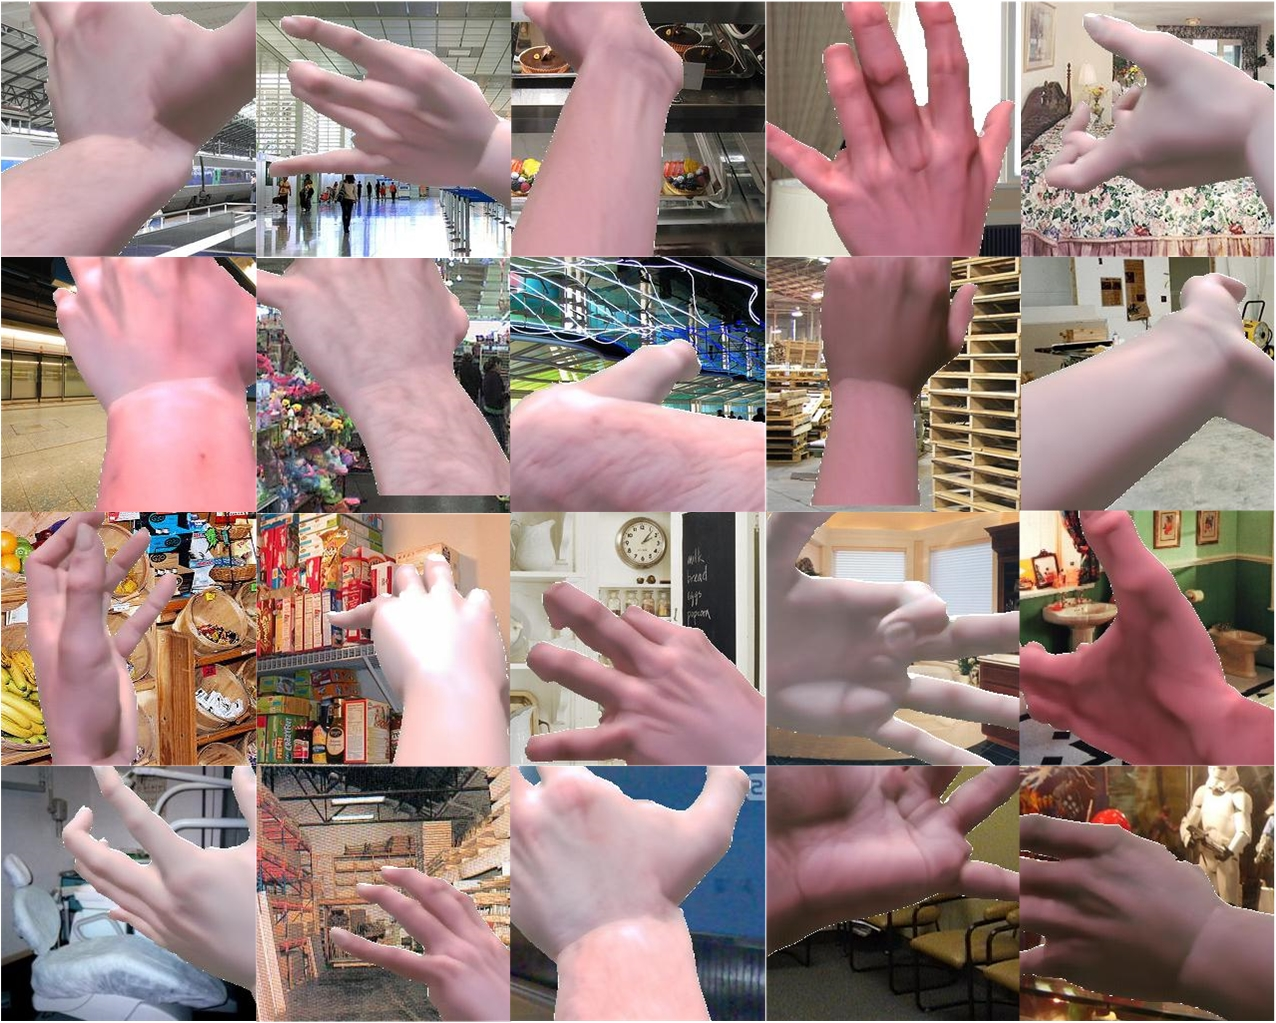
\includegraphics[width=\textwidth]{figures/synthtoreal/hands_application.jpg}
	\caption{Samples of the generated hands used in the classification task. Hands were generated using our \mbox{msH-GAN6} model and placed on random backgrounds extracted from~\cite{Quattoni2009}.}
	\label{fig:hand_application}
\end{figure}
\begin{table*}[!htb]
	\centering
	\ra{1.1}
	\caption{Evaluation of the \acs{VIT} model trained for binary classification (synthetic or real) and tested with synthetic (syn), real (rea) and generated (gen) hands. For training, we assume real and generated hands belong to the same class (real). Notice both classes were classified indistinguishably reporting slight differences in the metrics. $\|$ denotes separation between classes.}
	\label{table:test1}
	\resizebox{\textwidth}{!}{
		\begin{tabular} {@{}lllcccc@{}} 
			\toprule
			\textbf{$\#$} & \textbf{train set} & \textbf{test set} & \textbf{precision}$\uparrow$ & \textbf{recall}$\uparrow$ & \textbf{f1-score}$\uparrow$ & \textbf{accuracy}$\uparrow$ \\
			\midrule
			1 & syn $\|$ rea & syn $\|$ rea & $94.51\,\|\,97.38$ & $97.46\,\|\,94.34$ & $95.96\,\|\,95.84$ & $95.90$ \\
			& & syn $\|$ gen & $95.62\,\|\,97.18$ & $97.23\,\|\,95.54$ & $96.42\,\|\,96.35$ & $96.39$ \\
			\midrule
			2 & syn $\|$ gen & syn $\|$ rea & $95.29\,\|\,92.65$ & $92.43\,\|\,95.43$ & $93.84\,\|\,94.02$ & $93.93$ \\
			& & syn $\|$ gen & $98.91\,\|\,93.60$ & $93.23\,\|\,98.97$ & $95.98\,\|\,96.21$ & $96.10$\\
			\midrule
			3 & syn $\|$ (\textonehalf\,rea, \textonehalf\,gen) & syn $\|$ rea & $94.83\,\|\,96.96$ & $97.03\,\|\,94.71$ & $95.92\,\|\,95.82$ & $95.87$ \\
			& & syn $\|$ gen & $97.25\,\|\,97.15$ & $97.14\,\|\,97.26$ & $97.20\,\|\,97.20$ & $97.20$\\
			\bottomrule
	\end{tabular}}
\end{table*}

We rely on the hand classification task to claim our generated hands are statistically similar to the real domain of hands. We assume generated and real hands approximate a similar distribution if a classifier: (a) without being trained on generated hands, classifies most of them as real hands, and (b) confuses real with generated hands and vice versa, when learning to discriminate between them. We use metrics such as precision, recall, f1-score and accuracy, along with a confusion matrix showing the number of misclassified images, to analyze how similar is our generated data to the real domain of hands.

For (a), we have trained the \acf{VIT}~\cite{Dosovitskiy2020} model to distinguish between synthetic and real images of hands. Without the model knowing what a generated hand looks like, the goal is to classify the generated images and determine to which class (synthetic or real) they belong. We assume that if most of the generated images are classified as real hands, they approximate a similar distribution. Three different training sets with equal contribution per class were used in this first experiment:
\begin{enumerate}
	\item $10.500$ synthetic and $10.500$ real images.
	\item $10.500$ synthetic and $10.500$ generated images.
	\item $10.500$ synthetic and a combination of $5.250$ real and $5.250$ generated images representing the real hand class.
\end{enumerate}
The real and generated images were classified as real hands with similar precision in all tested scenarios (see Table~\ref{table:test1}). Furthermore, the use of a combination of generated and real images in the training set showed better results in classifying the generated images, while maintaining similar performance in classifying real hands.
\begin{table}[!tb]
	\centering
	\ra{1.1}
	\caption{Evaluation of the \acs{VIT} model trained on synthetic, real and generated images of hands ($10.500$ images per class). Notice how the model precisely classifies the synthetic hands, while confuses the real and generated classes reporting lower precision, recall and f$1$-score.}
	\label{table:test2}
	\resizebox{0.6\textwidth}{!}{
		\begin{tabular} {@{}lccc@{}} 
			\toprule
			\textbf{class} & \textbf{precision}$\uparrow$ & \textbf{recall}$\uparrow$ & \textbf{f1-score}$\uparrow$\\
			\midrule
			synthetic & $0.9540$ & $0.9546$ & $0.9543$ \\ 
			real & $0.7930$ & $0.8329$ & $0.8124$ \\
			generated & $0.8468$ & $0.8037$ & $0.8247$ \\
			\midrule
			\midrule
			\textbf{accuracy} & & & 0.8637 \\
			\bottomrule
	\end{tabular}}
\end{table}

But, what if we consider the generated hands belong to a different class? For (b) we want the \ac{VIT} model to learn the differences between real and generated hands. Note that the generated and synthetic hands have the same shape, but a different appearance. This shape correspondence overcomplicates the classification task and makes the \ac{VIT} model focus on the appearance of the hand rather than its shape. Assuming that the generated and real hands share similarities at a distribution level, the model should confuse these two classes, i.e. misclassify a generated hand as real and vice versa. We show the number of misclassified samples in the confusion matrix (see Figure~\ref{fig:confusion}) and the model performance in terms of precision, recall and f$1$-score in Table~\ref{table:test2}. The \ac{VIT} model precisely ($95.40\%$) classifies the synthetic hands, yet it confuses the generated with the real hands and vice versa. Concretely, $647$ ($18\%$) of the real hands were classified as generated and $465$ ($13\%$) of the generated hands as real. The misclassification has a direct impact on the per-class precision, recall and f$1$-score revealing the similarities between the generated and real hands.

Models were trained for $20$ epochs with a learning rate of $0.00001$ and tested with $3.500$ samples per class. For more implementation details, see the code repository.

\begin{figure}[!t]
	\centering
	\resizebox{.6\textwidth}{!}{\def\myConfMat{{
{3341,  121,   40},  %row 1
{ 114, 2915,  647},  %row 2
{  45,  465, 2813},  %row 3
}}

\def\classNames{{"syn","rea","gen"}} %class names. Adapt at will

\def\numClasses{3} %number of classes. Could be automatic, but you can change it for tests.

\def\myScale{1.5} % 1.5 is a good scale. Values under 1 may need smaller fonts!
\begin{tikzpicture}[
    scale = \myScale,
    %font={\scriptsize}, %for smaller scales, even \tiny may be useful
    ]

\tikzset{vertical label/.style={rotate=90,anchor=east}}   % usable styles for below
\tikzset{diagonal label/.style={rotate=45,anchor=north east}}

\foreach \y in {1,...,\numClasses} %loop vertical starting on top
{
    % Add class name on the left
    \node [anchor=east] at (0.4,-\y) {\pgfmathparse{\classNames[\y-1]}\pgfmathresult}; 
    
    \foreach \x in {1,...,\numClasses}  %loop horizontal starting on left
    {
%---- Start of automatic calculation of totSamples for the column ------------   
    \def\totSamples{0}
    \foreach \ll in {1,...,\numClasses}
    {
        \pgfmathparse{\myConfMat[\ll-1][\x-1]}   %fetch next element
        \xdef\totSamples{\totSamples+\pgfmathresult} %accumulate it with previous sum
        %must use \xdef fro global effect otherwise lost in foreach loop!
    }
    \pgfmathparse{\totSamples} \xdef\totSamples{\pgfmathresult}  % put the final sum in variable
%---- End of automatic calculation of totSamples ----------------
    
    \begin{scope}[shift={(\x,-\y)}]
        \def\mVal{\myConfMat[\y-1][\x-1]} % The value at index y,x (-1 because of zero indexing)
        \pgfmathtruncatemacro{\r}{\mVal}   %
        \pgfmathtruncatemacro{\p}{round(\r/\totSamples*100)}
        \coordinate (C) at (0,0);
        \ifthenelse{\p<50}{\def\txtcol{black}}{\def\txtcol{white}} %decide text color for contrast
        \node[
            draw,                 %draw lines
            text=\txtcol,         %text color (automatic for better contrast)
            align=center,         %align text inside cells (also for wrapping)
            fill=black!\p,        %intensity of fill (can change base color)
            minimum size=\myScale*10mm,    %cell size to fit the scale and integer dimensions (in cm)
            inner sep=0,          %remove all inner gaps to save space in small scales
            ] (C) {\r\\\p\%};     %text to put in cell (adapt at will)
        %Now if last vertical class add its label at the bottom
        \ifthenelse{\y=\numClasses}{
        \node [] at ($(C)-(0,0.75)$) % can use vertical or diagonal label as option
        {\pgfmathparse{\classNames[\x-1]}\pgfmathresult};}{}
    \end{scope}
    }
}
%Now add x and y labels on suitable coordinates
\coordinate (yaxis) at (-0.5,0.6-\numClasses/2);  %must adapt if class labels are wider!
\coordinate (xaxis) at (0.5+\numClasses/2, -\numClasses-1.15); %id. for non horizontal labels!
\node [vertical label] at (yaxis) {Predicted Class};
\node []               at (xaxis) {True Class};
\end{tikzpicture}}
	\caption{Confusion matrix representing the number of mislabeled samples among the different classes: synthetic (syn), real (rea), and generated (gen). Notice the confusion between the real and generated classes. $18\%$ of real hands were classified as generated, and $13\%$ of generated hands as real.}
	\label{fig:confusion}
\end{figure}

\section{Conclusions}
Despite the wealth of approaches in the domain adaptation field, methods addressing the synthetic-to-real translation of hands are few. On this line, we proposed the \ac{HGAN} model aiming to provide the perfect blend of a realistic hand appearance with synthetic annotations. We showed our \ac{HGAN} tackles not only inter-domain tone mapping but also hallucinates finer details. After an exhaustive model selection procedure, we reported comparable results to previous approaches on a qualitative and quantitative basis. We outperformed the \ac{GeoConGAN}~\cite{Mueller2018} model on \ac{FID} and \ac{KID} metrics. Furthermore, the generated data was used in a classification network demonstrating its usefulness in real-world applications.

\chapter{Video Prediction}
\label{cha:videoprediction}

\begin{chapterabstract}
The ability to predict, anticipate and reason about future outcomes is a key component of intelligent decision-making systems. In light of the success of deep learning in computer vision, deep-learning-based video prediction emerged as a promising research direction. Defined as a self-supervised learning task, video prediction represents a suitable framework for representation learning, as it demonstrated potential capabilities for extracting meaningful representations of the underlying patterns in natural videos. Motivated by the increasing interest in this task, we provide a review on the deep learning methods for prediction in video sequences. We firstly define the video prediction fundamentals, as well as mandatory background concepts and the most used datasets. Next, we carefully analyze existing video prediction models organized according to a proposed taxonomy, highlighting their contributions and significance in the field. The summary of the datasets and methods is accompanied with experimental results that facilitate the assessment of the state of the art on a quantitative basis. The paper is summarized by drawing some general conclusions, identifying open research challenges and by pointing out future research directions.
\end{chapterabstract}

\minitoc

\clearpage

\section{Introduction}
\label{cha:videoprediction:sec:introduction}

Will the car hit the pedestrian? That might be one of the questions that comes to our minds when we observe Figure~\ref{fig:pedestrian}. Answering this question might be in principle a hard task; however, if we take a careful look into the image sequence we may notice subtle clues that can help us to predict into the future, e.g., the person's body indicates that he is running fast enough, so he will be able to escape the car's trajectory. This example is just one situation among many others in which predicting future frames in video is useful.

\begin{figure}[!hbt]
	\centering
	\resizebox{0.75\textwidth}{!}{
		\begin{tikzpicture}
\node[inner sep=0.8pt, draw=blue!70, line width=0.05cm] (frame0) at (0,0)
    	{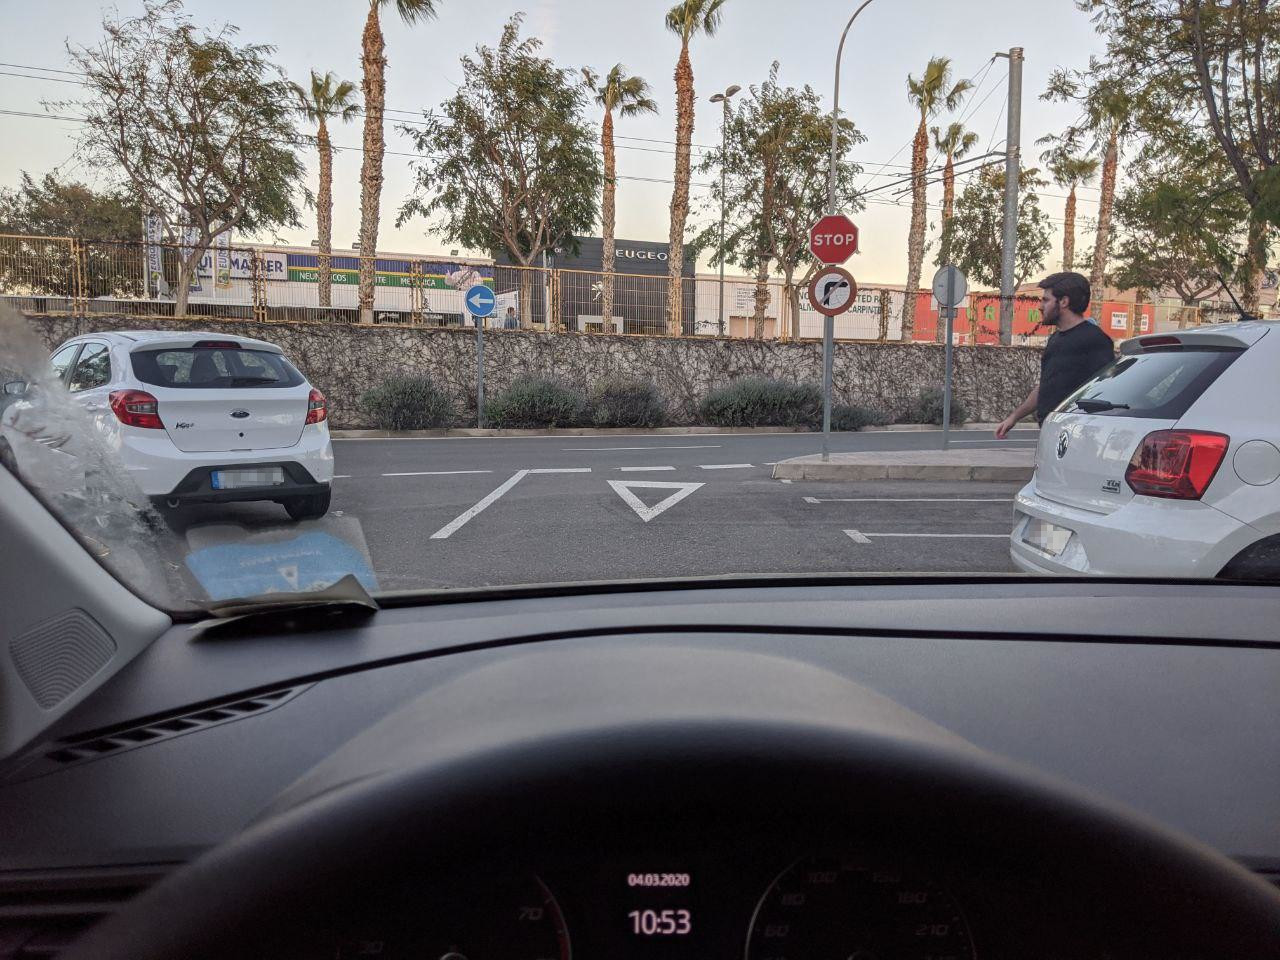
\includegraphics[trim={17cm 7cm 5cm 3cm},clip,width=.25\textwidth]{figures/videoprediction/intro/0.jpg}};
\node[inner sep=0.8pt, draw=blue!70, line width=0.05cm] (frame1) at (0.25,0.25)
    	{\includegraphics[trim={17cm 7cm 5cm 3cm},clip,width=.25\textwidth]{figures/videoprediction/intro/0.jpg}};
\node[inner sep=0.8pt, draw=blue!70, line width=0.05cm] (frame2) at (0.5,0.5)
    	{\includegraphics[trim={17cm 7cm 5cm 3cm},clip,width=.25\textwidth]{figures/videoprediction/intro/0.jpg}};
 \node[inner sep=0.8pt, draw=blue!70, line width=0.05cm] (frame3) at (0.75,0.75)
    	{\includegraphics[trim={17cm 7cm 5cm 3cm},clip,width=.25\textwidth]{figures/videoprediction/intro/0.jpg}};
 \node[inner sep=0.8pt, draw=green!80, line width=0.05cm] (frame4) at (6.5,0.75)
    	{\includegraphics[trim={17cm 7cm 5cm 3cm},clip,width=.25\textwidth]{figures/videoprediction/intro/1_mask.jpg}};
\node[inner sep=0.8pt, draw=green!80, line width=0.05cm] (frame5) at (12.2,0.75)
    	{\includegraphics[trim={17cm 7cm 5cm 3cm},clip,width=.25\textwidth]{figures/videoprediction/intro/2_mask.jpg}};
%\node[inner sep=0.8pt, draw=green!80, line width=0.05cm] (frame5) at (11,0.75)
%    	{\includegraphics[trim={9.5cm 2.8cm 5.5cm 2.5cm},clip,width=.25\textwidth]{figures/introduction/3_mask.jpg}};
\node at (0.4,-3.0) {\LARGE $\mathbf{(X_{t-n}, \ldots, X_{t})}$};
\node at (0.4,3.65) {\LARGE Context Frames};
\node at (6.5,-3.0) {\LARGE $\mathbf{\hat{Y}_{t+1}}$};
\node at (9.5,3.65) {\LARGE Predicted Frames};
\node at (12.2,-3.0) {\LARGE $\mathbf{\hat{Y}_{t+m}}$};
\draw [->,shorten >= 3pt, shorten <= 3pt,line width= 0.5mm] (frame3) -- (frame4);
\path (frame4) -- node[auto=false]{\Huge \ldots} (frame5);
%\draw [->,shorten >= 3pt, shorten <= 3pt,line width= 0.5mm] (frame4) -- (frame5);
%\draw[<->,thick] (russell.south east) -- (whitehead.north west)
%    node[midway,fill=white] {Principia Mathematica};
\end{tikzpicture}}
	\caption{A pedestrian appeared from behind the white car with the intention of crossing the street. The autonomous car must make a call: hit the emergency braking routine or not. This all comes down to predict the next frames~$(\hat{Y}_{t+1},\ldots,\hat{Y}_{t+m})$ given a sequence of context frames~$(X_{t-n}, \ldots, X_{t})$, where $n$ and $m$ denote the number of context and predicted frames, respectively. From these predictions at a representation level (\acs{RGB}, high-level semantics, etc.) a decision-making system would make the car avoid the collision.}
	\label{fig:pedestrian}
\end{figure}

In general terms, the prediction and anticipation of future events is a key component of intelligent decision-making systems. Despite the fact that we, humans, solve this problem quite easily and effortlessly,
%simplicity of the problem from our human perspective, 
it is extremely challenging from a machine's point of view.
%due to the very same complexity of visual appearance and motion. 
Some factors that contribute to such complexity are occlusions, camera movement, lighting conditions, clutter, or object deformations. Even so, video prediction models are able to extract rich spatio-temporal features from natural videos in a self-supervised fashion. This was fostered by the great strides deep learning has made in different research fields such as human action recognition and prediction~\cite{Kong2018}, semantic segmentation~\cite{Garcia2018a}, and registration~\cite{Villena2020}, to name a few. Because of their ability to learn adequate representations from high-dimensional data~\cite{LeCun2015}, deep learning-based models fit perfectly into the learning by prediction paradigm.

\subsection{Application Domains}
Video prediction methods have been successfully applied in a broad range of application domains such as robotics, autonomous driving, action anticipation, and more. Relying on action-conditioned video prediction, robots were able to successfully manipulate previously unseen objects~\cite{Finn2016}. In the same domain, video prediction has facilitated decision making in vision-based robotic control~\cite{Ebert2018} and motion planning~\cite{Koppula2016,Xie2019} and has provided accurate world models, of high-dimensional environments, to model-based~\ac{RL} approaches. For instance, video prediction has enabled planning in unknown environments~\cite{Hafner2019, Kaiser2020}. This has helped model-based~\ac{RL} to achieve similar or better results compared to model-free approaches, with fewer interactions and improved generalization capabilities.

Regarding self-driving cars, the trajectory prediction in traffic of pedestrians~\cite{Bhattacharyya2018} or generic agents~\cite{Choi2020} is extremely useful to anticipate future events. Furthermore, the probabilistic prediction of multi-modal futures~\cite{Hu2020} demonstrated great success when it comes to traffic uncertainty. Likewise, the synergy between video prediction and action anticipation was successfully proven with the prediction of visual embeddings~\cite{Gammulle2019} and motion representations~\cite{Opazo2018}. Some other tasks in which video prediction has been applied successfully are: prediction of instance/semantic segmentation maps~\cite{Luc2018,Bhattacharyya2019,Terwilliger2019}, anomaly detection~\cite{Liu2018a}, precipitation nowcasting~\cite{Shi2015,Shi2017}, and video interpolation~\cite{Liu2017}.

\subsection{Review Scope and Terminology}
In this review, we put our focus on deep learning techniques and how they have been extended or applied to video prediction. We limit this review to the future video prediction given the  context of a sequence of previous frames, leaving aside methods that predict future from a static image. In this context, the terms
%In the context of this review, we refer indistinctively to the prediction of future frames in videos given a sequence of previous frames, through the use of different equivalent expressions such as: 
video prediction, future frame prediction, next video frame prediction, future frame forecasting, and future frame generation are used interchangeably. To the best of our knowledge, this is the first review in the literature that focuses on video prediction using deep learning techniques.


\section{Terminology and Background Concepts}
\label{sec:video_prediction}
Besides its biological roots, video prediction draws inspiration from computational models of the predictive coding paradigm~\cite{Softky1995,Rao1999,Deco2001,Hollingworth2004}. Predictive coding states that human brain builds complex mental representations of the physical and causal rules that govern the world. This arises from the conceptual acquisition and the accumulation of background knowledge from early ages, primarily through observation and interaction~\cite{Cleeremans1991,Cleeremans1993,Baker2014}. From a brain processing perspective, these mental representations are continuously updated through the prediction of raw sensory inputs. The brain refines the already understood world models from the mismatch between its predictions and the actual sensory input~\cite{Ouden2012}.

%Video prediction task closely captures the essence of the predictive coding paradigm and it is considered as the intermediate step between natural videos and decision making. Its potential to extract meaningful representations of the underlying patterns in video data makes the video prediction task a promising avenue for self-supervised representation learning.

\subsection{Problem Definition}
Video prediction closely captures the essence of the predictive coding paradigm. On this basis, video prediction is defined as the task of inferring the subsequent frames in a video, based on a sequence of previous frames used as a context. Let ${\mathbf{X}_{t}\in\mathrm{R}^{w \times h \times c}}$ be the $t$-th frame in the video sequence ${\mathbf{X}=(X_{t-n},\ldots,X_{t-1},X_t)}$ with $n$ frames, where $w$, $h$, and $c$ denote width, height, and number of channels, respectively. The target is to predict the next $m$ frames ${\mathbf{Y}=(\hat{Y}_{t+1},\hat{Y}_{t+2},\ldots,\hat{Y}_{t+m})}$ from the input~$\mathbf{X}$.

Different from video generation that is mostly unconditioned, video prediction is conditioned on a previously learned representation from a sequence of input frames. At a first glance, and in the context of learning paradigms, one can think about the video prediction task as a supervised learning approach because the target frame acts as a label. However, as this information is already available in the input video sequence, no extra labels or human supervision is needed. Therefore, learning by prediction is a self-supervised task, filling the gap between supervised and unsupervised learning. 

Under the assumption that good predictions can only be the result of accurate representations, learning by prediction is a feasible approach to verify how accurately the system has learned the underlying patterns in the input data. In other words, it represents a suitable framework for representation learning~\cite{Bengio2013,Wang2015}. Furthermore, because of its potential to extract meaningful representations from video sequences, video prediction is an excellent intermediate step between natural videos and decision-making.

\subsection{Exploiting the Time Dimension of Videos}
Unlike static images, videos provide complex transformations and motion patterns ordered in the time dimension. Focusing on a small image patch in the same spatial location through consecutive time steps, a wide range of visually similar local deformations are identified due to the temporal coherence. In contrast, when looking at the big picture, the consecutive frames are visually different but semantically coherent. The variability in the visual appearance of a video at different scales, is mainly due to occlusions, changes in the lighting conditions, and camera motion, among other factors. From this source of temporally ordered visual cues, predictive models are able to extract representative spatio-temporal correlations depicting the dynamics in a video sequence. For instance, Agrawal \textit{et al.}~\cite{Agrawal2015} established a direct link between vision and motion, attempting to reduce supervision efforts when training deep predictive models. 

The importance of the time dimension in video understanding models has been well studied~\cite{Huang2018}. The implicit temporal ordering in videos, also known as the arrow of time, indicates whether a video sequence is playing forward or backward. Using this temporal direction as a supervisory signal~\cite{Pickup2014,Misra2016,Wei2018} further encouraged predictive models to implicitly or explicitly model spatio-temporal correlations of a video sequence to understand the dynamics of a scene. The time dimension of a video reduces the supervision effort and makes the prediction task self-supervised.

\subsection{Dealing with Stochasticity}
\begin{figure}
	\centering
	\resizebox{0.8\textwidth}{!}{
		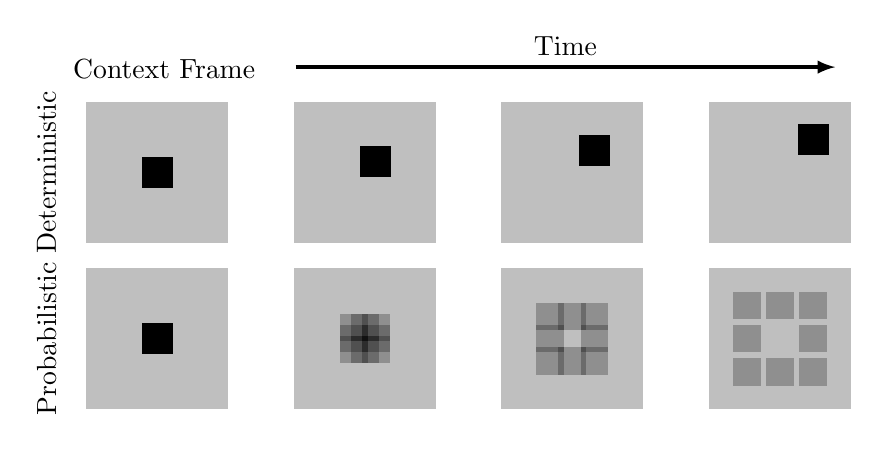
\begin{tikzpicture}[]
	\tikzset{box/.style={black, draw=black, fill=none, very thick, minimum height=4 em, minimum width=16 em}}

	\foreach \k in {0,...,3}
	{
		\foreach \i in {0,...,4}
		{
			\foreach \j in {0,...,4}
			{
				\node[box, fill=gray!50, draw=gray!50, minimum height=1 em, minimum width=1 em] (l1-\i-\j-\k) at (\i em + 0.75 em * \k em, \j em) {};
			}
		}
	}

	\node[box, fill=black, draw=black, minimum height=1 em, minimum width=1 em] at (l1-2-2-0){};
	%\node[box, fill=black, draw=black, minimum height=1 em, minimum width=1 em] at ([yshift=0.25em, xshift=0.25em]l1-2-2-1){};
	%\node[box, fill=black, draw=black, minimum height=1 em, minimum width=1 em] at ([yshift=0.4em, xshift=0.4em]l1-2-2-2){};
	%\node[box, fill=black, draw=black, minimum height=1 em, minimum width=1 em] at ([yshift=0.6em, xshift=0.6em]l1-2-2-3){};
	
	\node[box, fill=black, draw=black, minimum height=1 em, minimum width=1 em] at ([yshift=0.4em, xshift=0.4em]l1-2-2-1){};
	\node[box, fill=black, draw=black, minimum height=1 em, minimum width=1 em] at ([yshift=0.8em, xshift=0.8em]l1-2-2-2){};
	\node[box, fill=black, draw=black, minimum height=1 em, minimum width=1 em] at ([yshift=1.2em, xshift=1.2em]l1-2-2-3){};

	\foreach \k in {0,...,3}
	{
		\foreach \i in {0,...,4}
		{
			\foreach \j in {0,...,4}
			{
				\node[box, fill=gray!50, draw=gray!50, minimum height=1 em, minimum width=1 em] (l2-\i-\j-\k) at (\i em + 0.75 em * \k em, \j em - 6 em) {};
			}
		}
	}

	\node[box, fill=black, draw=black, minimum height=1 em, minimum width=1 em] at (l2-2-2-0){};

	%\node[box, fill=black, draw=black, minimum height=1 em, minimum width=1 em] at ([yshift=0.25em, xshift=0.25em]l1-2-2-1){};

	%\node[box, fill=black, draw=black, minimum height=1 em, minimum width=1 em] at ([yshift=0.4em, xshift=0.4em]l1-2-2-2){};

	\node[box, fill=black, draw=none, minimum height=1 em, minimum width=1 em, opacity=0.25] at ([yshift=-0.4em, xshift=0em]l2-2-2-1){};
	\node[box, fill=black, draw=none, minimum height=1 em, minimum width=1 em, opacity=0.25] at ([yshift=0.4em, xshift=0em]l2-2-2-1){};
	\node[box, fill=black, draw=none, minimum height=1 em, minimum width=1 em, opacity=0.25] at ([yshift=-0.4em, xshift=0.4em]l2-2-2-1){};
	\node[box, fill=black, draw=none, minimum height=1 em, minimum width=1 em, opacity=0.25] at ([yshift=0em, xshift=0.4em]l2-2-2-1){};
	\node[box, fill=black, draw=none, minimum height=1 em, minimum width=1 em, opacity=0.25] at ([yshift=0.4em, xshift=0.4em]l2-2-2-1){};
	\node[box, fill=black, draw=none, minimum height=1 em, minimum width=1 em, opacity=0.25] at ([yshift=-0.4em, xshift=-0.4em]l2-2-2-1){};
	\node[box, fill=black, draw=none, minimum height=1 em, minimum width=1 em, opacity=0.25] at ([yshift=0em, xshift=-0.4em]l2-2-2-1){};
	\node[box, fill=black, draw=none, minimum height=1 em, minimum width=1 em, opacity=0.25] at ([yshift=0.4em, xshift=-0.4em]l2-2-2-1){};

	\node[box, fill=black, draw=none, minimum height=1 em, minimum width=1 em, opacity=0.25] at ([yshift=-0.8em, xshift=0em]l2-2-2-2){};
	\node[box, fill=black, draw=none, minimum height=1 em, minimum width=1 em, opacity=0.25] at ([yshift=0.8em, xshift=0em]l2-2-2-2){};
	\node[box, fill=black, draw=none, minimum height=1 em, minimum width=1 em, opacity=0.25] at ([yshift=-0.8em, xshift=0.8em]l2-2-2-2){};
	\node[box, fill=black, draw=none, minimum height=1 em, minimum width=1 em, opacity=0.25] at ([yshift=0em, xshift=0.8em]l2-2-2-2){};
	\node[box, fill=black, draw=none, minimum height=1 em, minimum width=1 em, opacity=0.25] at ([yshift=0.8em, xshift=0.8em]l2-2-2-2){};
	\node[box, fill=black, draw=none, minimum height=1 em, minimum width=1 em, opacity=0.25] at ([yshift=-0.8em, xshift=-0.8em]l2-2-2-2){};
	\node[box, fill=black, draw=none, minimum height=1 em, minimum width=1 em, opacity=0.25] at ([yshift=0em, xshift=-0.8em]l2-2-2-2){};
	\node[box, fill=black, draw=none, minimum height=1 em, minimum width=1 em, opacity=0.25] at ([yshift=0.8em, xshift=-0.8em]l2-2-2-2){};

	\node[box, fill=black, draw=none, minimum height=1 em, minimum width=1 em, opacity=0.25] at ([yshift=-1.2em, xshift=0em]l2-2-2-3){};
	\node[box, fill=black, draw=none, minimum height=1 em, minimum width=1 em, opacity=0.25] at ([yshift=1.2em, xshift=0em]l2-2-2-3){};
	\node[box, fill=black, draw=none, minimum height=1 em, minimum width=1 em, opacity=0.25] at ([yshift=-1.2em, xshift=1.2em]l2-2-2-3){};
	\node[box, fill=black, draw=none, minimum height=1 em, minimum width=1 em, opacity=0.25] at ([yshift=0em, xshift=1.2em]l2-2-2-3){};
	\node[box, fill=black, draw=none, minimum height=1 em, minimum width=1 em, opacity=0.25] at ([yshift=1.2em, xshift=1.2em]l2-2-2-3){};
	\node[box, fill=black, draw=none, minimum height=1 em, minimum width=1 em, opacity=0.25] at ([yshift=-1.2em, xshift=-1.2em]l2-2-2-3){};
	\node[box, fill=black, draw=none, minimum height=1 em, minimum width=1 em, opacity=0.25] at ([yshift=0em, xshift=-1.2em]l2-2-2-3){};
	\node[box, fill=black, draw=none, minimum height=1 em, minimum width=1 em, opacity=0.25] at ([yshift=1.2em, xshift=-1.2em]l2-2-2-3){};

	\node at ([yshift=1.75 em, xshift=-1.75 em]l1-4-4-0) { Context Frame};
	\draw[-latex, very thick] ([yshift=1.25 em, xshift=3 em]l1-4-4-0.north) -- node [yshift=0.75 em]{Time}([yshift=1.25 em]l1-4-4-3.north);

	\node[rotate=90] at ([yshift=-2 em, xshift=-6 em]l1-4-4-0.center) {Deterministic};
	\node[rotate=90] at ([yshift=-2 em, xshift=-6 em]l2-4-4-0.center) {Probabilistic};

\end{tikzpicture}
	}
	\caption{At top, a deterministic environment where a geometric object, e.g. a black square, starts moving following a random direction. At bottom, probabilistic outcome. Darker areas correspond to higher probability outcomes. As uncertainty is introduced, probabilities get blurry and averaged. Figure inspired by~\cite{Babaeizadeh2018}.}
	\label{fig:deterministic}
\end{figure}
Predicting how a square is moving, could be extremely challenging even in a deterministic environment such as the one represented in Figure~\ref{fig:deterministic}. The lack of contextual information and the multiple equally probable outcomes hinder the prediction task. But, what if we use two consecutive frames as context? Under this configuration and assuming a physically perfect environment, the square will be indefinitely moving in the same direction. This represents a deterministic outcome, an assumption that many authors made in order to deal with future uncertainty. Assuming a deterministic outcome would narrow the prediction space to a unique solution. However, this assumption is not suitable for natural videos. The future is by nature multimodal, 
%%%(done) AAA: What is the meaning of "multimodal future"?
since the probability distribution defining all the possible future outcomes in a context has multiple modes, i.e. there are multiple equally probable and valid outcomes. Furthermore, on the basis of a deterministic universe, we indirectly assume that all possible outcomes are reflected in the input data. These assumptions make the prediction under uncertainty an extremely challenging task. 

Most of the existing deep learning-based models in the literature are deterministic. Although the future is uncertain, a deterministic prediction would suffice some easily predictable situations. For instance, most of the movement of a car is largely deterministic, while only a small part is uncertain. However, when multiple predictions are equally probable, a deterministic model will learn to average between all the possible outcomes. This averaging effect depends on the loss function and is visually represented in predictions as blurriness, specially on long time horizons. However, it can be mitigated by constructing a loss function that does not lead to averaging. As deterministic models are unable to handle real-world settings characterized by chaotic dynamics, authors considered that incorporating uncertainty to the model is a crucial aspect. Probabilistic approaches dealing with these issues are discussed in Section~\ref{subsec:m_uncertainty}.

\subsection{The Devil is in the Loss Function}
The design and selection of the loss function for the video prediction task is of utmost importance. Pixel-wise losses, e.g. $\ell_2$, $\ell_1$ and \ac{MSE}, are widely used in both unstructured and structured predictions. Although leading to plausible predictions in deterministic scenarios, such as synthetic datasets and video games, they struggle with the inherent uncertainty of natural videos. In a probabilistic environment, with different equally probable outcomes, pixel-wise losses aim to accommodate uncertainty by blurring the prediction, as we can observe in Figure \ref{fig:deterministic}. In other words, the deterministic loss functions average out multiple equally plausible outcomes in a single, blurred prediction. In the pixel space, these losses are unstable to slight deformations and fail to capture discriminative representations to efficiently regress the broad range of possible outcomes. This makes difficult to draw predictions maintaining the consistency with our visual similarity notion. A recent study~\cite{Aigner2020} performed an in-depth analysis of the generalization capabilities of different loss functions for the video prediction task. Besides video prediciton, the impact of different loss functions was analyzed in image restoration restoration~\cite{Zhao2017}, classification~\cite{Janocha2017}, camera pose regression~\cite{Kendall2017} and structured prediction~\cite{Hwang2019}, among others. This fosters reasoning about the importance of the loss function, particularly when making long-term predictions in high-dimensional and multimodal natural videos.

%\textbf{Pixel-wise losses}. 
Most of distance-based loss functions, such as based on $\ell_p$ norm, come from the assumption that data is drawn from a Gaussian distribution. But, how these loss functions address multimodal distributions? Assuming that a pixel is drawn from a bimodal distribution with two equally likely modes $Mo_1$ and $Mo_2$, the mean value ${\overline{Mo}=(Mo_1 + Mo_2)/2}$ would minimize the $\ell_p$-based losses over the data, even if $\overline{Mo}$ has very low probability~\cite{Mathieu2016}. This suggests that the average of two equally probable outcomes would minimize distance-based losses such as, the \ac{MSE} loss. However, this applies to a lesser extent when using $\ell_1$ norm as the pixel values would be the median of the two equally likely modes in the distribution. In contrast to the $\ell_2$ norm that emphasizes outliers with the squaring term, the $\ell_1$ promotes sparsity thus making it more suitable for prediction in high-dimensional data \cite{Mathieu2016}. Based on the $\ell_2$ norm, the \ac{MSE} is also commonly used in the training of video prediction models. However, it produces low reconstruction errors by merely averaging all the possible outcomes in a blurry prediction as uncertainty is introduced. In other words, the mean image would minimize the \ac{MSE} error as it is the global optimum, thus avoiding finer details such as facial features and subtle movements as they are noise for the model. Most of the video prediction approaches rely on pixel-wise loss functions, obtaining roughly accurate predictions in easily predictable datasets.

%%%(done) AAA: The remainder of this section is a long, difficult to read itemized list of approaches. It should be described as a collection of different strategies not in itemized form but rather as a running text. 
One of the ultimate goals of many video prediction approaches is to palliate the blurry predictions when it comes to uncertainty. For this purpose, authors broadly focused on: directly improving the loss functions; exploring adversarial training; alleviating the training process by reformulating the problem in a higher-level space; or exploring probabilistic alternatives. Some promising results were reported by combining the loss functions with sophisticated regularization terms, e.g. the \ac{GDL} to enhance prediction sharpness~\cite{Mathieu2016} and the \ac{TV} regularization to reduce visual artifacts and enforce coherence~\cite{Liu2017}. Perceptual losses were also used to further improve the visual quality of the predictions~\cite{Dosovitskiy2016,Johnson2016,Ledig2017,Sajjadi2017,Zhu2016}. However, in light of the success of the \acp{GAN}, adversarial training emerged as a promising alternative to disambiguate between multiple equally probable modes. It was widely used in conjunction with different distance-based losses such as: \ac{MSE}~\cite{Lotter2015}, $\ell_2$~\cite{Chen2017,Jin2017,Wichers2018}, or a combination of them~\cite{Mathieu2016,Villegas2017,Walker2017,Liang2017,Luc2017,Hu2019}. To alleviate the training process, many authors reformulated the optimization process in a higher-level space (see Section \ref{subsec:m_high_level}). While great strides have been made to mitigate blurriness, most of the existing approaches still rely on distance-based loss functions. As a consequence, the regress-to-the-mean problem remains an open issue. This has further encouraged authors to reformulate existing deterministic models in a probabilistic fashion.
%To palliate the blurry predictions when dealing with uncertainty, the authors: (1) combined distance-based loss functions with sophisticated regularization terms, such as the \gls{gdl} to enhance prediction sharpness by focusing on image gradients~\cite{Mathieu2016}, and adding spatio-temporal regularization to the $\ell_1$ loss~\cite{Liu2017}; (2) uses adversarial training to disambiguate between modes alongside, \gls{mse}~\cite{Lotter2015}, $\ell_2$~\cite{Chen2017,Jin2017,Wichers2018}, a combination of losses~\cite{Mathieu2016,Villegas2017,Walker2017,Liang2017,Luc2017,Hu2019}; (3) reformulate the optimization in a higher-level space. Although the training process becomes easier, we still have to deal with the regress-to-the-mean issue; (4) uses perceptual losses to further improve the visual quality of the predictions~\cite{Dosovitskiy2016,Johnson2016,Ledig2017,Sajjadi2017,Zhu2016}; and (5) extends existing deterministic models with latent variables to model uncertainty, or directly sample different outcomes from a posterior distribution modeled with a probabilistic approach. The latter is extensively addressed in Section~\ref{subsec:m_uncertainty}.

\section{Backbone Deep Learning Architectures}
\label{cha:videoprediction:sec:background}
In this section, we will briefly review the most common deep networks that are used as building blocks for the video prediction models discussed in this review: convolutional neural networks, recurrent networks, and generative models.

\subsection{Convolutional Models}
Convolutional layers are the basic building blocks of deep learning architectures designed for visual reasoning since the \acp{CNN} efficiently model the spatial structure of images~\cite{Lecun1998}. As we focus on the visual prediction, \acp{CNN} represent the foundation of predictive learning literature. However, their performance is limited by the intra-frame and inter-frame dependencies.

Convolutional operations account for short-range intra-frame dependencies due to their limited receptive fields, determined by the kernel size. This is a well-addressed issue, that many authors circumvented by (1) stacking more convolutional layers~\cite{Jain2007}, (2) increasing the kernel size (although it becomes prohibitively expensive), (3) by linearly combining multiple scales~\cite{Mathieu2016} as in the reconstruction process of a Laplacian pyramid~\cite{Denton2015}, (4) using dilated convolutions to capture long-range spatial dependencies~\cite{Yu2017}, (5) enlarging the receptive fields~\cite{Chen2018, Luo2016}, or subsampling, i.e. using pooling operations in exchange for losing resolution. The latter could be mitigated by using residual connections~\cite{He2016,Villegas2017a} to preserve resolution while increasing the number of stacking convolutions. But even addressing these limitations, would \acp{CNN} be able to predict in a longer time horizon?
%%%(done) AAA: Note that in the problem definition section, the problem is defined as predicting the $t+1$ frame given the first $t$ frames. Thus, the "longer time horizon" is outside the scope of the problem definition... 

Vanilla~\acp{CNN} lack of explicit inter-frame modeling capabilities. To properly model inter-frame variability in a video sequence, 3D convolutions come into play as a promising alternative to recurrent modeling. Several video prediction approaches leveraged 3D convolutions to capture temporal consistency~\cite{Wang2019b,Vondrick2016,Tulyakov2018,Aigner2018,Zhang2019}. Also modeling time dimension, Amersfoort \textit{et al.} \cite{Amersfoort2017} replicated a purely convolutional approach in time to address multi-scale predictions in the transformation space. In this case, the learned affine transforms at each time step play the role of a recurrent state.

\subsection{Recurrent Models}
Recurrent models were specifically designed to model a spatio-temporal representation of sequential data such as video sequences. Among other sequence learning tasks, such as machine translation, speech recognition and video captioning, to name a few, \acp{RNN}~\cite{Rumelhart1986} demonstrated great success in the video prediction scenario~\cite{Ranzato2014,Srivastava2015,Shi2015,Lotter2017,Lotter2015,Byeon2018, Zhang2019,Patraucean2015,Lu2017,Villegas2017,Denton2017,Chen2017,Oh2015,Denton2018,Villegas2017,Nabavi2018,Vora2018,Sun2019,Terwilliger2019,Wichers2018,Minderer2019}. Vanilla \acp{RNN} have some important limitations when dealing with long-term representations due to the vanishing and exploding gradient issues, making the \ac{BPTT} cumbersome. By extending classical \acp{RNN} to more sophisticated recurrent models, such as \ac{LSTM}~\cite{Hochreiter1997} and \ac{GRU}~\cite{Cho2014}, these problems were mitigated. Shi \textit{et al.} extended the use of \ac{LSTM}-based models to the image space~\cite{Shi2015}. While some authors explored \ac{MDLSTM}~\cite{Graves2007}, others stacked recurrent layers to capture abstract spatio-temporal correlations~\cite{Lotter2015,Finn2016}. Zhang \textit{et al.} addressed the duplicated representations along the same recurrent paths~\cite{Zhan2019}.

\subsection{Generative Models}
Whilst discriminative models learn the decision boundaries between classes, generative models learn the underlying distribution of individual classes. More formally, discriminative models capture the conditional probability $p(y|x)$, while generative models capture the joint probability $p(x,y)$, or $p(x)$ in the absence of labels $y$. The goal of generative models is the following: given some training data, generate new samples from the same distribution. Let input data~$\sim p_{data}(x)$ and generated samples~$\sim p_{model}(x)$ where, $p_{data}$ and $p_{model}$ are the underlying input data and model's probability distribution respectively. The training process consists in learning a $p_{model}(x)$ similar to $p_{data}(x)$. This is done by explicitly, e.g \acp{VAE}, or implicitly, e.g. \acp{GAN}, estimating a density function from the input data. In the context of video prediction, generative models are mainly used to cope with future uncertainty by generating a wide spectrum of feasible predictions rather than a single eventual outcome.

\subsubsection{Explicit Density Modeling}
These models explicitly define and solve for $p_{model}(x)$. 

\vspace*{0.1cm}\noindent\textbf{PixelRNNs and PixelCNNs~\cite{Oord2016}}: These are a type of \acp{FVBN}~\cite{Neal1992,Bengio1999} that explicitly define a tractable density and estimate the joint distribution $p(x)$ as a product of conditional distributions over the pixels. Informally, they turn pixel generation into a sequential modeling problem, where next pixel values are determined by previously generated ones. In PixelRNNs, this conditional dependency on previous pixels is modeled using \ac{2D} \acp{LSTM}. On the other hand, dependencies are modeled using convolutional operations over a context region, thus making training faster. In a nutshell, these methods are outputting a distribution over pixel values at each location in the image, aiming to maximize the likelihood of the training data being generated. Further improvements of the original architectures have been carried out to address different issues. The Gated PixelCNN~\cite{Oord2016a} is computationally more efficient and improves the receptive fields of the original architecture. In the same work, authors also explored conditional modeling of natural images, where the joint probability distribution is conditioned on a latent vector ---it represents a high-level image description. This further enabled the extension to video prediction~\cite{Kalchbrenner2016}. 

\vspace*{0.1cm}\noindent\textbf{\acp{VAE}}: These models are an extension of \acp{AE} that encode and reconstruct its own input data $x$ in order to capture a low-dimensional representation $z$ containing the most meaningful factors of variation in $x$. Extending this architecture to generation, \acp{VAE} aim to sample new images from a prior over the underlying latent representation $z$. \acp{VAE} represent a probabilistic spin over the deterministic latent space in \acp{AE}. Instead of directly optimizing the density function, which is intractable, they derive and optimize a lower bound on the likelihood. Data is generated from the learned distribution by perturbing the latent variables. In the video prediction context, \acp{VAE} are the foundation of many probabilistic models dealing with future uncertainty~\cite{Liang2017,Babaeizadeh2018,Denton2018,Fragkiadaki2017,Castrejon2019,Bhattacharyya2019,Minderer2019}. Although these variational approaches are able to generate various plausible outcomes, the predictions are blurrier and of lower quality compared to state-of-the-art \ac{GAN}-based models. Many approaches were taken to leverage the advantages of variational inference: combined adversarial training with \acp{VAE}~\cite{Liang2017}, and others incorporated latent probabilistic variables into deterministic models, such as \acp{VRNN}~\cite{Chung2015,Castrejon2019} and \acp{VED}~\cite{Henaff2017}.

\subsubsection{Implicit Density Modeling}
These models learn to sample from $p_{model}$ without explicitly defining it. 

\vspace*{0.1cm}\noindent\textbf{\acp{GAN}}~\cite{Goodfellow2014}: are the backbone of many video prediction approaches~\cite{Mathieu2016,Lotter2015,Liang2017,Hu2019,Chen2017,Wichers2018,Jin2017,Walker2017,Villegas2017,Kwon2019,Vondrick2017, Villegas2017a,Lu2017,Zhou2016,Bhattacharjee2017,Vondrick2016,Saito2017,Chen2017a,Tulyakov2018}. Inspired on game theory, these networks consist of two models that are jointly trained as a minimax game to generate new fake samples that resemble the real data. On one hand, we have the discriminator model featuring a probability distribution function describing the real data. On the other hand, we have the generator which tries to generate new samples that fool the discriminator. In their original formulation, \acp{GAN} are unconditioned --the generator samples new data from a random noise, e.g. Gaussian noise. Nevertheless, Mirza \textit{et al.}~\cite{Mirza2014} proposed the \ac{CGAN}, a conditional version where the generator and discriminator are conditioned on some extra information, e.g. class labels, previous predictions, and multimodal data, among others. \acp{CGAN} are suitable for video prediction, since the spatio-temporal coherence between the generated frames and the input sequence is guaranteed. The use of adversarial training for the video prediction task, represented a leap over the previous state-of-the-art methods in terms of prediction quality and sharpness. However, adversarial training is unstable. Without an explicit latent variable interpretation, \acp{GAN} are prone to mode collapse ---generator fails to cover the space of possible predictions by getting stuck into a single mode~\cite{Henaff2017,Lee2018}. Moreover, \acp{GAN} often struggle to balance between the adversarial and reconstruction loss, thus getting blurry predictions. Among the dense literature on adversarial networks, we find some other interesting works addressing \acp{GAN} limitations~\cite{Radford2016,Arjovsky2017}.

\section{Datasets}
\label{sec:datasets}
As video prediction models are mostly self-supervised, they need video sequences as input data. However, some video prediction methods rely on extra supervisory signals, e.g. segmentation maps, and human poses. This makes out-of-domain video datasets perfectly suitable for video prediction. This section describes the most relevant datasets, discussing their pros and cons. Datasets were organized according to their main purpose and summarized in Table~\ref{table:datasets}.

\subsection{Action and Human Pose Recognition Datasets}
\vspace*{0.1cm}\noindent\textbf{KTH~\cite{Schuldt2004}}: is an action recognition dataset which includes \num{2391} video sequences of \num{4} seconds mean duration, each of them containing an actor performing an action taken with a static camera, over homogeneous backgrounds, at \num{25} \ac{FPS} and with its resolution downsampled to $160 \times 120$ pixels. Just \num{6} different actions are performed, but it was the biggest dataset of this kind at its moment.

\vspace*{0.1cm}\noindent\textbf{Weizmann~\cite{Gorelick2007}}: is also an action recognition dataset, created for modelling actions as space-time shapes. For this reason, it was recorded at a higher frame rate (\num{50} \ac{FPS}). It just includes \num{90} video sequences, but performing 10 different actions. It uses a static-camera, homogeneous backgrounds and low resolution ($180 \times 144$ pixels). KTH and Weizmann are usually used together due to their similarities in order to augment the amount of available data.

\vspace*{0.1cm}\noindent\textbf{HMDB-51~\cite{Kuehne2011}}: is a large-scale database for human motion recognition. It claims to represent the richness of human motion taking profit from the huge amount of video available online. It is composed by \num{6766} normalized videos (with mean duration of \num{3.15} seconds) where humans appear performing one of the 51 considered action categories. Moreover, a stabilized dataset version is provided, in which camera movement is disabled by detecting static backgrounds and displacing the action as a window. It also provides interesting data for each sequence such as body parts visible, point of view respect the human, and if there is camera movement or not. It also exists a joint-annotated version called J-HMBD~\cite{Jhuang2013} in which the key points of joints were mannually added for 21 of the HMDB actions.

\vspace*{0.1cm}\noindent\textbf{UCF101~\cite{Soomro2012}}: is an action recognition dataset of realistic action videos, collected from YouTube. It has 101 different action categories, and it is an extension of UCF50, which has \num{50} action categories. All videos have a frame rate of 25 \ac{FPS} and a resolution of $320 \times 240$ pixels. Despite being the most used dataset among predictive models, a problem it has is that only a few sequences really represent movement, i.e. they often show an action over a fixed background.

\vspace*{0.1cm}\noindent\textbf{Penn Action Dataset~\cite{Zhang2013}}: is an action and human pose recognition dataset from the University of Pennsylvania. It contains \num{2326} video sequences of \num{15} different actions, and it also provides human joint and viewpoint (position of the camera respect the human) annotations for each sequence. Each action is balanced in terms of different viewpoints representation.

\vspace*{0.1cm}\noindent\textbf{Human3.6M~\cite{Ionescu2014}}: is a human pose dataset in which \num{11} actors with marker-based suits were recorded performing \num{15} different types of actions. It features RGB images, depth maps (time-of-flight range data), poses and scanned 3D surface meshes of all actors. Silhouette masks and 2D bounding boxes are also provided. Moreover, the dataset was extended by inserting high-quality 3D rigged human models (animated with the previously recorded actions) in real videos, to create a realistic and complex background.

\vspace*{0.1cm}\noindent\textbf{THUMOS-15~\cite{Idrees2017}}: is an action recognition challenge that was celebrated in 2015. It didn't just focus on recognizing an action in a video, but also on determining the time span in which that action occurs. With that purpose, the challenge provided a dataset that extends UCF101~\cite{Soomro2012} (trimmed videos with one action) with 2100 untrimmed videos where one or more actions take place (with the correspondent temporal annotations) and almost \num{3000} relevant videos without any of the \num{101} proposed actions.

\subsection{Driving and Urban Scene Understanding Datasets}
\textbf{CamVid~\cite{Brostow2008}}: the Cambridge-driving Labeled Video Database is a driving/urban scene understanding dataset which consists of \num{5} video sequences recorded with a $960 \times 720$ pixels resolution camera mounted on the dashboard of a car. Four of those sequences were sampled at \num{1} \ac{FPS}, and one at \num{15} \ac{FPS}, resulting in \num{701} frames which were manually per-pixel annotated for semantic segmentation (under \num{32} classes). It was the first video sequence dataset of this kind to incorporate semantic annotations.

\vspace*{0.1cm}\noindent\textbf{CalTech Pedestrian Dataset~\cite{Dollar2009}}: is a driving dataset focused on detecting pedestrians, since its unique annotations are pedestrian bounding boxes. It is conformed of approximately \num{10} hours of $640 \times 480$ $30$\ac{FPS} video taken from a vehicle driving through regular traffic in an urban environment, making a total

\begin{landscape}
	\ra{1.1}
	\scriptsize
		\begin{ThreePartTable}
			\begin{TableNotes}[normal,flushleft]
				\scriptsize
				\item[1] some dataset names have been abbreviated to enhance table's readability.
				\item[2] values estimated based on the framerate and the total number of frames or videos, as the original values are not provided by the authors.
				\item[3] \textit{custom} indicates that as many frames as needed can be generated. This is related to datasets generated from a game, algorithm or simulation, involving interaction or randomness.
			\end{TableNotes}
			\setlength\LTleft{0pt}
			\setlength\LTright{0pt}
			\begin{longtable}[t]{@{\extracolsep{\fill}}lcccccccccccccc@{}}
				\caption{Summary of the most widely used datasets for video prediction (\textbf{S/R}:~\textbf{S}ynthetic/\textbf{R}eal, \textbf{st}:~\textbf{st}ereo, \textbf{de}:~\textbf{de}pth,
					\textbf{ss}:~\textbf{s}emantic \textbf{s}egmentation, \textbf{is}:~\textbf{i}nstance \textbf{s}egmentation, \textbf{sem}:~\textbf{sem}antic, \textbf{I/O}:~\textbf{I}ndoor/\textbf{O}utdoor environment, \textbf{bb}:~\textbf{b}ounding \textbf{b}ox, \textbf{Act}:~\textbf{Act}ion label, \textbf{ann}:~\textbf{ann}otated, \textbf{env}:~\textbf{env}ironment, \textbf{ToF}:~\textbf{T}ime \textbf{o}f \textbf{F}light, \textbf{vp}:~camera \textbf{v}iew\textbf{p}oints respect human).} \\
				\toprule
				& & & & & & & & \multicolumn{6}{c}{\textbf{provided data and ground-truth}} & \\
				\cmidrule(lr){9-14}
				\textbf{name}\tnote{1} & \textbf{year} & \textbf{S/R} & \textbf{\#videos} & \textbf{\#frames} & \textbf{\#ann. frames} & \textbf{resolution} & \textbf{\#classes} & \textbf{RGB} & \textbf{st} & \textbf{de} & \textbf{ss} & \textbf{is} & \textbf{other annotations} & \textbf{env.}\\
				\midrule
				\endhead
				\insertTableNotes
				\endfoot
				\multicolumn{15}{c}{\textbf{Action and human pose recognition datasets}} \\
				\midrule
				KTH \cite{Schuldt2004} & \num{2004} & R & \num{2391} & \num{250000}\tnote{2} & \num{0} & $160 \times 120$ & \num{6} (action) & \checkmark & \xmark & \xmark & \xmark & \xmark & Act. & O \\
				Weizmann \cite{Gorelick2007} & \num{2007} & R & \num{90} & \num{9000}\tnote{2} & \num{0} & $180 \times 144$ & \num{10} (action) & \checkmark & \xmark & \xmark & \xmark & \xmark & Act. & O  \\
				HMDB-51 \cite{Kuehne2011} & \num{2011} & R & \num{6766} & \num{639300} & \num{0} & $var~\times 240$ & \num{51} (action) & \checkmark & \xmark & \xmark & \xmark & \xmark & Act., vp & I/O\\
				UCF101 \cite{Soomro2012} & \num{2012} & R & \num{13320} & \num{2000000}\tnote{2} & \num{0} & $320 \times 240$ & \num{101} (action) & \checkmark & \xmark & \xmark & \xmark & \xmark & Act. & I/O \\
				Penn Action D. \cite{Zhang2013} & \num{2013} & R & \num{2326} & \num{163841} & \num{0} & $480 \times 270$ & \num{15} (action) & \checkmark & \xmark & \xmark & \xmark & \xmark & Act., Human poses, vp & I/O \\
				Human3.6M \cite{Ionescu2014} & \num{2014} & SR & \num{4000}\tnote{2} & \num{3600000} & \num{0} & $1000 x 1000$ & \num{15} (action) & \checkmark & \xmark & ToF & \xmark & \xmark & Act., Human poses \& meshes & I/O  \\
				THUMOS-15 \cite{Idrees2017} & \num{2017} & R & \num{18404} & \num{3000000}\tnote{2} & \num{0} & $320 \times 240$ & \num{101} (action) & \checkmark & \xmark & \xmark & \xmark & \xmark & Act., Time span & I/O \\
				\midrule
				\multicolumn{15}{c}{\textbf{Driving and urban scene understanding datasets}} \\
				\midrule
				Camvid \cite{Patraucean2015} & \num{2008} & R & \num{5} & \num{18202} & \num{701} (ss) & $960 \times 720$ & \num{32} (sem) & \checkmark & \xmark & \xmark & \checkmark & \xmark & \xmark & O \\
				CalTech Pedest. \cite{Dollar2009} & \num{2009} & R & \num{137} & \num{1000000}\tnote{2} & \num{250000} (bb) & $640 \times 480$ & - & \checkmark & \xmark & \xmark & \xmark & \xmark & Pedestrian bb \& occlusions & O \\
				Kitti \cite{Geiger2013} & \num{2013} & R & \num{151} & \num{48791} & \num{200} (ss) & $1392 \times 512$ & \num{30} (sem) & \checkmark & \checkmark & LiDAR & \checkmark & \checkmark & Odometry & O  \\
				Cityscapes \cite{Cordts2016} & \num{2016} & R & \num{50} & \num{7000000}\tnote{2} & \num{25000} (ss) & $2048 \times 1024$ & \num{30} (sem) & \checkmark & \checkmark & stereo & \checkmark & \checkmark & Odometry, temp, GPS & O \\
				Comma.ai \cite{Lotter2017} & \num{2016} & R & \num{11} & \num{522000}\tnote{2} & \num{0} & $160 \times 320$ & - & \checkmark & \xmark & \xmark & \xmark & \xmark & Steering angles \& speed & O \\
				Apolloscape \cite{Huang2018a} & \num{2018} & R & \num{4} & \num{200000} & \num{146997} (ss) & $3384 \times 2710$ & \num{25} (sem) & \checkmark & \checkmark & LiDAR & \checkmark & \checkmark & Odometry, GPS & O \\	
				\midrule
				\multicolumn{15}{c}{\textbf{Object and video classification datasets}} \\
				\midrule
				Sports1m \cite{Karpathy2014} & \num{2014} & R & \num{1133158} & n/a & \num{0} & $640 \times 360$ $(var.)$ & \num{487} (sport) & \checkmark & \xmark & \xmark & \xmark & \xmark & Sport label & I/O \\
				YouTube8M \cite{Abu-El-Haija2016} & \num{2016} & R & \num{8200000} & n/a & \num{0} & $variable$ & \num{1000} (topic) & \checkmark & \xmark & \xmark & \xmark & \xmark & Topic label, Segment info & I/O \\	
				YFCC100M \cite{Thomee2016} & \num{2016} & SR & \num{8000} & n/a & \num{0} & $variable$ & - & \checkmark & \xmark & \xmark & \xmark & \xmark  & User tags, Localization & I/O \\
				\midrule
				\multicolumn{15}{c}{\textbf{Video prediction datasets}} \\
				\midrule
				Bouncing balls \cite{Sutskever2008} & \num{2008} & S & \num{4000} & \num{20000} & \num{0} & $150 \times 150$ & - & \checkmark & \xmark & \xmark & \xmark & \xmark & \xmark & - \\
				Van Hateren \cite{Cadieu2012} & \num{2012} & R & \num{56} & \num{3584} & \num{0} & $128 \times 128$ & - & \checkmark & \xmark & \xmark & \xmark & \xmark & \xmark & I/O \\
				NORBvideos \cite{Memisevic2013} & \num{2013} & R & \num{110560} & \num{552800} & All (is) & $640 \times 480$ & \num{5} (object) & \checkmark & \xmark & \xmark & \xmark & \checkmark & \xmark & I \\
				Moving MNIST \cite{Srivastava2015} & \num{2015} & SR & $custom$\tnote{3} & $custom$\tnote{3} & \num{0} & $64 \times 64$ & - & \checkmark & \xmark & \xmark & \xmark & \xmark & \xmark & - \\
				Robotic Pushing \cite{Finn2016} & \num{2016} & R & \num{57000} & \num{1500000}\tnote{2} & \num{0} & $640 \times 512$ & - & \checkmark & \xmark & \xmark & \xmark & \xmark & Arm pose & I \\
				BAIR Robot \cite{Ebert2017} & \num{2017} & R & \num{45000} & n/a & \num{0} & n/a & - & \checkmark & \xmark & \xmark & \xmark & \xmark &  Arm pose & I \\
				RoboNet \cite{Dasari2019} & \num{2019} & R & \num{161000} & \num{15000000} & \num{0} & $variable$ & - & \checkmark & \xmark & \xmark & \xmark & \xmark & Arm pose & I \\
				\midrule
				\multicolumn{15}{c}{\textbf{Other-purpose and multi-purpose datasets}} \\
				\midrule
				ViSOR \cite{Vezzani2010} & \num{2010} & R & \num{1529} & \num{1360000}\tnote{2} & \num{0} & $variable$ & - & \checkmark & \xmark & \xmark & \xmark & \xmark & User tags, human bb & I/O \\
				PROST \cite{Santner2010} & \num{2010} & R & \num{4} (\num{10}) & \num{4936} (\num{9296}) & All (bb) & $variable$ & - & \checkmark & \xmark & \xmark & \xmark & \xmark & Object bb & I \\
				Arcade Learning \cite{Bellemare2013} & \num{2013} & S & $custom$\tnote{3} & $custom$\tnote{3} & \num{0} & $210 \times 160$ & - & \checkmark & \xmark & \xmark & \xmark & \xmark & \xmark & - \\
				Inria 3DMovie v2 \cite{Seguin2016} & \num{2016} & R & \num{27} & \num{2476} & \num{235} (is) & $960 \times 540$ & - & \checkmark & \checkmark & \xmark & \xmark & \checkmark & Human poses, bb & I/O \\
				Robotrix \cite{Garcia2018b} & \num{2018} & S & \num{67} & \num{3039252} & All (ss) & $1920 \times 1080$ & \num{39} (sem) & \checkmark & \xmark & \checkmark & \checkmark & \checkmark & Normal maps, 6D poses & I \\
				UASOL \cite{Bauer2019} & \num{2019} & R & \num{33} & \num{165365} & \num{0} & $2280 \times 1282$ & - & \checkmark & \checkmark & stereo & \xmark & \xmark & \xmark & O \\
				\bottomrule
			\end{longtable}
		\end{ThreePartTable}
\end{landscape}

\noindent of \num{250000} annotated frames distributed in \num{137} approximately minute-long segments. The total pedestrian bounding boxes is \num{350000}, identifying \num{2300} unique pedestrians. Temporal correspondence between bounding boxes and detailed occlusion labels are also provided.

\vspace*{0.1cm}\noindent\textbf{Kitti~\cite{Geiger2013}}: is one of the most popular datasets for mobile robotics and autonomous driving, as well as a benchmark for computer vision algorithms. It is composed by hours of traffic scenarios recorded with a variety of sensor modalities, including high-resolution RGB, gray-scale stereo cameras, and a 3D laser scanner. Despite its popularity, the original dataset did not contain ground truth for semantic segmentation. However, after various researchers manually annotated parts of the dataset to fit their necessities, in 2015 Kitti dataset was updated with 200 annotated frames at pixel level for both semantic and instance segmentation, following the format proposed by the Cityscapes~\cite{Cordts2016} dataset.

\vspace*{0.1cm}\noindent\textbf{Cityscapes~\cite{Cordts2016}}: is a large-scale database which focuses on semantic understanding of urban street scenes. It provides semantic, instance-wise, and dense pixel annotations for \num{30} classes grouped into \num{8} categories. The dataset consist of around \num{5000} fine annotated images (\num{1} frame in \num{30}) and \num{20000} coarse annotated ones (one frame every \num{20} seconds or \num{20} meters run by the car). Data was captured in \num{50} cities during several months, daytimes, and good weather conditions. All frames are provided as stereo pairs, and the dataset also includes vehicle odometry obtained from in-vehicle sensors, outside temperature, and GPS tracks.

\vspace*{0.1cm}\noindent\textbf{Comma.ai steering angle~\cite{Santana2016}}: is a driving dataset composed by \num{7.25} hours of largely highway routes. It was recorded as $360 \times 180$ camera images at 20 \ac{FPS} (divided in \num{11} different clips), and steering angles, among other vehicle data (speed, GPS, etc.).

\vspace*{0.1cm}\noindent\textbf{Apolloscape~\cite{Huang2018a}}: is a driving/urban scene understanding dataset that focuses on 3D semantic reconstruction of the environment. It provides highly precise information about location and 6D camera pose, as well as a much bigger amount of dense per-pixel annotations than other datasets. Along with that, depth information is retireved from a LIDAR sensor, that allows to semantically reconstruct the scene in 3D as a point cloud. It also provides RGB stereo pairs as video sequences recorded under various weather conditions and daytimes. This video sequences and their per-pixel instance annotations make this dataset very interesting for a wide variety of predictive models.

\vspace*{0.1cm}\noindent\subsection{Object and Video Classification Datasets}
\textbf{Sports1M~\cite{Karpathy2014}}: is a video classification dataset that also consists of annotated YouTube videos. In this case, it is fully focused on sports: its \num{487} classes correspond to the sport label retrieved from the YouTube Topics API. Video resolution, duration and frame rate differ across all available videos, but they can be normalized when accessed from YouTube. It is much bigger than UCF101 (over 1 million videos), and movement is also much more frequent.

\vspace*{0.1cm}\noindent\textbf{Youtube-8M~\cite{Abu-El-Haija2016}}: Sports1M~\cite{Karpathy2014} dataset is, since 2016, part of a bigger one called YouTube8M, which follows the same philosophy, but with all kind of videos, not just sports. Moreover, it has been updated in order to improve the quality and precision of their annotations. In 2019 YouTube-8M Segments was released with segment-level human-verified labels on about \num{237000} video segments on \num{1000} different classes, which are collected from the validation set of the YouTube-8M dataset. Since YouTube is the biggest video source on the planet, having annotations for some of their videos at segment level is great for predictive models.

\vspace*{0.1cm}\noindent\textbf{YFCC100M~\cite{Thomee2016}}: \textit{Yahoo Flickr Creative Commons 100 Million Dataset} is a collection of \num{100} million images and videos uploaded to Flickr between 2004 and 2014. All those media files were published in  Flickr under Creative Commons license, overcoming one of the biggest issues affecting existing multimedia datasets, licensing and volume. Although only 0.8\% of the elements of the dataset are videos, it is still useful for predictive models due to the great variety of these, and therefore the challenge that it represents.

\subsection{Video Prediction Datasets}
\textbf{Standard bouncing balls dataset~\cite{Sutskever2008}}: is a common test set for models that generate high dimensional sequences. It consists of simulations of three balls bouncing in a box. Its clips can be generated randomly with custom resolution but the common structure is composed by \num{4000} training videos, \num{200} testing videos and \num{200} more for validation. This kind of datasets are purely focused on video prediction.

\vspace*{0.1cm}\noindent\textbf{Van Hateren Dataset of natural videos (version~\cite{Cadieu2012})}: is a very small dataset of \num{56} videos, each \num{64} frames long, that has been widely used in unsupervised learning. Original images were taken and given for scientific use by the photographer Hans van Hateren, and they feature moving animals in grasslands along rivers and streams. Its frame size is $128 \times 128$ pixels. The version we are reviewing is the one provided along with the work of Cadieu and Olshausen~\cite{Cadieu2012}.

\vspace*{0.1cm}\noindent\textbf{NORBvideos~\cite{Memisevic2013}}: NORB (NYU Object Recognition Benchmark) dataset~\cite{LeCun2004} is a compilation of static stereo pairs of 50 homogeneously colored objects from various points of view and 6 lightning conditions. Those images were processed to obtain their object masks and even their casted shadows, allowing them to augment the dataset introducing random backgrounds. Viewpoints are determined by rotating the camera through 9 elevations and 18 azimuths (every 20 degrees) around the object. \textit{NORBvideos} dataset was built by sequencing all these frames for each object.

\vspace*{0.1cm}\noindent\textbf{Moving MNIST~\cite{Srivastava2015} (M-MNIST)}: is a video prediction dataset built from the composition of 20-frame video sequences where two handwritten digits from the MNIST database are combined inside a $64 \times 64$ patch, and moved with some velocity and direction along frames, potentially overlapping between them. This dataset is almost infinite (as new sequences can be generated on the fly), and it also has interesting behaviours due to occlusions and the dynamics of digits bouncing off the walls of the patch. For these reasons, this dataset is widely used by many predictive models. A stochastic variant of this dataset is also available. In the original M-MNIST the digits move with constant velocity and bounce off the walls in a deterministic manner. In contrast, in SM-MNIST digits move with a constant velocity along a trajectory until they hit at wall at which point they bounce off with a random speed and direction. In this way, moments of uncertainty (each time a digit hits a wall) are interspersed with deterministic motion.

\vspace*{0.1cm}\noindent\textbf{Robotic Pushing Dataset~\cite{Finn2016}}: is a dataset created for learning about physical object motion. It consist on $640 \times 512$ pixels image sequences of \num{10} different 7-degree-of-freedom robotic arms interacting with real-world physical objects. No additional labeling is given, the dataset was designed to model motion at pixel level through deep learning algorithms based on \ac{CONVLSTM}.

\vspace*{0.1cm}\noindent\textbf{BAIR Robot Pushing Dataset (used in \cite{Ebert2017})}: BAIR (Berkeley Artificial Intelligence Research) group has been working on robots that can learn through unsupervised training (also known in this case as self-supervised), this is, learning the consequences that its actions (movement of the arm and grip) have over the data it can measure (images from two cameras). In this way, the robot assimilates physics of the objects and can predict the effects that its actions will generate on the environment, allowing it to plan strategies to achieve more general goals. This was improved by showing the robot how it can grab tools to interact with other objects. The dataset is composed by hours of this self-supervised learning with the robotic arm \textit{Sawyer}.

\vspace*{0.1cm}\noindent\textbf{RoboNet~\cite{Dasari2019}}: is a dataset composed by the aggregation of various self-supervised training sequences of seven robotic arms from four different research laboratories. The previously described BAIR group is one of them, along with \textit{Stanford AI Laboratory, \textit{Grasp Lab of the University of Pennsylvania} and \textit{Google Brain Robotics}}. It was created with the goal of being a standard, in the same way as ImageNet is for images, but for robotic self-supervised learning. Several experiments have been performed studying how the transfer among robotic arms can be achieved.

\vspace*{0.1cm}\noindent\subsection{Other-purpose and Multi-purpose Datasets}
\textbf{ViSOR~\cite{Vezzani2010}}: ViSOR (Video Surveillance Online Repository) is a repository designed with the aim of establishing an open platform for collecting, annotating, retrieving, and sharing surveillance videos, as well as evaluating the performance of automatic surveillance systems. Its raw data could be very useful for video prediction due to its implicit static camera.

\vspace*{0.1cm}\noindent\textbf{PROST~\cite{Santner2010}}: is a method for online tracking that used ten manually annotated videos to test its performance. Four of them were created by PROST authors, and they conform the dataset with the same name. The remaining six sequences were borrowed from other authors, who released their annotated clips to test their tracking methods. We will consider both 4-sequences PROST dataset and 10-sequences aggregated dataset when providing statistics. In each video, different challenges are presented for tracking methods: occlusions, 3D motion, varying illumination, heavy appearance/scale changes, moving camera, motion blur, among others. Provided annotations include bounding boxes for the object/element being tracked.

\vspace*{0.1cm}\noindent\textbf{Arcade Learning Environment \cite{Bellemare2013}}: is a platform that enables machine learning algorithms to interact with the Atari \num{2600} open-source emulator Stella to play over \num{500} Atari games. The interface provides a single 2D frame of $210 \times 160$ pixels resolution at \num{60} \ac{FPS} in real-time, and up to \num{6000} \ac{FPS} when it is running at full speed. It also offers the possibility of saving and restoring the state of a game. Although its obvious main application is reinforcement learning, it could also be profitable as source of almost-infinite interactive video sequences from which prediction models can learn.

\vspace*{0.1cm}\noindent\textbf{Inria 3DMovie Dataset v2~\cite{Seguin2016}}: is a video dataset which extracted its data from the \textit{StreetDance 3D} stereo movies. The dataset includes stereo pairs, and manually generated ground-truth for human segmentation, poses and bounding boxes. The second version of this dataset, used in~\cite{Seguin2016}, is composed by \num{27} clips, which represent \num{2476} frames, of which just a sparse subset of \num{235} were annotated.

\vspace*{0.1cm}\noindent\textbf{RobotriX~\cite{Garcia2018b}}: is a synthetic dataset designed for assistance robotics, that consist of sequences where a humanoid robot is moving through various indoor scenes and interacting with objects, recorded from multiple points of view, including robot-mounted cameras. It provides a huge variety of ground-truth data generated synthetically from highly-realistic environments deployed on the cutting-edge game engine UnrealEngine, through the also available tool UnrealROX~\cite{Martinez2019}. RGB frames are provided at $1920 \times 1080$ pixels resolution and at \num{60} \ac{FPS}, along with pixel-precise instance masks, depth and normal maps, and 6D poses of objects, skeletons and cameras. Moreover, UnrealROX is an open source tool for retrieving ground-truth data from any simulation running in UnrealEngine.

\vspace*{0.1cm}\noindent\textbf{UASOL~\cite{Bauer2019}}: is a large-scale dataset consisting of high-resolution sequences of stereo pairs recorded outdoors at pedestrian (egocentric) point of view. Along with them, precise depth maps are provided, computed offline from stereo pairs by the same camera. This dataset is intended to be useful for depth estimation, both from single and stereo images, research fields where outdoor and pedestrian-point-of-view data is not abundant. Frames were taken at a resolution of $2280 \times 1282$ pixels at \num{15} \ac{FPS}.


\section{Video Prediction Methods}
\label{cha:videoprediction:sec:methods}
%
In the video prediction literature we find a broad range of different methods and approaches. Early models focused on directly predicting raw pixel intensities, by implicitly modeling scene dynamics and low-level details (Section~\ref{subsec:m_raw}). However, extracting a meaningful and robust representation from raw videos is challenging, since the pixel space is highly dimensional and extremely variable. From this point, reducing the supervision effort and the representation dimensionality emerged as a natural evolution. On the one hand, the authors aimed to disentangle the factors of variation from the visual content, i.e. factoring the prediction space. For this purpose, they: (1) formulated the prediction problem into an intermediate transformation space by explicitly modeling the source of variability as transformations between frames (Section~\ref{subsec:m_transform}); (2) separated motion from the visual content with a two-stream computation (Section~\ref{subsc:two_stream}). On the other hand, some models narrowed the output space by conditioning the predictions on extra variables (Section~\ref{subsec:m_condition}), or reformulating the problem in a higher-level space (Section~\ref{subsec:m_high_level}). High-level representations are increasingly more attractive for intelligent systems to support their decision making. For instance, the semantic segmentation space is easily interpretable as the pixels are categorical, in contrast to unprocessed videos where pixels represent raw intensities. Besides simplifying the prediction task, some other works addressed the future uncertainty in predictions. As the vast majority of video prediction models are deterministic, they are unable to manage probabilistic environments. To address this issue, several authors proposed modeling future uncertainty with probabilistic models (Section~\ref{subsec:m_uncertainty}). 

\begin{figure*}[ht!]
	\centering
	\resizebox{\linewidth}{!}{
		\begin{forest}
			for tree={line width=1pt,
				if={level()<2}{my rounded corners, draw=linecol,}{},edge={color=linecol, >={Triangle[]}, ->},
				if level=0{%
					fill=gray!15,
					l sep+=0.15cm,
					s sep+=0.5cm,
					align=center,
					font=\bfseries,
					forked edges,
					minimum width= 3.5cm,
					%xshift=-40,
					parent anchor=south}{%
					if level=1{%
						parent anchor=south west,
						child anchor=north,
						tier=parting ways,
						align=center,
						minimum width= 4.0 cm,
						fill=gray!10,
						%font=\bfseries,
						l sep-= 8pt,
						for descendants={
							child anchor=west,
							parent anchor=west,
							anchor=west,
							align=left,
							s sep-= 8pt,
							xshift=-5.9cm
						},
					}{
						if level=2{
							shape=coordinate,
							no edge,
							grow'=0,
							calign with current edge,
							xshift=25pt,
							for descendants={
								parent anchor=south west,
								l sep-=20pt
							},
							for children={
								edge path={
									\noexpand\path[\forestoption{edge}] (!to tier=parting ways.parent anchor) |- (.child anchor)\forestoption{edge label};
								},
								%font=\bfseries,
								for descendants={
									no edge,
								},
							},
						}{},
					},
				}%
			},
			[Video Prediction
			[Through Direct\\ Pixel Synthesis
			[
			[Implicit Modeling\\ of Scene Dynamics]
			]
			]
			[Factoring the\\ Prediction Space
			[
			[Explicit Motion from\\ Content Separation]
			[Using Explicit\\ Transformations]
			]
			]
			[Narrowing the\\ Prediction Space
			[
			[By Conditioning on\\ Extra Variables]
			[To High-level\\ Feature Space]
			]
			]
			[By Incorporating\\ Uncertainty
			[
			[Using Probabilistic\\ Approaches]
			]
			]
			]
	\end{forest}}
	\caption{Classification of video prediction models.}
	\label{fig:classification}
\end{figure*}

So far in the literature, there is no specific taxonomy that classifies video prediction models. In this review, we have classified the existing methods according to the video prediction problem they addressed and following the classification illustrated in Figure~\ref{fig:classification}. For simplicity, each subsection extends directly the last level in the taxonomy. The taxonomy is not mutually exclusive, as some methods can be classified into several categories since they address multiple goals. For instance, \cite{Walker2017,Bhattacharyya2019,Minderer2019} are probabilistic models making predictions in a high-level space as they address both the future uncertainty and high dimensionality in videos. The category of these models was specified according to their main contribution. 

The most relevant methods, ordered in a chronological order, are summarized in Table~\ref{table:methods} containing low-level details. From these details such as, the backbone architecture and loss functions, we could easily identify whether a model is probabilistic or deterministic. Furthermore, to better understand the foundations of such methods, we have included a section on backbone deep learning architectures in the supplementary material.
%Pintea2014,Walker2014,Walker2015
Prediction is a widely discussed topic in different fields and at different levels of abstraction. For instance, the future prediction from a static image~\cite{Vondrick2016a,Jayaraman2016,Walker2016,Chen2017a,Hao2018,Ye2019}, human action prediction~\cite{Kong2018}, and model-based \ac{RL}~\cite{Hafner2019,Hafner2020,Kaiser2020} are a different but inspiring research fields.

Although related, the aforementioned topics are outside the scope of this particular review, as it focuses purely on the video prediction methods using a sequence of previous frames as context.

\subsection{Direct Pixel Synthesis}
\label{subsec:m_raw}
Initial video prediction models attempted to directly predict future pixel intensities without any explicit modeling of the scene dynamics. Ranzato \textit{et al.}~\cite{Ranzato2014} discretized video frames in patch clusters using k-means. They assumed that non-overlapping patches are equally different in a k-means discretized space, yet similarities can be found between patches. The method is a convolutional extension of a \ac{RNN}-based model~\cite{Mikolov2010} making short-term predictions at the patch-level using \ac{CE} loss. As the full-resolution frame is a composition of the predicted patches, some tilling effect can be noticed. Predictions of large and fast-moving objects are accurate, however, when it comes to small and slow-moving objects there is still room for improvement. These are common issues for most methods making predictions at the patch-level. Addressing longer-term predictions, Srivastava \textit{et al.}~\cite{Srivastava2015} proposed several \ac{AE}-based approaches incorporating \ac{LSTM} units to model the temporal coherence. Using convolutional~\cite{Simonyan2015} and flow~\cite{Brox2004} percepts alongside RGB image patches, authors tested the models on multi-domain tasks and considered both unconditioned and conditioned decoder versions. The latter only marginally improved the prediction accuracy. Replacing the fully connected \acp{LSTM} with convolutional \acp{LSTM}, Shi \textit{et al.} proposed an end-to-end model efficiently exploiting spatial correlations~\cite{Shi2015}. This enhanced prediction accuracy and reduced the number of parameters.

\vspace*{0.1cm}\noindent\textbf{Inspired by adversarial training}: Building on the recent success of the \acp{LAPGAN}, Mathieu \textit{et al.} proposed the first multi-scale architecture for video prediction that was trained in an adversarial fashion~\cite{Mathieu2016}. Their novel \ac{GDL} regularization combined with $\ell_1$-based reconstruction and adversarial training represented a leap over the previous state-of-the-art models~\cite{Ranzato2014,Srivastava2015} in terms of prediction sharpness. However, it was outperformed by the \ac{PREDNET}~\cite{Lotter2017} which stacked several \acp{CONVLSTM} vertically connected by a bottom-up propagation of the local $\ell_1$ error computed at each level. Previously to \ac{PREDNET}, the same authors proposed the \ac{PGN}~\cite{Lotter2015}, an end-to-end model trained with a weighted combination of adversarial loss and~\ac{MSE} on synthetic data. Using a similar training strategy as~\cite{Mathieu2016}, Zhou \textit{et al.} used a convolutional \ac{AE} to learn long-term dependencies from time-lapse videos~\cite{Zhou2016}. Built on \acp{PGGAN}~\cite{Karras2018}, Aigner \textit{et al.} proposed the FutureGAN~\cite{Aigner2018}, a \ac{3D} convolutional \ac{ED}-based model. They used the \ac{WGANGP} loss~\cite{Gulrajani2017} and conducted experiments on increasingly complex datasets. Extending~\cite{Shi2015}, Zhang~\textit{et al.} proposed a novel \ac{LSTM}-based architecture where hidden states are updated along a z-order curve~\cite{Zhang2019}. Dealing with distortion and temporal inconsistency in predictions and inspired by the \ac{HVS}, Jin \textit{et al.}~\cite{Jin2020} first incorporated multi-frequency analysis into the video prediction task to decompose images into low and high frequency bands. High-fidelity and temporally consistent predictions with the ground truth were reported outperforming state of the art. Distortion and blurriness are further accentuated when it comes to predict under fast camera motions. To this end, Shouno~\cite{Shouno2020} implemented a hierarchical residual network with top-down connections. Leveraging parallel prediction at multiple scales, authors reported finer details and textures under fast and large camera motion.

\vspace*{0.1cm}\noindent\textbf{Bidirectional flow}: Under the assumption that video sequences are symmetric in time, Kwon \textit{et al.}~\cite{Kwon2019} explored a retrospective prediction scheme training a generator also on reversed input sequences. Their cycle \ac{GAN}-based approach ensures the consistency of bidirectional prediction through retrospective cycle constraints. Similarly, Hu \textit{et al.}~\cite{Hu2019} proposed a novel cycle-consistency loss used to train a \ac{GAN}-based approach (VPGAN). Future frames are generated from a sequence of context frames and their variation in time, denoted as $Z$. Under the assumption that $Z$ is symmetric in the encoding space, it is manipulated to generate desirable moving directions. In the same spirit, other works focused on both, forward and backward predictions~\cite{Misra2016,Hou2019}. Enabling state sharing between the encoder and decoder, Oliu \textit{et al.} proposed the \ac{FRNN}~\cite{Oliu2018}, a recurrent \ac{AE} architecture featuring \acp{GRU} that implement a bidirectional flow of the information. The model demonstrated a stratified representation, which makes the topology more explainable, as well as efficient compared to regular \acp{AE} in terms or memory consumption and computational requirements.

\vspace*{0.1cm}\noindent\textbf{Exploiting 3D convolutions}: for modeling short-term features, Wang \textit{et al.}~\cite{Wang2019b} integrated them into a recurrent network demonstrating state-of-the-art results on both video prediction and early activity recognition. While 3D convolutions efficiently preserves local dynamics, \acp{RNN} enables long-range video reasoning. Their \ac{E3DLSTM} network features a gated-controlled self-attention module, i.e. \textit{eidetic} 3D memory, that effectively manages historical memory records across multiple time steps. Outperforming previous works, Yu~\textit{et al.} proposed the \ac{CREVNET}~\cite{Yu2020} consisting of two modules, an invertible \ac{AE} and a \ac{RPM}. While the bijective two-way \ac{AE} ensures no information loss and reduces the memory consumption, the \ac{RPM} extends the reversibility from spatial to temporal domain. Some other works used 3D convolutional operations to model the time dimension~\cite{Aigner2018}.

\begin{figure}[!tbp]
	\centering
	\includegraphics[width=0.5\textwidth]{figures/videoprediction/methods/e3d_lstm.png}
	\caption{Representation of the 3D encoder-decoder architecture of \ac{E3DLSTM} \cite{Wang2019b}. After reducing $T$ consecutive input frames to high-dimensional feature maps, these are directly fed into a novel \textit{eidetic} module for modeling long-term spatiotemporal dependencies. Finally, stacked 3D \ac{CNN} decoder outputs the predicted video frames. For classification tasks the hidden states can be directly used as the learned video representation. Figure extracted from~\cite{Wang2019b}.}
	\label{fig:e3d_lstm}
\end{figure}

Analyzing the previous works, Byeon \textit{et al.}~\cite{Byeon2018} identified a lack of spatial-temporal context in the representations, fact that leads to blurry results when dealing with uncertainty. Although authors addressed this contextual limitation with dilated convolutions and multi-scale architectures, the context representation progressively vanishes in long-term predictions. To address this issue, they proposed a context-aware model that efficiently aggregates per-pixel contextual information at each layer and in multiple directions. The core of their proposal is a context-aware layer consisting of two blocks, one aggregating the information from multiple directions and the other blending them into a unified context.

\subsection{Using Explicit Transformations}
\label{subsec:m_transform}
%%%AAA: In the following, you adopt a notation that is different than the one adopted in section 2.1. I suggest that you use consistently the same symbols for the same entities, throughout the paper.  
Let ${\mathbf{X}=(X_{t-n},\ldots, X_{t-1}, X_t)}$ be a video sequence of $n$ frames, where $t$ denotes time. Instead of learning the visual appearance, transformation-based approaches assume that visual information is already available in the input sequence. To deal with the strong similarity and pixel redundancy between successive frames, these methods explicitly model the transformations that takes a frame at time $t$ to the frame at $t+1$. These models are formally defined as follows: 
\begin{equation}
\mathbf{Y}_{t+1}=\mathcal{T}\left(\mathcal{G}\left(\mathbf{X}_{t-n: t}\right), \mathbf{X}_{t-n: t}\right),
\end{equation}
where $\mathcal{G}$ is a learned function that outputs future transformation parameters, which applied to the last observed frame $\mathbf{X}_t$ using the function $\mathcal{T}$, generates the future frame prediction $\mathbf{Y}_{t+1}$. According to the classification of Reda \textit{et al.}~\cite{Reda2018}, $\mathcal{T}$ function can be defined as a vector-based resampling such as bilinear sampling, or adaptive kernel-based resampling, e.g. using convolutional operations. For instance, a bilinear sampling operation is defined as: 
\begin{equation}
\mathbf{Y}_{t+1}(x, y)=f\left(\mathbf{X}_{t}(x+u, y+v)\right),
\end{equation} 
where $f$ is a bilinear interpolator such as \cite{Memisevic2010,Memisevic2011,Liu2017}, $(u,v)$ is a motion vector predicted by $\mathcal{G}$, and $X_t(x,y)$ is a pixel value at (x,y) in the last observed frame $X_t$. Approaches following this formulation are categorized as vector-based resampling operations and are depicted in Figure~\ref{subfig:resampling_vector}. %In the literature, we find several such vector-based approaches~\cite{Michalski2014,Patraucean2015,Lu2017}. %add more references
\begin{figure}[!t]
	\centering
	\subfloat[]{
		\resizebox{0.47\textwidth}{!}{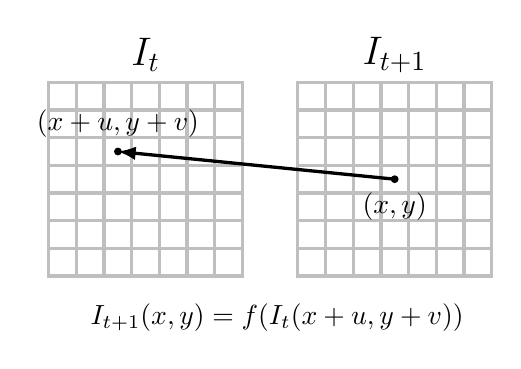
\begin{tikzpicture}[]
	\tikzset{box/.style={black, draw=black, fill=none, very thick, minimum height=4 em, minimum width=16 em}}

	\foreach \k in {0,...,1}
	{
		\foreach \i in {0,...,6}
		{
			\foreach \j in {0,...,6}
			{
				\node[box, fill=none, draw=gray!50, minimum height=1 em, minimum width=1 em] (l1-\i-\j-\k) at (\i em + 0.9 em * \k em, \j em) {};
			}
		}
	}

	\node at ([yshift=1.5 em]l1-3-6-0) {\Large $I_t$};
	\node at ([yshift=1.5 em]l1-3-6-1) {\Large $I_{t+1}$};
	\node at ([yshift=-2 em, xshift=-1.25 em]l1-0-0-1) {$I_{t+1}(x, y) = f(I_t(x + u, y + v))$};
	\node[shape=circle, inner sep=0.1 em, fill=black] at (l1-2-4-0) {};
	\node[shape=circle, inner sep=0.1 em, fill=black] at (l1-3-3-1) {};

	\draw[-latex, very thick] (l1-3-3-1.center) node[yshift=-1 em]{$(x,y)$} -- (l1-2-4-0.center) node[yshift=1 em]{$(x+u, y+v)$};

%	\node at ([yshift=1.5 em]l1-3-6-2) {\Large $I_t$};
%	\node at ([yshift=1.5 em]l1-3-6-3) {\Large $I_{t+1}$};

%	\node[shape=circle, inner sep=0.1 em, fill=black] at (l1-3-3-2) {};

%	\node[shape=circle, inner sep=0.1 em, fill=black] at (l1-3-3-3) {};
%	\node at ([yshift=-1 em]l1-3-3-2) {$(x, y)$};

%	\node at ([yshift=-1 em]l1-3-3-3) {$(x, y)$};

%	\node[draw=black, minimum height=3 em, minimum width=3 em, thick] at (l1-3-3-2) {};

%	\node at ([yshift=-2 em, xshift=-1.25 em]l1-0-0-3) {$I_{t+1}(x, y) = K(x,y) * P(x,y)$};
%	\node at ([yshift=-0.5 em]l1-3-1-2) {$P(x, y)$};


\end{tikzpicture}}
		\label{subfig:resampling_vector}}
	\subfloat[]{
		\resizebox{0.47\textwidth}{!}{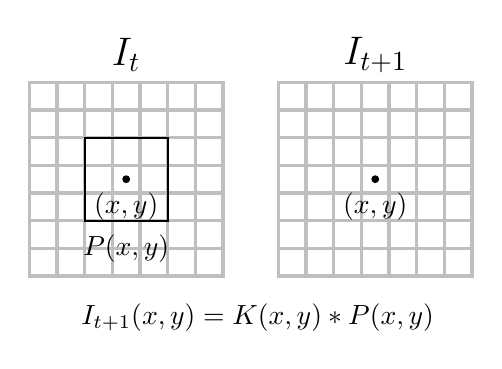
\begin{tikzpicture}[]
	\tikzset{box/.style={black, draw=black, fill=none, very thick, minimum height=4 em, minimum width=16 em}}

	\foreach \k in {0,...,1}
	{
		\foreach \i in {0,...,6}
		{
			\foreach \j in {0,...,6}
			{
				\node[box, fill=none, draw=gray!50, minimum height=1 em, minimum width=1 em] (l1-\i-\j-\k) at (\i em + 0.9 em * \k em, \j em) {};
			}
		}
	}

	\node at ([yshift=1.5 em]l1-3-6-0) {\Large $I_t$};
	\node at ([yshift=1.5 em]l1-3-6-1) {\Large $I_{t+1}$};

	\node[shape=circle, inner sep=0.1 em, fill=black] at (l1-3-3-0) {};

	\node[shape=circle, inner sep=0.1 em, fill=black] at (l1-3-3-1) {};
	\node at ([yshift=-1 em]l1-3-3-0) {$(x, y)$};

	\node at ([yshift=-1 em]l1-3-3-1) {$(x, y)$};

	\node[draw=black, minimum height=3 em, minimum width=3 em, thick] at (l1-3-3-0) {};

	\node at ([yshift=-2 em, xshift=-1.25 em]l1-0-0-1) {$I_{t+1}(x, y) = K(x,y) * P(x,y)$};
    \node at ([yshift=-0.5 em]l1-3-1-0) {$P(x, y)$};


\end{tikzpicture}}
		\label{subfig:resampling_kernel}}
	\caption{Representation of transformation-based approaches. (a) Vector-based with a bilinear interpolation. (b) Kernel-based applying transformations as a convolutional operation. Figure inspired by \cite{Reda2018}.}
	\label{fig:resampling}
\end{figure}
On the other side, in the kernel-based resampling, the $\mathcal{G}$ function predicts the kernel $\mathrm{K}(x, y)$ which is applied as a convolution operation using $\mathcal{T}$, as depicted in Figure~\ref{subfig:resampling_kernel} and is mathematically represented as follows:
\begin{equation}
\mathbf{Y}_{t+1}(x, y)=\mathrm{K}(x, y) * \mathbf{P}_{t}(x, y),
\end{equation} 
where $\mathrm{K}(x, y)\in\mathbb{R}^{NxN}$ is the 2D kernel predicted by the function $\mathcal{G}$ and $P_t(x,y)$ is an $N \times N$ patch centered at $(x,y)$. %Several future frame prediction approaches are kernel-based~\cite{Liu2017}. %add all the references

Combining kernel and vector-based resampling into a hybrid solution, Reda \textit{et al.}~\cite{Reda2018} proposed the \ac{SDC} module that synthesizes high-resolution images applying a learned per-pixel motion vector and kernel at a displaced location in the source image. Their 3D \ac{CNN} model trained on synthetic data and featuring the \ac{SDC} modules, reported promising predictions of a high-fidelity.

\subsubsection{Vector-based Resampling}
Bilinear models use multiplicative interactions to extract transformations from pairs of observations in order to relate images, such as \acp{GAE}~\cite{Memisevic2013a}. Inspired by these models, Michalski \textit{et al.} proposed the \ac{PGP}~\cite{Michalski2014} consisting of a recurrent pyramid of stacked \acp{GAE}. To the best of our knowledge, this was the first attempt to predict future frames in the affine transform space. Multiple \acp{GAE} are stacked to represent a hierarchy of transformations and capture higher-order dependencies. From the experiments on predicting frequency modulated sin-waves, authors stated that standard \acp{RNN} were outperformed in terms of accuracy. However, no performance comparison was conducted on videos. 
\begin{figure}[tbp]
	\centering
	\includegraphics[width=0.8\textwidth]{figures/videoprediction/methods/spatial_transformer.png}
	\caption{A representation of the spatial transformer module proposed by \cite{Jaderberg2015}. First, the localization network regresses the transformation parameters, denoted as $\theta$, from the input feature map $U$. Then, the grid generator creates a sampling grid from the predicted transformation parameters. Finally, the sampler produces the output map by sampling the input at the points defined in the sampling grid. Figure extracted from~\cite{Jaderberg2015}.}
	\label{fig:spatial_transformer}
\end{figure}

\vspace*{0.1cm}\noindent\textbf{Based on the \ac{ST} module \cite{Jaderberg2015}}: To provide spatial transformation capabilities to existing \acp{CNN}, Jaderberg \textit{et al.}~\cite{Jaderberg2015} proposed the \ac{ST} module. It regresses different affine transformation parameters for each input, to be applied as a single transformation to the whole feature map(s) or image(s). Moreover, it can be incorporated at any part of the \acp{CNN} and it is fully differentiable. The \ac{ST} module is the essence of vector-based resampling approaches for video prediction. As an extension, Patraucean \textit{et al.}~\cite{Patraucean2015} modified the grid generator to consider per-pixel transformations instead of a single dense transformation map for the entire image. They nested a \ac{LSTM}-based temporal encoder into a spatial \ac{AE}, proposing the AE-convLSTM-flow architecture. The prediction is generated by resampling the current frame with the flow-based predicted transformation. Using the components of the AE-convLSTM-flow architecture, Lu \textit{et al.}~\cite{Lu2017} assembled an extrapolation module which is unfolded in time for multi-step prediction. Their \ac{FSTN} features a novel loss function using the DeePSiM perceptual loss~\cite{Dosovitskiy2016} in order to mitigate blurriness. An exhaustive experimentation and ablation study was carried out, testing multiple combinations of loss functions. Also inspired by the \ac{ST} module for the volume sampling layer, Liu \textit{et al.} proposed the \ac{DVF} architecture~\cite{Liu2017}. It consists of a multi-scale flow-based \ac{ED} model originally designed for the video frame interpolation task, but also evaluated on a predictive basis reporting sharp results. Liang \textit{et al.}~\cite{Liang2017} use a flow-warping layer based on a bilinear interpolation. Finn \textit{et al.} proposed the \ac{STP} motion-based model~\cite{Finn2016} producing 2D affine transformations for bilinear sampling. Pursuing efficiency, Amersfoort \textit{et al.}~\cite{Amersfoort2017} proposed a \ac{CNN} designed to predict local affine transformations of overlapping image patches. Unlike the \ac{ST} module, authors estimated transformations of input frames off-line and at a patch level. As the model is parameter-efficient, it was unfolded in time for multi-step prediction. This resembles \acp{RNN} as the parameters are shared over time and the local affine transforms play the role of recurrent states.

\subsubsection{Kernel-based Resampling}
As a promising alternative to the vector-based resampling, recent approaches synthesize pixels by convolving input patches with a predicted kernel. However, convolutional operations are limited in learning spatial invariant representations of complex transformations. Moreover, due to their local receptive fields, global spatial information is not fully preserved. Using larger kernels would help to preserve global features, but in exchange for a higher memory consumption. Pooling layers are another alternative, but loosing spatial resolution. Preserving spatial resolution at a low computational cost is still an open challenge for future video frame prediction task. Transformation layers used in vector-based resampling~\cite{Jaderberg2015,Patraucean2015,Liu2017} enabled \acp{CNN} to be spatially invariant and also inspired kernel-based architectures.

\vspace*{0.1cm}\noindent\textbf{Inspired by the \ac{CDNA} module \cite{Finn2016}}: In addition to the \ac{STP} vector-based model, Finn \textit{et al.}~\cite{Finn2016} proposed two different kernel-based motion prediction modules outperforming previous approaches~\cite{Mathieu2016,Oh2015}, (1) the \ac{DNA} module predicting different distributions for each pixel and (2) the \ac{CDNA} module that instead of predicting different distributions for each pixel, it predicts multiple discrete distributions that are convolutionally applied to the input. While, \ac{CDNA} and \ac{STP} mask out objects that are moving in consistent directions, the \ac{DNA} module produces per-pixel motion. Similar to the \ac{CDNA} module, Klein~\textit{et al.} proposed the \ac{DCL}~\cite{Klein2015} for short-range weather prediction. Likewise, Brabandere \textit{et al.}~\cite{Brabandere2016} proposed the \ac{DFN} generating sample (for each image) and position-specific (for each pixel) kernels. This enabled sophisticated and local filtering operations in comparison with the \ac{ST} module, that is limited to global spatial transformations. Different to the \ac{CDNA} model, the \ac{DFN} uses a softmax layer to filter values of greater magnitude, thus obtaining sharper predictions. Moreover, temporal correlations are exploited using a parameter-efficient recurrent layer, much simpler than~\cite{Srivastava2015,Shi2015}. Exploiting adversarial training, Vondrick \textit{et al.} proposed a \ac{CGAN}-based model~\cite{Vondrick2017} consisting of a discriminator similar to~\cite{Vondrick2016}, and a \ac{CNN} generator featuring a transformer module inspired by the \ac{CDNA} model. Different from the \ac{CDNA} model, transformations are not applied recurrently on a per-frame basis. To deal with in-the-wild videos and make predictions invariant to camera motion, authors stabilized the input videos. However, no performance comparison with previous works has been conducted. Improving~\cite{Clark2019}, Luc \textit{et al.}~\cite{Luc2020} proposed the \ac{TRIVDGANFP} featuring a novel recurrent unit that computes the parameters of a transformation used to warp previous hidden states without any supervision. These \acp{TSRU} are generic modules and can replace any traditional recurrent unit in currently existent video prediction approaches.

\vspace*{0.1cm}\noindent\textbf{Object-centric representation}: Instead of focusing on the whole input, Chen \textit{et al.}~\cite{Chen2017} modeled individual motion of local objects, i.e. object-centered representations. Based on the \ac{ST} module and a pyramid-like sampling~\cite{He2015}, authors implemented an attention mechanism for object selection. Moreover, transformation kernels were generated dynamically as in the \ac{DFN}, to then apply them to the last patch containing an object. Although object-centered predictions is novel, performance drops when dealing with multiple objects and occlusions as the attention module fails to distinguish them correctly.

\subsection{Explicit Motion from Content Separation}
\label{subsc:two_stream}
Drawing inspiration from two-stream architectures for action recognition \cite{Simonyan2014}, and unconditioned video generation \cite{Tulyakov2018}, authors decided to factorize the video into content and motion to process each on a separate pathway. By factoring videos, the prediction is performed on a lower-dimensional temporal dynamics separately from the spatial layout. Although this makes end-to-end training difficult, splitting the prediction task into more tractable problems demonstrated good results. 
\begin{figure}[!tbp]
	\centering
	%\resizebox{\linewidth}{!}{
	\includegraphics[width=0.6\textwidth]{figures/videoprediction/methods/mcnet.png}
	\caption{\acf{MCNET} with Multi-scale Motion-Content Residuals. While the motion encoder captures the temporal dynamics in a sequence of image differences, the content encoder extracts meaningful spatial features from the last observed RGB frame. After that, the network computes motion-content features that are fed into the decoder to predict the next frame. Figure extracted from \cite{Villegas2017a}.}
	\label{fig:mcnet}
\end{figure}

The \ac{MCNET}~\cite{Villegas2017a} was the first end-to-end model in disentangling scene dynamics from the visual appearance, i.e. motion-content factorization. It proved better generalization capabilities and stable long-term predictions compared to~\cite{Srivastava2015,Mathieu2016}. In a similar fashion, yet working in a higher-level pose space, Denton \textit{et al.}~proposed \ac{DRNET}~\cite{Denton2017} using a novel adversarial loss ---it isolates the scene dynamics from the visual content, considered as the discriminative component--- to completely disentangle motion dynamics from content. Outperforming~\cite{Mathieu2016,Villegas2017a}, the \ac{DRNET} demonstrated a clean motion from content separation by reporting plausible long-term predictions on both synthetic and natural videos. To improve prediction variability, Liang \textit{et al.}~\cite{Liang2017} fused the future-frame and future-flow prediction into a unified architecture with a shared probabilistic motion encoder. Aiming to mitigate the ghosting effect in disoccluded regions, Gae \textit{et al.}~\cite{Gao2019} proposed a two-staged approach consisting of a separate computation of flow and pixel predictions. As they focused on inpainting occluded regions of the image using flow information, they improved results on disoccluded areas avoiding undesirable artifacts and enhancing sharpness. Wu \textit{et al.}~\cite{Wu2020} proposed a two-staged architecture that firstly predicts the static background to then, using this information, predict the moving objects in the foreground. Final output is generated through composition and by means of a video inpainting module. Reported predictions are quite accurate, yet performance was not contrasted with the latest video prediction models.

Although previous approaches disentangled motion from content, they have not performed an explicit decomposition of videos into primitive object representations. Addressing this issue, Hsieh \textit{et al.} proposed the \ac{DDPAE}~\cite{Hsieh2018} that decomposes videos into components featuring low-dimensional temporal dynamics. For instance, on the Moving MNIST dataset, \ac{DDPAE} first decomposes images into individual digits. After that, each digit is factorized into its visual appearance and spatial location, being the latter easier to predict. Although experiments were performed only on synthetic data, this model is a promising baseline encouraging predictive models to explore visual representation decomposition~\cite{Greff2017,Steenkiste2018,Steenkiste2019}.

\subsection{Conditioned on Extra Variables}
\label{subsec:m_condition}
Conditioning the prediction on extra variables such as vehicle odometry or robot state, among others, would narrow the prediction space. These variables have a direct influence on the dynamics of the scene, providing valuable information that facilitates the prediction task. For instance, the motion captured by a camera placed on the dashboard of an autonomous vehicle is directly influenced by the wheel-steering and acceleration. Without explicitly exploiting this information, we rely blindly on the model's capabilities to correlate the wheel-steering and acceleration with the perceived motion.

Following this paradigm, Oh \textit{et al.} first performed long-term video predictions conditioned by control inputs from Atari games~\cite{Oh2015}. Although the proposed \ac{ED}-based models reported very long-term predictions (+100), performance drops when dealing with small objects (e.g. bullets in Space Invaders) and uncertainty. However, $\ell_2$ loss leads to accurate and long-term predictions for deterministic synthetic videos, such as those extracted from Atari video games. Built on~\cite{Oh2015}, Chiappa \textit{et al.}~\cite{Chiappa2017} proposed alternative architectures and training schemes alongside an in-depth performance analysis for both short and long-term prediction. Similar to \cite{Oh2015}, Kaiser et al.~\cite{Kaiser2020} recently used a convolutional \ac{ED} to learn a world model of Atari games in a self-supervised fashion. This is part of their model-based \ac{RL} approach called \ac{SIMPLE} focused on learning to play Atari games. In the experiments, \ac{SIMPLE} outperforms previous model-free algorithms requiring only 1-2 hours of in-game interactions. Similar model-based control from visual inputs performed well in restricted scenarios~\cite{Fragkiadaki2016}, but was inadequate for unconstrained environments.

Deterministic approaches are unable to deal with natural videos in the absence of control variables. To address this limitation, the models proposed by Finn et al.~\cite{Finn2016} successfully made predictions on natural images, conditioned on the robot state and robot-object interactions performed in a controlled scenario. These models predict per-pixel transformations conditioned by the previous frame, to finally combine them using a composition mask. They outperformed~\cite{Oh2015,Mathieu2016} on both conditioned and unconditioned predictions, however the quality of long-term predictions degrades over time because of the blurriness caused by the \ac{MSE} loss function. Furthermore, Dosovitskiy \textit{et al.}~\cite{Dosovitskiy2017} proposed a sensorimotor control model which enables interaction in complex and dynamic \ac{3D} environments. The approach is a \ac{RL}-based technique, with the difference that instead of building upon a monolithic state and a scalar reward, the authors consider high-dimensional input streams, such as raw visual input, alongside a stream of measurements or player statistics. Although the outputs are future measurements instead of visual predictions, it was proven that using multivariate data benefits decision-making over conventional scalar reward approaches. The synergy between model-based \ac{RL}~\cite{Hafner2019,Kaiser2020,Hafner2020} and video prediction is well defined as the latter aims to model an accurate representation of high-dimensional environments, while the former uses the learned world models as a context for decision-making.

\subsection{In the High-level Feature Space}
\label{subsec:m_high_level}
Despite the vast work on video prediction models, there is still room for improvement in natural video prediction. To deal with the curse of dimensionality, authors reduced the prediction space to higher-level representations, such as semantic and instance segmentation, and human pose. Since the pixels are categorical, the semantic space greatly simplifies the prediction task, yet unexpected deformations in semantic maps and disocclusions, i.e. initially occluded scene entities become visible, induce uncertainty.
%%%AAA: Disocclusions? 
However, high-level prediction spaces are more tractable and constitute good intermediate representations. By bypassing the prediction in the raw pixel space, models reported longer-term and more accurate predictions.

\subsubsection{Semantic Segmentation}
By decomposing the visual scene into semantic entities, such as pedestrians, vehicles and obstacles, the output space is narrowed to high-level scene properties. This intermediate representation represents a more tractable space as pixel values of a semantic map are categorical. In other words, scene dynamics are modeled at the semantic entity level. This has encouraged authors to (1) leverage future prediction to improve parsing results~\cite{Jin2017} and (2) directly predict segmentation maps into the future~\cite{Luc2017, Luc2018, Luc2019}.
\begin{figure*}[tbp]
	\centering
	\includegraphics[width=\textwidth]{figures/videoprediction/methods/student_teacher.png}
	\caption{Two-staged method proposed by Chiu \textit{et al.} \cite{Chiu2019}. In the upper half, the student network consists on an \ac{ED}-based architecture featuring a 3D convolutional forecasting module. It performs the forecasting task guided by an additional loss generated by the teacher network (represented in the lower half). Figure extracted from \cite{Chiu2019}.}
	\label{fig:student_teacher}
\end{figure*}

Exploring the scene parsing in future frames, Jin \textit{et al.} proposed the \ac{PEARL} framework~\cite{Jin2017} which was the first to explore the potential of a \ac{GAN}-based predictive model to improve per-pixel segmentation. Specifically, this framework conducts two complementary predictive learning tasks. Firstly, it captures the temporal context from input data by using a single-frame prediction network. Then, these temporal features are embedded into a frame parsing network through a transform layer for generating per-pixel future segmentations. Although the prediction model was not compared with existing approaches, \ac{PEARL} outperforms the traditional parsing methods by generating temporally consistent segmentations. In a similar fashion, Luc \textit{et al.}~\cite{Luc2017} extended the ms\ac{CNN} model of~\cite{Mathieu2016} to the novel task of predicting semantic segmentations of future frames, using softmax pre-activations instead of raw pixels as input. The use of intermediate features or higher-level data as input is a common practice in the video prediction performed in the high-level feature space. Some authors refer to this type or input data as percepts. Luc \textit{et al.} explored different combinations of loss functions, inputs (using RGB information alongside percepts), and outputs (autoregressive and batch models). Results on short, medium and long-term predictions are sound, however, the models are not end-to-end and they do not capture explicitly the temporal continuity across frames. To address this limitation and extending~\cite{Jin2017}, Jin \textit{et al.} first proposed a model for jointly predicting motion flow and scene parsing~\cite{Jin2017a}. Flow-based representations implicitly draw temporal correlations from the input data, thus producing temporally consistent segmentations. Per-pixel accuracy improved when segmenting small objects, e.g. pedestrians and traffic signs, which are more likely to vanish in long-term predictions. Similarly, except that time dimension is modeled with a \acp{LSTM} instead of motion flow estimation, Nabavi \textit{et al.} proposed a simple bidirectional \ac{ED}-\ac{LSTM}~\cite{Nabavi2018} using segmentation masks as input. Although the literature on knowledge distillation~\cite{Ba2014,Hinton2015} stated that softmax pre-activations carry more information than class labels, this model outperforms~\cite{Jin2017a,Luc2017} on short-term predictions.

Using motion flow estimation alongside \ac{LSTM}-based temporal modeling, Terwilliger \textit{et al.}~\cite{Terwilliger2019} proposed a novel method performing a \ac{LSTM}-based feature-flow aggregation. Authors further simplify the semantic space by disentangling motion from semantic entities~\cite{Villegas2017a}, achieving low overhead and efficiency. Therefore, they segment the current frame and perform future optical flow prediction, which are finally combined with a novel end-to-end warp layer. An improvement on short-term predictions was reported over previous works~\cite{Luc2017,Jin2017a}, yet performing worse on mid-term predictions. Similar to \cite{Terwilliger2019}, F2MF model~\cite{Saric2020} predict semantic segmented frames by wrapping past convolutional features into the future using a regressed dense displacement field. To deal with disocclusions, authors complemented the main model with a classical feature-to-feature forecast module similar to~\cite{Chiu2019,Luc2018}. F2MF outperformed previous works on the CityScapes dataset without using structure information~\cite{Vora2018} or precomputed optical flow~\cite{Terwilliger2019}.

A different approach was proposed by Vora \textit{et al.}~\cite{Vora2018} which first incorporated structure information to predict future 3D segmented point clouds. Their geometry-based model consists of several derivable sub-modules: (1) the pixel-wise segmentation and depth estimation modules which are jointly used to generate the \ac{3D} segmented point cloud of the current RGB frame; and (2) an \ac{LSTM}-based module trained to predict future camera ego-motion trajectories. The future \ac{3D} segmented point clouds are obtained by transforming the previous point clouds with the predicted ego-motion. Their short-term predictions improved the results of \cite{Luc2017}, however, the use of structure information for longer-term predictions is not clear.

The main disadvantage of two-staged, i.e. not end-to-end, approaches~\cite{Luc2017,Jin2017a,Nabavi2018,Vora2018,Terwilliger2019} is that their performance is constrained by external supervisory signals, e.g. optical flow~\cite{Revaud2015}, segmentation~\cite{Zhao2017a} and intermediate features or percepts~\cite{Yu2017}. Breaking this trend, Chiu \textit{et al.}~\cite{Chiu2019} first solved both the semantic segmentation and forecasting problems in a single end-to-end trainable model by using raw pixels as input. This \ac{ED} architecture is based on two networks: the student, performing the forecasting task, and the teacher guiding the student using a novel knowledge distillation loss. An in-depth ablation study was performed, validating the performance of the \ac{ED} architectures as well as the 3D convolution used for capturing the temporal scale instead of a \ac{LSTM} or \ac{CONVLSTM}, as in previous works. 

Avoiding the flood of deterministic models, Bhattacharyya \textit{et al.} proposed a Bayesian formulation of the ResNet model in a novel architecture to capture model and observation uncertainty~\cite{Bhattacharyya2019}. As a main contribution, their dropout-based Bayesian approach leverages synthetic likelihoods~\cite{Rosca2017} to encourage prediction diversity and deal with multi-modal outcomes. Since Cityscapes sequences have been recorded in the frame of reference of a moving vehicle, authors conditioned the predictions on vehicle odometry. 

\subsubsection{Instance Segmentation}
While great strides have been made in predicting future segmentation maps, the authors attempted to make predictions at a semantically richer level, i.e. future prediction of semantic instances. Predicting future instance-level segmentations is a challenging and weakly unexplored task. This is because instance labels are inconsistent and variable in number across the frames in a video sequence. Since the representation of semantic segmentation prediction models is of fixed-size, they cannot directly address semantics at the instance level.

To overcome this limitation and introducing the novel task of predicting instance segmentations, Luc \textit{et al.}~\cite{Luc2018} predict fixed-sized feature pyramids, i.e. features at multiple scales, used by the Mask R-CNN~\cite{He2017} network. The combination of dilated convolutions and multi-scale, efficiently preserve high-resolution details improving the results over previous methods~\cite{Luc2017}. To further improve predictions, Sun \textit{et al.}~\cite{Sun2019} focused on modeling not only the spatio-temporal correlations between the pyramids, but also the intrinsic relations among the feature layers inside them. That is, enriching the contextual information using the proposed \acp{CPCONVLSTM}. Although the authors have not shown any long-term predictions nor compared with semantic segmentation models, their approach is the state of the art in the task of predicting instance segmentations.

\subsubsection{Other High-level Spaces}
Although semantic and instance segmentation spaces were the most used in video prediction, other high-level spaces such as human pose and keypoints, represent a promising avenue.

\vspace*{0.1cm}\noindent\textbf{Human Pose}: As the human pose is a low-dimensional and interpretable structure, it represents a cheap supervisory signal for predictive models. This has fostered pose-guided prediction methods, in which pixel-level predictions are conditioned by intermediate representations of human poses. However, most of these methods are limited to videos with human presence.

From a supervised prediction of human poses, Villegas \textit{et al.}~\cite{Villegas2017} regress future frames through analogy making~\cite{Reed2015}. Although background is not considered in the prediction, authors compared the model against~\cite{Shi2015,Mathieu2016} reporting long-term results. To make the model unsupervised on the human pose, Wichers \textit{et al.}~\cite{Wichers2018} adopted different training strategies: end-to-end prediction minimizing the $\ell_2$ loss, and through analogy making, constraining the predicted features to be close to the outputs of the future encoder. Different from~\cite{Villegas2017}, predictions are made in the feature space. As a probabilistic alternative, Walker \textit{et al.}~\cite{Walker2017} fused a \ac{CVAE}-based probabilistic pose predictor with a \ac{GAN}. While the probabilistic predictor enhances the diversity in the predicted poses, the adversarial network ensures prediction realism. As this model struggles with long-term predictions, Fushishita \textit{et al.}~\cite{Fushishita2019} addressed long-term video prediction of multiple outcomes avoiding the error accumulation and vanishing gradients by using a unidimensional \ac{CNN} trained in an adversarial fashion. To enable multiple predictions, they have used additional inputs ensuring trajectory and behavior variability at a human pose level. To better preserve the visual appearance in the predictions than~\cite{Lee2018,Villegas2017a,Villegas2017}, Tang \textit{et al.}~\cite{Tang2019} firstly predict human poses using a \ac{LSTM}-based model to then synthesize pose-conditioned future frames using a combination of different networks: a global \ac{GAN} modeling the time-invariant background alongside a coarse human pose, a local \ac{GAN} refining the coarse-predicted human pose, and a 3D-\ac{AE} to ensure temporal consistency across frames. 
%%%(solved) AAA: You should explain why you find this interesting: explained in detail below

\vspace*{0.1cm}\noindent\textbf{Keypoint-based representations}: The keypoint coordinate space is a meaningful, tractable and structured representation for prediction, ensuring stable learning. It enforces model's internal representation to contain object-level information. This leads to better results on tasks requiring object-level understanding such as, trajectory prediction, action recognition and reward prediction. As keypoints are a natural representation of dynamic objects, Minderer \textit{et al.}~\cite{Minderer2019} reformulated the prediction task in the keypoint coordinate space. They proposed an \ac{AE} architecture with a bottleneck consisting of a \ac{VRNN} that predicts dynamics in the keypoint space. Although this model qualitatively outperforms the \ac{SVG}~\cite{Denton2018}, \ac{SAVP}~\cite{Lee2018} and \ac{EPVA}~\cite{Wichers2018} models, the quantitative evaluation reported similar results.

\subsection{Incorporating Uncertainty}
\label{subsec:m_uncertainty}
Although high-level representations significantly reduce the prediction space, the underlying distribution still has multiple modes. In other words, different plausible outcomes would be equally probable for the same input. Addressing multimodal distributions is not straightforward for regression and classification approaches, as they regress to the mean and aim to discretize a continuous high-dimensional space, respectively. To deal with the inherent unpredictability of natural videos, some works introduced latent variables into existing deterministic models or directly relied on generative models such as \acp{GAN} and \acp{VAE}.

Inspired by \ac{DVF}, Xue \textit{et al.}~\cite{Xue2016} proposed a \ac{CVAE}-based~\cite{Kingma2014,Yan2016} multi-scale model featuring a novel cross convolutional layer trained to regress the difference image or Eulerian motion~\cite{Wu2012}. Background on natural videos is not uniform, however the model implicitly assumes that the difference image would accurately capture the movement in foreground objects. Introducing latent variables into a convolutional \ac{AE}, Goroshin \textit{et al.}~\cite{Goroshin2015a} proposed a probabilistic model for learning linearized feature representations to linearly extrapolate the predicted frame in a feature space. Uncertainty is introduced to the loss by using a cosine distance as an explicit curvature penalty. Authors focused on evaluating the linearization properties, yet the model was not contrasted to previous works. Extending~\cite{Xue2016,Walker2016}, Fragkiadaki \textit{et al.}~\cite{Fragkiadaki2017} proposed several architectural changes and training schemes to handle marginalization over stochastic variables, such as sampling from the prior and variational inference. Their stochastic \ac{ED} architecture predicts future optical flow, i.e., dense pixel motion field, used to spatially transform the current frame into the next frame prediction. To introduce uncertainty in predictions, the authors proposed the k-best-sample-loss (MCbest) that draws $K$ outcomes penalizing those similar to the ground-truth. 

Incorporating latent variables into the deterministic \ac{CDNA} architecture for the first time, Babaeizadeh \textit{et al.} proposed the \ac{SV2P}~\cite{Babaeizadeh2018} model handling natural videos. Their time-invariant posterior distribution is approximated from the entire input video sequence. Moreover, with the explicit modeling of uncertainty using latent variables, the deterministic \ac{CDNA} model is outperformed. By combining a standard deterministic architecture (\ac{LSTM}-\ac{ED}) with stochastic latent variables, Denton \textit{et al.} proposed the \ac{SVG} network~\cite{Denton2018}. Different from \ac{SV2P}, the prior is sampled from a time-varying posterior distribution, i.e. it is a learned-prior instead of fixed-prior sampled from the same distribution. Most of the \acp{VAE} use a fixed Gaussian as a prior, sampling randomly at each time step. Exploiting the temporal dependencies, a learned-prior predicts high variance in uncertain situations, and a low variance when a deterministic prediction suffices. The \ac{SVG} model is easier to train and reported sharper predictions in contrast to~\cite{Babaeizadeh2018}. Built upon \ac{SVG}, Villegas \textit{et al.}~\cite{Villegas2019} implemented a baseline to perform an in-depth empirical study on the importance of the inductive bias, stochasticity, and model's capacity in the video prediction task. Different from previous approaches, Henaff \textit{et al.} proposed the \ac{EEN}~\cite{Henaff2017} that incorporates uncertainty by feeding back the residual error ---the difference between the ground truth and the deterministic prediction--- encoded as a low-dimensional latent variable. In this way, the model implicitly separates the input video into deterministic and stochastic components.

On the one hand, latent variable-based approaches cover the space of possible outcomes, yet predictions lack of realism. On the other hand, \acp{GAN} struggle with uncertainty, but predictions are more realistic. Searching for a trade-off between \acp{VAE} and \acp{GAN}, Lee \textit{et al.}~\cite{Lee2018} proposed the \ac{SAVP} model. It was the first to combine latent variable models with \acp{GAN} to improve variability in video predictions, while maintaining realism. Under the assumption that blurry predictions of \acp{VAE} are a sign of underfitting, Castrejon \textit{et al.} extended the \acp{VRNN} to leverage a hierarchy of latent variables and better approximate data likelihood~\cite{Castrejon2019}. Although the backpropagation through a hierarchy of conditioned latents is not straightforward, several techniques alleviated this issue such as, KL beta warm-up, dense connectivity pattern between inputs and latents, and \acp{LVAE} \cite{Sonderby2016}. As most of the probabilistic approaches fail in approximating the true distribution of future frames, Pottorff \textit{et al.}~\cite{Pottorff2019} reformulated the video prediction task without making any assumption about the data distribution. They proposed the \ac{ILE} that enables exact maximum likelihood learning of video sequences, by combining an invertible neural network \cite{Kingma2018}, also known as reversible flows, and a linear time-invariant dynamic system. The \ac{ILE} handles nonlinear motion in the pixel space and scales better to longer-term predictions compared to adversarial models~\cite{Mathieu2016}. Also based on Glow model~\cite{Kingma2018} and sharing goals with~\cite{Pottorff2019}, VideoFlow~\cite{Kumar2020} approaches exact likelihood maximization using normalized flows through invertible transformations. These flow-based architectures present several advantages such as, exact log-likelihood evaluation and faster sampling than autoregressive models, while still producing high-quality long-term and stochastic predictions.

While previous variational approaches~\cite{Denton2018,Lee2018} focused on predicting a single frame of low resolution in restricted, predictable or simulated datasets, Hu \textit{et al.}~\cite{Hu2020} jointly predict full-frame ego-motion, static scene, and object dynamics on complex real-world urban driving. Featuring a novel spatio-temporal module, their five-component architecture learns rich representations that incorporate both local and global spatio-temporal context. The model outperformed existing spatio-temporal architectures, by predicting semantic segmentation, depth and optical flow. However, no performance comparison with~\cite{Denton2018,Lee2018} has been carried out.

\begin{landscape}
	\ra{1.12}
	\label{table:methods}
	\footnotesize
	\begin{ThreePartTable}
		\setlength\LTleft{0pt}
		\setlength\LTright{0pt}
		\begin{longtable}[t]{@{\extracolsep{\fill}}lcccccccclcc@{}}
			\caption{Summary of video prediction models (\textbf{c}: \textbf{c}onvolutional; \textbf{r}: \textbf{r}ecurrent; \textbf{v}: \textbf{v}ariational; \textbf{ms}: \textbf{m}ulti-\textbf{s}cale; \textbf{st}: \textbf{st}acked; \textbf{bi}: \textbf{bi}directional; \textbf{P}: \textbf{P}ercepts; \textbf{M}: \textbf{M}otion; \textbf{PL}: \textbf{P}erceptual \textbf{L}oss; \textbf{AL}: \textbf{A}dversarial \textbf{L}oss; \textbf{S}/\textbf{R}: using \textbf{S}ynthetic/\textbf{R}eal datasets; \textbf{SS}: \textbf{S}emantic \textbf{S}egmentation; \textbf{D}: \textbf{D}epth; \textbf{S}: \textbf{S}tate; \textbf{Po}: \textbf{Po}se; \textbf{O}: \textbf{O}dometry; \textbf{IS}: \textbf{I}nstance \textbf{S}egmentation; \textbf{MS}: \textbf{M}ulti-\textbf{S}tep prediction; \textbf{npf}: num. of \textbf{p}redicted \textbf{f}rames, $\0$ 1-5, $\0\0$ 5-10, $\0\0\0$ 10-100, $\0\0\0\0$ over 100 frames; \textbf{ood}: tested on \textbf{o}ut-\textbf{o}f-\textbf{d}omain tasks).} \\
			\toprule
			& & & & \multicolumn{4}{c}{\textbf{details}} & \multicolumn{3}{c}{\textbf{evaluation}} & \\
			\cmidrule(lr){5-8} \cmidrule(lr){9-11} 
			\textbf{method} & \textbf{year} & \textbf{architecture} & \textbf{datasets (train, valid, test)} & \textbf{input} & \textbf{output} & \textbf{MS} & \textbf{loss function} & \textbf{S/R} & \textbf{npf} & \textbf{ood} & \textbf{code} \\
			\midrule
			\endhead
			\multicolumn{12}{c}{\textbf{Direct Pixel Synthesis}} \\
			\midrule
			Ranzato \textit{et al.} \cite{Ranzato2014} & \num{2014} & r\ac{CNN} & \cite{Soomro2012,Cadieu2012} & RGB & RGB & \xmark & $\ac{CE}$ & R & $\0$ & \xmark & \xmark \\ %done
			Srivastava \textit{et al.} \cite{Srivastava2015} & \num{2015} & \ac{LSTM}-\ac{AE} & \cite{Soomro2012,Kuehne2011,Srivastava2015,Karpathy2014} & RGB,P & RGB & \checkmark & $\ac{CE},\ell_2$ & SR & $\0\0\0$ & \checkmark & \checkmark \\ %Not end-to-end
			\ac{PGN} \cite{Lotter2015} & \num{2015} & \ac{LSTM}-c\ac{ED} & \cite{Sutskever2008} & RGB & RGB & \xmark & $\ac{MSE},AL$ & S & $\0$ &  \xmark & \xmark \\
			Shi \textit{et al.} \cite{Shi2015} & \num{2015} & c\ac{LSTM} & \cite{Srivastava2015} & RGB & RGB & \xmark & $\ac{CE}$ & S & $\0\0\0$ &  \checkmark & \xmark \\ 
			BeyondMSE \cite{Mathieu2016} & \num{2016} &  ms\ac{CNN} & \cite{Soomro2012,Karpathy2014} & RGB & RGB & \checkmark & $\ell_1,\ac{GDL},AL$ & R & $\0\0$ & \xmark & \checkmark \\ 
			PredNet \cite{Lotter2017} & \num{2017} &  st\acp{LSTM} & \cite{Geiger2013,Dollar2009,Ionescu2014,Santana2016} & RGB & RGB & \checkmark & $\ell_1$,$\ell_2$ & SR & $\0\0$ & \checkmark & \checkmark \\ %done
			ContextVP \cite{Byeon2018} & \num{2018} & \ac{MDLSTM} &  \cite{Soomro2012,Geiger2013,Dollar2009,Ionescu2014} & RGB & RGB & \checkmark & $\ell_1,\ac{GDL}$ & R & $\0\0$ & \xmark & \xmark \\
			\ac{FRNN} \cite{Oliu2018} & \num{2018} & c\acs{GRU}-\ac{AE} & \cite{Srivastava2015,Schuldt2004,Soomro2012} & RGB & RGB & \checkmark & $\ell_1$ & SR & $\0\0\0$ & \xmark & \checkmark \\
			\ac{E3DLSTM} \cite{Wang2019b} & \num{2019} & r\ac{3D}-\ac{CNN} & \cite{Srivastava2015,Schuldt2004,Zhang2017a,Goyal2017} & RGB & RGB & \checkmark & $\ell_1,\ell_2,\ac{CE}$ & SR & $\0\0\0$ & \checkmark & \checkmark \\
			Kwon \textit{et al.} \cite{Kwon2019} & \num{2019} & cycleGAN & \cite{Geiger2013,Dollar2009,Soomro2012,Luo2017a,Ravanbakhsh2017} & RGB & RGB & \checkmark & $\ell_1,\acs{LOG},AL$ & R & $\0\0\0$ & \xmark & \xmark \\
			Znet \cite{Zhang2019} & \num{2019} & c\ac{LSTM} & \cite{Srivastava2015,Schuldt2004} & RGB & RGB & \checkmark & $\ell_2,BCE,AL$ & SR & $\0\0\0$ & \xmark & \xmark \\
			VPGAN \cite{Hu2019} & \num{2019} & \ac{GAN} & \cite{Ebert2017,Schuldt2004} & RGB,Z & RGB & \checkmark & $\ell_1,L_{cycle},AL$ & R & $\0\0\0$ & \xmark & \xmark \\
			Jin \textit{et al.}\cite{Jin2020} & \num{2020} & c\ac{ED}-\ac{GAN} & \cite{Schuldt2004,Dollar2009,Geiger2013,Ebert2017} & RGB & RGB & \checkmark & $\ell_2,\ac{GDL},AL$ & R & $\0\0\0$ & \xmark & \xmark \\
			Shouno \textit{et al.}\cite{Shouno2020} & \num{2020} & \ac{GAN} & \cite{Dollar2009,Geiger2013} & RGB & RGB & \checkmark & $L_p,AL,PL$ & R & $\0\0\0$ & \xmark & \xmark \\
			\ac{CREVNET}\cite{Yu2020} & \num{2020} & \ac{3D}-c\ac{ED} & \cite{Srivastava2015,Dollar2009,Geiger2013,traffic4cast} & RGB & RGB & \checkmark & $\ac{MSE}$ & SR & $\0\0\0$ & \checkmark & \checkmark \\
			\midrule
			\multicolumn{12}{c}{\textbf{Using Explicit Transformations}} \\
			\midrule
			\ac{PGP} \cite{Michalski2014} & \num{2014} & st-r\acp{GAE} & \cite{Memisevic2013,Sutskever2008} & RGB & RGB & \checkmark & $\ell_2$ & SR & $\0$ & \xmark & \xmark \\ 
			Patraucean \textit{et al.} \cite{Patraucean2015} & \num{2015} & \ac{LSTM}-c\ac{AE} & \cite{Srivastava2015,Kuehne2011,Santner2010,Vezzani2010} & RGB & RGB & \xmark & $\ell_2,\ell_\delta$ & SR & $\0$ & \checkmark & \checkmark \\
			\ac{DFN} \cite{Brabandere2016} & \num{2016} & r-c\ac{ED} & \cite{Soomro2012,Srivastava2015} & RGB & RGB & \checkmark & $B\ac{CE}$ & SR & $\0\0\0$ & \checkmark & \checkmark \\
			Amersfoort \textit{et al.} \cite{Amersfoort2017} & \num{2017} & \ac{CNN} & \cite{Soomro2012,Srivastava2015} & RGB & RGB & \checkmark & $\ac{MSE}$ & SR & $\0\0$ & \xmark & \xmark \\
			\ac{FSTN} \cite{Lu2017} & \num{2017} & \ac{LSTM}-c\ac{ED} & \cite{Soomro2012,Srivastava2015,Santner2010,Vezzani2010,Karpathy2014} & RGB & RGB & \checkmark & $\ell_2,\ell_\delta,PL$ & SR & $\0\0\0$ & \xmark & \xmark \\
			Vondrick \textit{et al.} \cite{Vondrick2017} & \num{2017} & \ac{CGAN} & \cite{Thomee2016} & RGB & RGB & \checkmark & $\ac{CE},AL$ & R & $\0\0\0$ & \checkmark & \xmark \\
			Chen \textit{et al.} \cite{Chen2017} & \num{2017} & r\ac{CNN}-\ac{ED} & \cite{Soomro2012,Srivastava2015} & RGB & RGB & \checkmark & $CE,\ell_2,\ac{GDL},AL$ & SR & $\0\0$ & \xmark & \xmark \\
			\ac{DVF} \cite{Liu2017} & \num{2017} & ms-c\ac{ED} & \cite{Soomro2012,Idrees2017} & RGB & RGB & \checkmark & $\ell_1, \ac{TV}$ & R & $\0$ & \checkmark & \checkmark \\
			SDC-Net \cite{Reda2018} & \num{2018} & \ac{CNN} & \cite{Dollar2009,Abu-El-Haija2016} & RGB,M & RGB & \checkmark & $\ell_1,PL$ & SR & $\0\0$ & \checkmark & \xmark \\
			\ac{TRIVDGANFP} \cite{Luc2020} & \num{2020} & DVD-\ac{GAN} & \cite{Soomro2012,Ebert2017,Carreira2018} & RGB & RGB & \checkmark & $L_{hinge}$\cite{Liang2017} & R & $\0\0\0$ & \xmark & \xmark \\
			\midrule
			\multicolumn{12}{c}{\textbf{Explicit Motion from Content Separation}} \\
			\midrule
			\ac{MCNET} \cite{Villegas2017a} & \num{2017} & \ac{LSTM}-c\ac{ED} & \cite{Soomro2012,Karpathy2014,Gorelick2007,Schuldt2004} & RGB & RGB & \checkmark & $\ell_p,\ac{GDL},AL$ & R & $\0\0\0$ & \xmark & \checkmark \\
			Dual-GAN \cite{Liang2017} & \num{2017} & \ac{VAE}-\ac{GAN} & \cite{Soomro2012,Dollar2009,Geiger2013,Idrees2017} & RGB & RGB & \checkmark & $\ell_1,KL,AL$ & R & $\0\0$ & \xmark & \xmark \\
			\ac{DRNET} \cite{Denton2017} & \num{2017} & \ac{LSTM}-\ac{ED} & \cite{Srivastava2015,LeCun2004,Song2017,Schuldt2004} & RGB & RGB & \checkmark & $\ell_2,\ac{CE},AL$ & SR & $\0\0\0\0$ & \checkmark & \checkmark \\
			DPG \cite{Gao2019} & \num{2019} & c\ac{ED} & \cite{Dollar2009,Menze2015,Janai2018} & RGB & RGB & \checkmark & $\ell_p,\ac{TV},PL,CE$ & SR & $\0\0$ & \xmark & \xmark \\
			%Wu \textit{et al.} \cite{Wu2020} & 2020 & \cite{Denton2017,Villegas2017,Luo2017} & c\ac{gan} & \cite{Geiger2013,Cordts2016} & RGB,SS,IS,M\tnote{2} & RGB & \checkmark & - & R & - & - & - \\
			\midrule
			\multicolumn{12}{c}{\textbf{Conditioned on Extra Variables}} \\
			\midrule
			Oh \textit{et al.} \cite{Oh2015} & \num{2015} & r\ac{ED} & \cite{Bellemare2013} & RGB,A & RGB & \checkmark & $\ell_2$ & S & $\0\0\0\0$  & \checkmark & \checkmark \\ %Prediction over 100 frames in ALE. Tested for control in robot environment. Eval. metric: MSE. Transform space conditioned on actions
			Finn \textit{et al.} \cite{Finn2016} & \num{2016} & st-c\acp{LSTM} & \cite{Finn2016,Ionescu2014} & RGB,A,S & RGB & \checkmark & $\ell_2$ & R & $\0\0\0$ & \xmark & \checkmark \\ %trained up to 8 time-steps and tested up to 18. PSNR and SSIM
			\midrule
			\multicolumn{12}{c}{\textbf{In the High-level Feature Space}} \\
			\midrule
			Villegas \textit{et al.} \cite{Villegas2017} & \num{2017} & \ac{LSTM}-c\ac{ED} & \cite{Ionescu2014,Zhang2013} & RGB,Po & RGB,Po & \checkmark & $\ell_2,PL,AL$\cite{Dosovitskiy2016} & R & $\0\0\0\0$ & \checkmark & \xmark \\
			\ac{PEARL} \cite{Jin2017} & \num{2017} & c\ac{ED} & \cite{Cordts2016,Brostow2008} & RGB & SS & \xmark & $\ell_2,AL$ & R & $\0$ & \checkmark & \xmark \\ %GAN
			S2S \cite{Luc2017} & \num{2017} &  ms\ac{CNN} & \cite{Cordts2016,Brostow2008} & P & SS & \checkmark & $\ell_1,\ac{GDL},AL$ & R & $\0\0\0$ & \xmark & \checkmark \\ %Metrics: IoU, PSNR, SSIM. Dilation-10 softmax pre-activation
			Walker \textit{et al.} \cite{Walker2017} & \num{2017} &  \ac{CVAE} & \cite{Soomro2012,Zhang2013} & RGB,Po & RGB & \checkmark & $\ell_2,\ac{CE},KL,AL$ & R & $\0\0\0$ & \checkmark & \xmark  \\ %32 frame prediction
			Jin et al. \cite{Jin2017a} & \num{2017} &  c\ac{ED} & \cite{Cordts2016,Santana2016} & RGB,P & SS,M & \checkmark & $\ell_1,\ac{GDL},\ac{CE}$ & R & $\0\0\0$ & \checkmark & \xmark \\ % metrics: mIoU and average enpoint error (EPE)
			\ac{EPVA} \cite{Wichers2018} & \num{2018} & \ac{LSTM}-\ac{ED} & \cite{Ionescu2014} & RGB & RGB & \checkmark & $\ell_2,AL$ & SR & $\0\0\0\0$ & \checkmark & \checkmark \\ %127 frames into the future for tests. 32 for training
			Nabavi \textit{et al.} \cite{Nabavi2018} & \num{2018} & bi\ac{LSTM}-c\ac{ED} & \cite{Cordts2016} & P & SS & \checkmark & $\ac{CE}$ & R & $\0\0$ & \xmark & \xmark \\
			F2F \textit{et al. }\cite{Luc2018} & \num{2018} & st-ms\ac{CNN} & \cite{Cordts2016} & P & P,SS,IS & \checkmark & $\ell_2$ & R & $\0\0\0$ & \checkmark & \checkmark \\
			Vora \textit{et al.} \cite{Vora2018} & \num{2018} & \ac{LSTM} & \cite{Cordts2016} & ego-M & ego-M & \xmark & $\ell_1$ & R & $\0$ & \checkmark & \xmark \\ %up to 3 frame prediction
			Chiu \textit{et al.} \cite{Chiu2019} & \num{2019} & 3D-c\ac{ED} & \cite{Cordts2016,Huang2018a} & RGB & SS & \xmark & $\ac{CE},\ac{MSE}$ & R & $\0\0$ & \xmark & \xmark \\
			Bayes-WD-SL \cite{Bhattacharyya2019} & \num{2019} & bayesResNet & \cite{Cordts2016} & SS,O & SS & \checkmark & $KL$ & SR & $\0\0\0$ & \checkmark & \checkmark \\
			Sun \textit{et al.} \cite{Sun2019} & \num{2019} &  st-ms-c\ac{LSTM} & \cite{Cordts2016,Seguin2016} & P & P,IS & \checkmark & $\ell_2$,\cite{He2017} & R & $\0\0$ & \xmark & \xmark  \\ 
			Terwilliger \textit{et al.} \cite{Terwilliger2019} & \num{2019} & M-c\ac{LSTM} & \cite{Cordts2016} & RGB,P & SS & \checkmark & $\ac{CE},\ell_1$ & R & $\0\0\0$ & \xmark & \checkmark \\
			Struct-\ac{VRNN} \cite{Minderer2019} & \num{2019} & c\ac{VRNN} & \cite{Zhan2019,Ionescu2014} & RGB & RGB & \checkmark & $\ell_2,KL$ & SR & $\0\0$ & \checkmark & \checkmark \\
			F2MF \cite{Saric2020} & \num{2020} & \cite{Terwilliger2019} & \cite{Cordts2016} & RGB & RGB & \checkmark & $\ell_2$ & R & $\0\0$ & \xmark & \xmark \\
			\midrule
			\multicolumn{12}{c}{\textbf{Incorporating Uncertainty}} \\
			\midrule
			Goroshin \textit{et al.} \cite{Goroshin2015a} & \num{2015} & c\ac{AE} & \cite{LeCun2004,Goroshin2015} & RGB & RGB & \xmark & $\ell_2, penalty$ & SR & $\0$ & \xmark & \xmark \\
			Fragkiadaki \textit{et al.} \cite{Fragkiadaki2017} & \num{2017} & v\ac{ED} & \cite{Ionescu2014,Brox2010} & RGB & RGB & \xmark & $KL,MCbest$ & R & $\0$ & \checkmark & \xmark \\
			\ac{EEN} \cite{Henaff2017} & \num{2017} & v\ac{ED} & \cite{Agrawal2016,Mnih2016,Zhang2017} & RGB & RGB & \checkmark & $\ell_1,\ell_2$ & SR & $\0\0$ & \xmark & \checkmark \\ %4->4
			\ac{SV2P} \cite{Babaeizadeh2018} & \num{2018} & \ac{CDNA} & \cite{Ebert2017,Ionescu2014,Finn2016} & RGB & RGB & \checkmark & $\ell_p,KL$ & SR & $\0\0\0$ & \xmark & \checkmark \\
			\ac{SVG} \cite{Denton2018} & \num{2018} & \ac{LSTM}-c\ac{ED} & \cite{Srivastava2015,Schuldt2004,Ebert2017} & RGB & RGB & \checkmark & $\ell_2,KL$ & SR & $\0\0\0\0$ & \xmark & \checkmark \\ 
			Castrejon \textit{et al.} \cite{Castrejon2019} & \num{2019} & v\ac{RNN} & \cite{Ebert2017,Srivastava2015,Cordts2016} & RGB & RGB & \checkmark & $KL$ & SR & $\0\0\0$ & \xmark & \xmark \\
			Hu \textit{et al.}\cite{Hu2020} & \num{2020} & c\ac{ED} & \cite{Cordts2016,Huang2018a,Yu2018,Neuhold2017} & RGB & SS,D,M & \checkmark & $\ac{CE},\ell_\delta,L_d,L_c,L_p$ & R & $\0\0\0$ & \checkmark & \xmark \\
			\bottomrule
		\end{longtable}
	\end{ThreePartTable}
\end{landscape}

\section{Performance Evaluation}
\label{sec:performance_eval}
This section presents the results of the previously analyzed video prediction models on the most popular datasets on the basis of the metrics described below. 

\subsection{Metrics and Evaluation Protocols}
\label{subsec:metrics}
% The qualitative and quantitative evaluation of video prediction systems is of utmost importance to assess their performance. 
For a fair evaluation of video prediction systems, multiple aspects of prediction need to be addressed such as whether the predicted sequences look realistic, are plausible and cover all possible outcomes. To the best of our knowledge, there are no evaluation protocols and metrics that evaluate predictions by fulfilling all these aspects simultaneously.

The most widely used evaluation protocols for video prediction rely on image similarity-based metrics such as, \acf{MSE}, \ac{SSIM} \cite{Wang2004}, and \ac{PSNR}. However, evaluating a prediction according to the mismatch between its visual appearance and the ground truth is not always reliable. In practice, these metrics penalize all predictions that deviate from the ground truth. In other words, they prefer blurry predictions nearly accommodating the exact ground truth than sharper and plausible but imperfect generations~\cite{Zhang2018a,Lee2018,Castrejon2019}. Pixel-wise metrics do not always reflect how accurately a model has captured the dynamic features and their temporal variability in a video. In addition, the precision of a metric is influenced by the loss function used to train the model. For instance, models minimizing the \ac{MSE} loss function would blindly perform well on the \ac{PSNR} metric as it is based on \ac{MSE}. Suffering from similar problems, \ac{SSIM} measures the similarity between two images, from $-1$ (very dissimilar) to $+1$ (the same image). As a difference, it measures similarities on image patches instead of performing pixel-wise comparison. These metrics are easily fooled by learning to match the background in predictions. To address this issue, some methods~\cite{Mathieu2016,Luc2017,Terwilliger2019,Saric2020} also evaluated predictions only on the dynamic parts of the sequence avoiding the background influence.

As the pixel space is multimodal and high-dimensional, it is challenging to evaluate how accurately a predicted sequence covers the full distribution of possible outcomes. Addressing this issue, some probabilistic approaches~\cite{Castrejon2019,Denton2018,Lee2018} assessed prediction coverage by sampling multiple random predictions; to then search for the best match with the ground truth sequence using common metrics. This is the most widely used evaluation protocol in probabilistic models. Other methods~\cite{Castrejon2019,Jin2020,Shouno2020} also reported their results using perceptual metrics such as: \ac{LPIPS}~\cite{Zhang2018a} which is a linear weighted $\ell_2$ distance between deep features of images, \ac{FVD}~\cite{Unterthiner2018} measuring prediction realism at a distribution level using a 3D \ac{CNN} to capture the temporal coherence across a video sequence, and DeePSiM~\cite{Dosovitskiy2016}. Moreover, Lee \textit{et al.}~\cite{Lee2018} used the VGG Cosine Similarity metric that performs cosine similarity to the features extracted by VGG network~\cite{Simonyan2015} from the predictions.

Among other metrics we have the \ac{IS}~\cite{Salimans2016} introduced to deal with \acp{GAN} mode collapse problem by measuring the diversity of generated samples; measuring sharpness based on difference of gradients~\cite{Mathieu2016}; Parzen window~\cite{Breuleux2011}, yet deficient for high-dimensional images; and the \ac{LOG}~\cite{Hildreth1980,Denton2015} used in~\cite{Kwon2019}. In the semantic segmentation space, authors used the popular \ac{IoU} metric. \ac{IS} was also widely used to report results on different methods~\cite{Walker2017,Vondrick2016,Denton2017,Villegas2017a}. Differently, on the basis of the \ac{EPVA} model~\cite{Wichers2018} a quantitative evaluation was performed, based on the confidence of an external method trained to identify whether the generated video contains a recognizable person. To support quantitative evaluation, a qualitative assessment based on a visual inspection could be carried out via \ac{AMT} workers.

\subsection{Results}
In this section we report the quantitative results of the most relevant methods reviewed in the previous sections. To achieve a wide comparison, we limited the quantitative results to the most common metrics and datasets. We have distributed the results in different tables, given the large variation in the evaluation protocols of the video prediction models. 
% The quantitative results provided in numerical format have been collected in our tables.

Many authors evaluated their methods on the Moving MNIST synthetic environment. Although it represents a restricted and quasi-deterministic scenario, long-term predictions are still challenging. The black and homogeneous background induce methods to accurately extrapolate black frames and vanish the predicted digits in the long-term horizon. Under this configuration, the \ac{CREVNET} model demonstrated a leap over the previous state of the art. As the second best, the \ac{E3DLSTM} network reported stable errors in both short-term and longer-term predictions showing the advantages of their memory attention mechanism. It also reported the second best results on the KTH dataset, after \cite{Jin2020} which achieved the best overall performance and demonstrated quality predictions on natural videos.
\begin{table}[!t] 
	\centering
	\ra{1.1}
	\footnotesize
	\caption{Results on M-MNIST (Moving MNIST). Predicting the next $y$ frames from $x$ context frames ($x\rightarrow y$). $\dag$ results reported by Oliu \textit{et al.}\cite{Oliu2018}, $\ddag$ results reported by Wang \textit{et al.}\cite{Wang2019b}, $\ast$ results reported by Wang \textit{et al.} \cite{Wang2017}, $\triangleleft$ results reported by Wang \textit{et al.} \cite{Wang2018}. \textbf{\ac{MSE}} represents per-pixel average \ac{MSE} $(10^{-3})$. \textbf{\ac{MSE}}$\mathbf{\diamond}$ represents per-frame error. }
	\label{table:results_moving_mnist}
	%\resizebox{\linewidth}{!}{
	\begin{tabular} {@{}lccccccc@{}} 
		\toprule
		& \multicolumn{5}{c}{\textbf{M-MNIST}} & \multicolumn{2}{c}{\textbf{M-MNIST}} \\ 
		& \multicolumn{5}{c}{$(10\rightarrow10)$} & \multicolumn{2}{c}{$(10\rightarrow30)$} \\
		\cmidrule{2-6} \cmidrule(l){7-8} 
		\textbf{method} & \textbf{\ac{MSE}}$\downarrow$ & \textbf{\ac{MSE}$\diamond$$\downarrow$} & \textbf{\ac{SSIM}}$\uparrow$ & \textbf{\ac{PSNR}}$\uparrow$ & \textbf{\ac{CE}}$\downarrow$ & \textbf{\ac{MSE}$\diamond$}$\downarrow$ & \textbf{\ac{SSIM}}$\uparrow$ \\
		\midrule
		BeyondMSE \cite{Mathieu2016} & $27.48\dag$ & $122.6\ast$ & $0.713\ast$ & $15.969\dag$ & - & - & - \\
		Srivastava \textit{et al.} \cite{Srivastava2015} & $17.37\dag$ & $118.3\ast$ & $0.690\ast$ & $18.183\dag$ & $341.2$ & $180.1\triangleleft$ & $0.583\triangleleft$\\ %483.2 the others
		Shi \textit{et al.} \cite{Shi2015} & - & $96.5\ddag$ & $0.713\ddag$ & - & $367.2\ast$ & $156.2\triangleleft$ & $0.597\triangleleft$\\
		\ac{DFN} \cite{Brabandere2016} & - & $89.0\ddag$ & $0.726\ddag$ & - & $285.2$ & $149.5\triangleleft$ & $0.601\triangleleft$\\
		\ac{CDNA} \cite{Finn2016} & - & $84.2\ddag$ & $0.728\ddag$ & - & $346.6\ast$ & $142.3\triangleleft$ & $0.609\triangleleft$\\
		\acs{VLN} \cite{Cricri2016} & - & - & - & - & $187.7$ \\
		Patraucean \textit{et al.} \cite{Patraucean2015} & $43.9$ & - & - & - & $179.8$ & - & -\\
		\ac{MCNET} \cite{Villegas2017a}$\dag$ & $42.54$ & - & - & $13.857$ & - & - & -\\
		\acs{RLN} \cite{Premont-Schwarz2017}$\dag$ & $42.54$ & - & - & $13.857$ & - & - & -\\
		\ac{PREDNET} \cite{Lotter2017}$\dag$ & $41.61$ & - & - & $13.968$ & - & - & - \\
		\acs{FRNN} \cite{Oliu2018} & $\mathbf{9.47}$ & $68.4\ddag$ & $0.819\ddag$ & $\mathbf{21.386}$ & - & - & -\\
		PredRNN \cite{Wang2017} & - & $56.8$ & $0.867$ & - & $97.0$ & - & -\\
		\acs{VPN} \cite{Kalchbrenner2016} & - & $64.1\ddag$ & $0.870\ddag$ & - & $\mathbf{87.6}$ & $129.6\triangleleft$ & $0.620\triangleleft$\\
		Znet \cite{Zhang2019} & - & $50.5$ & $0.877$ & - & - & - & -\\
		PredRNN++ \cite{Wang2018} & - & $46.5$ & $0.898$ & - & - & $\mathbf{91.1}$ & $\mathbf{0.733}$\\
		\ac{E3DLSTM} \cite{Wang2019b} & - & $41.3$ & $0.910$ & - & - & - & -\\
		\ac{CREVNET} \cite{Yu2020} & - & $\mathbf{22.3}$ & $\mathbf{0.949}$ & - & - & - & -\\
		\bottomrule
	\end{tabular}
\end{table}

\begin{table}[!t] 
	\centering
	\ra{1.1}
	\footnotesize
	\caption{Results on KTH dataset. Predicting the next $y$ frames from $x$ context frames ($x\rightarrow y$). $\dag$ results reported by Oliu \textit{et al.}\cite{Oliu2018}, $\ddag$ results reported by Wang \textit{et al.} \cite{Wang2019b}, $\ast$ results reported by Zhang \textit{et al.} \cite{Zhang2019}, $\triangleleft$ results reported by Jin \textit{et al.} \cite{Jin2020}. Per-pixel average \ac{MSE} $(10^{-3})$. Best results are represented in bold.}
	\label{table:results_kth}
	\begin{tabular} {@{}lcccccc@{}} 
		\toprule
		& \multicolumn{2}{c}{\textbf{KTH}} &\multicolumn{2}{c}{\textbf{KTH}} & \multicolumn{2}{c}{\textbf{KTH}} \\ 
		& \multicolumn{2}{c}{\textbf{($10\rightarrow10$)}} &\multicolumn{2}{c}{\textbf{($10\rightarrow20$)}} & \multicolumn{2}{c}{\textbf{($10\rightarrow40$)}} \\ 
		\cmidrule{2-3} \cmidrule(lr){4-5} \cmidrule{6-7}
		\textbf{method} & \textbf{\ac{MSE}}$\downarrow$ & \textbf{\ac{PSNR}}$\uparrow$ & \textbf{\ac{SSIM}}$\uparrow$ & \textbf{\ac{PSNR}}$\uparrow$ & \textbf{\ac{SSIM}}$\uparrow$ & \textbf{\ac{PSNR}}$\uparrow$ \\
		\midrule
		Srivastava \textit{et al.} \cite{Srivastava2015}$\dag$ & $9.95$ & $21.22$ & - & - & - & - \\
		\ac{PREDNET} \cite{Lotter2017}$\dag$ & $3.09$ & $28.42$ & - & - & - & - \\
		BeyondMSE \cite{Mathieu2016}$\dag$ & $1.80$ & $29.34$ & - & - & - & - \\
		\acs{FRNN} \cite{Oliu2018} & $1.75$ & $29.299$ & $0.771\triangleleft$ & $26.12\triangleleft$ & $0.678\triangleleft$ & $23.77\triangleleft$ \\
		\ac{MCNET} \cite{Villegas2017a} & $1.65\dag$ & $30.95\dag$ & $0.804\ddag$ & $25.95\ddag$ & $0.73\triangleleft$& $23.89\triangleleft$ \\
		\acs{RLN} \cite{Premont-Schwarz2017}$\dag$ & $\mathbf{1.39}$ & $\mathbf{31.27}$ & - & - & - & - \\
		Shi \textit{et al.} \cite{Shi2015}$\ddag$ & - & - & $0.712$ & $23.58$ & $0.639$ & $22.85$ \\
		\ac{SAVP}\cite{Lee2018}$\triangleleft$ & - & - & $0.746$ & $25.38$ & $0.701$ & $23.97$ \\
		\acs{VPN} \cite{Kalchbrenner2016}$\ast$ & - & - & $0.746$ & $23.76$ & - & - \\
		\ac{DFN} \cite{Brabandere2016}$\ddag$ & - & - & $0.794$ & $27.26$ & $0.652$ & $23.01$ \\
		\acs{FRNN} \cite{Oliu2018}$\ddag$ & - & - & $0.771$ & $26.12$ & $0.678$ & $23.77$ \\
		Znet \cite{Zhang2019} & - & - & $0.817$ & $27.58$ & - & - \\
		\ac{SV2P} invariant\cite{Babaeizadeh2018}$\triangleleft$ & - & - & $0.826$ & $27.56$ & $0.778$ & $25.92$ \\
		\ac{SV2P} variant\cite{Babaeizadeh2018}$\triangleleft$ & - & - & $0.838$ & $27.79$ & $0.789$ & $26.12$ \\
		PredRNN \cite{Wang2017} & - & - & $0.839$ & $27.55$ & $0.703\ddag$ & $24.16\ddag$ \\
		VarNet \cite{Jin2018}$\triangleleft$ & - & - & $0.843$ & $28.48$ & $0.739$ & $25.37$ \\
		\ac{SAVP}-VAE\cite{Lee2018}$\triangleleft$ & - & - & $0.852$ & $27.77$ & $0.811$ & $26.18$ \\
		PredRNN++ \cite{Wang2018} & - & - & $0.865$ & $28.47$ & $0.741\ddag$ & $25.21\ddag$ \\
		MSNET \cite{Lee2018a} & - & - & $0.876$ & $27.08$ & - & - \\
		\ac{E3DLSTM} \cite{Wang2019b} & - & - & $0.879$ & $29.31$ & $0.810$ & $27.24$ \\
		Jin \textit{et al.}\cite{Jin2020} & - & - & $\mathbf{0.893}$ & $\mathbf{29.85}$ & $\mathbf{0.851}$ & $\mathbf{27.56}$ \\
		\bottomrule
	\end{tabular}
\end{table}

Performing short-term predictions on the KTH dataset, the \ac{RLN} outperformed~\ac{MCNET} and \ac{FRNN} by a slight margin. The \ac{RLN} architecture draws similarities with \ac{FRNN}, except that while the former uses bridge connections, the latter relies on state sharing that improves memory consumption. On the Moving MNIST and UCF-101 datasets, \ac{FRNN} outperformed \ac{RLN}. Other interesting methods to highlight are PredRNN and PredRNN++, both providing close results to \ac{E3DLSTM}. State-of-the-art results using different metrics were reported on Caltech Pedestrian by Kwon \textit{et al.}~\cite{Kwon2019}, \ac{CREVNET}~\cite{Yu2020}, and Jin \textit{et al.}~\cite{Jin2020}. The former, by taking advantage of its retrospective prediction scheme, was also the overall winner on the UCF-101 dataset. The latter outperformed state of the art on all metrics except on \ac{LPIPS}, as predictions of probabilistic approaches are clearer and realist but less consistent with the ground truth. However~\cite{Jin2020} is absolute the winner on the BAIR Push dataset.

On the one hand, some approaches have been evaluated on other datasets: SDC-Net~\cite{Reda2018} outperformed~\cite{Mathieu2016,Villegas2017a} on YouTube8M, \ac{TRIVDGANFP} outperformed~\cite{Clark2019,Weissenborn2020} on Kinetics-600 test set \cite{Carreira2018}, \ac{E3DLSTM} compared their method with~\cite{Kalchbrenner2016,Oliu2018,Wang2017,Wang2018} on the TaxiBJ dataset~\cite{Zhang2017a}, and \ac{CREVNET}~\cite{Yu2020} on Traffic4cast~\cite{traffic4cast}. On the other hand, some explored out-of-domain tasks~\cite{Shi2015,Wang2019b,Brabandere2016,Vondrick2017,Yu2020} (see ood column in Table \ref{table:methods}).
\begin{table}[!t]
	\centering
	\ra{1.1}
	\footnotesize
	\caption{Results on Caltech Pedestrian. Predicting the next $y$ frames from $x$ context frames ($x\rightarrow y$). $\dag$ reported by Kwon \textit{et al.} \cite{Kwon2019}, $\ddag$ reported by Reda \textit{et al.} \cite{Reda2018}, $\ast$ reported by Gao \textit{et al.} \cite{Gao2019}, $\triangleleft$ reported by Jin \textit{et al.} \cite{Jin2020}. Per-pixel average \ac{MSE} $(10^{-3})$. Best results in bold.}
	\label{table:results_caltech}
	\begin{tabular} {@{}lcccc@{}} 
		\toprule
		& \multicolumn{4}{c}{\textbf{Caltech Pedestrian}} \\ 
		& \multicolumn{4}{c}{\textbf{($10\rightarrow1$)}} \\ 
		\cmidrule{2-5} 
		\textbf{method} & \textbf{\ac{MSE}}$\downarrow$ & \textbf{\ac{SSIM}}$\uparrow$ & \textbf{\ac{PSNR}}$\uparrow$ & \textbf{\ac{LPIPS}}$\downarrow$\\
		\midrule
		BeyondMSE \cite{Mathieu2016}$\ddag$ & $3.42$ & $0.847$ & - & - \\ 
		\ac{MCNET} \cite{Villegas2017a}$\ddag$ & $2.50$ & $0.879$ & - & - \\
		\ac{DVF} \cite{Liu2017}$\ast$ & - & $0.897$ & $26.2$ & $5.57\triangleleft$\\
		Dual-GAN \cite{Liang2017} & $2.41$ & $0.899$ & - & -\\
		CtrlGen \cite{Hao2018}$\ast$ & - & $0.900$ & $26.5$ & $6.38\triangleleft$ \\ 
		\ac{PREDNET} \cite{Lotter2017}$\dag$ & $2.42$ & $0.905$ & $27.6$ & $7.47\triangleleft$\\ %extracted from contextvp
		ContextVP \cite{Byeon2018} & $1.94$ & $0.921$ & $28.7$ & $6.03\triangleleft$\\ %ok
		GAN-VGG \cite{Shouno2020} & - & $0.916$ & - & $3.61$ \\
		G-VGG \cite{Shouno2020} & - & $0.917$ & - & $\mathbf{3.52}$ \\
		SDC-Net \cite{Reda2018} & $1.62$ & $0.918$ & - & -\\ %ok
		Kwon et al. \cite{Kwon2019} & $\mathbf{1.61}$ & $0.919$ & $29.2$ & -\\ %ok
		DPG \cite{Gao2019} & $-$ & $0.923$ & $28.2$ & $5.04\triangleleft$\\ %ok
		G-MAE \cite{Shouno2020} & - & $0.923$ & - & $4.30$ \\
		GAN-MAE \cite{Shouno2020} & - & $0.923$ & - & $4.09$ \\
		\ac{CREVNET} \cite{Yu2020} & - & $0.925$ & $\mathbf{29.3}$ & - \\
		Jin \textit{et al.}\cite{Jin2020} & - & $\mathbf{0.927}$ & $29.1$ & $5.89$ \\
		\bottomrule
	\end{tabular}
\end{table}

\begin{table}[!t] 
	\centering
	\ra{1.1}
	\footnotesize
	\caption{Results on UCF-101 dataset. Predicting the next $x$ frames from $y$ context frames ($x\rightarrow y$). $\dag$ results reported by Oliu \textit{et al.}\cite{Oliu2018}. Per-pixel average \ac{MSE} $(10^{-3})$. Best results are represented in bold.}
	\label{table:results_ucf101}
	\begin{tabular} {@{}lcccccc@{}} 
		\toprule
		& \multicolumn{2}{c}{\textbf{UCF-101}} & \multicolumn{3}{c}{\textbf{UCF-101}}\\ 
		& \multicolumn{2}{c}{\textbf{($10\rightarrow10$)}} & \multicolumn{3}{c}{\textbf{($4\rightarrow1$)}}\\ 
		\cmidrule{2-3} \cmidrule(l){4-6} 
		\textbf{method} & \textbf{\ac{MSE}}$\downarrow$ & \textbf{\ac{PSNR}}$\uparrow$ & \textbf{\ac{MSE}}$\downarrow$ & \textbf{\ac{SSIM}}$\uparrow$ & \textbf{\ac{PSNR}}$\uparrow$ \\
		\midrule
		Srivastava \textit{et al.} \cite{Srivastava2015}$\dag$ & $148.66$ & $10.02$ & - & - & - \\
		\ac{PREDNET} \cite{Lotter2017}$\dag$ & $15.50$ & $19.87$ & - & - & -\\
		BeyondMSE \cite{Mathieu2016}$\dag$ & $9.26$ & $22.78$ & - & - & -\\ 
		\ac{MCNET} \cite{Villegas2017a}& $9.40\dag$ & $23.46\dag$ & - & $0.91$ & $31.0$ \\
		\acs{RLN} \cite{Premont-Schwarz2017}$\dag$ & $9.18$ & $23.56$ & - & - & -\\
		\acs{FRNN} \cite{Oliu2018} & $\mathbf{9.08}$ & $\mathbf{23.87}$ & - & - & -\\
		BeyondMSE \cite{Mathieu2016} & - & - & - & $0.92$ & $32$ \\ 
		Dual-GAN \cite{Liang2017} & - & - & - & $\mathbf{0.94}$ & $30.5$ \\
		\ac{DVF} \cite{Liu2017} & - & - & - & $\mathbf{0.94}$ & $33.4$ \\ 
		ContextVP \cite{Byeon2018} & - & - & - & $0.92$ & $34.9$ \\
		Kwon et al. \cite{Kwon2019} & - & - & $\mathbf{1.37}$ & $\mathbf{0.94}$ & $\mathbf{35.0}$ \\
		\bottomrule
	\end{tabular}
\end{table}

\subsubsection{Results on Probabilistic Approaches}
Probabilistic video prediction methods have been mainly evaluated on the Stochastic Moving MNIST, Bair Push and Cityscapes datasets. Different from the original Moving MNIST dataset, the stochastic version includes uncertain digit trajectories, i.e. the digits bounce off the border with a random new direction. On this dataset, both versions of Castrejon \textit{et al.} models (1L, without a hierarchy of latents, and 3L with a 3-level hierarchy of latents) outperform \ac{SVG} by a large margin. On the Bair Push dataset, \ac{SAVP} reported sharper and more realistic-looking predictions than \ac{SVG} which suffer of blurriness. However, both models were outperformed by~\cite{Castrejon2019} as well on the Cityscapes dataset. The model based on a 3-level hierarchy of latents~\cite{Castrejon2019} outperform previous works on all three datasets, showing the advantages of the extra expressiveness of this model.

\begin{table}[!t] 
	\centering
	\ra{1.1}
	\footnotesize
	\caption{Results on SM-MNIST (Stochastic Moving MNIST), BAIR Push and Cityscapes datasets. $\dag$ results reported by Castrejon \textit{et al.} \cite{Castrejon2019}. $\ddag$ results reported by Jin \textit{et al.}\cite{Jin2020}.}
	\label{table:results_stochastic}
	\begin{tabular} {@{}lccccccc@{}} 
		\toprule
		& \multicolumn{2}{c}{\textbf{SM-MNIST}} & \multicolumn{3}{c}{\textbf{BAIR Push}} & \multicolumn{2}{c}{\textbf{Cityscapes}} \\ 
		& \multicolumn{2}{c}{\textbf{($5\rightarrow10$)}} & \multicolumn{3}{c}{\textbf{($2\rightarrow28$)}} & \multicolumn{2}{c}{\textbf{($2\rightarrow28$)}} \\ 
		\cmidrule(lr){2-3} \cmidrule(lr){4-6} \cmidrule(lr){7-8} 
		\textbf{method} & \textbf{\acs{FVD}}$\downarrow$ & \textbf{\ac{SSIM}}$\uparrow$ & \textbf{\acs{FVD}}$\downarrow$ & \textbf{\ac{SSIM}}$\uparrow$ & \textbf{\acs{PSNR}}$\uparrow$ & \textbf{\acs{FVD}}$\downarrow$ & \textbf{\ac{SSIM}}$\uparrow$ \\
		\midrule
		\ac{SVG}\cite{Denton2018} & $90.81\dag$ & $0.688\dag$ & $256.62\dag$ & $0.816\dag$ & $17.72\ddag$ & $1300.26\dag$ & $0.574\dag$ \\
		\ac{SAVP}\cite{Lee2018} & - & - & $143.43\dag$ & $0.795\dag$ & $18.42\ddag$ & - & - \\
		\ac{SAVP}-VAE\cite{Lee2018} & - & - & - & $0.815\ddag$ & $19.09\ddag$ & - & - \\
		\ac{SV2P} inv.\cite{Babaeizadeh2018}$\ddag$ & - & - & - & $0.817$ & $20.36$ & - & - \\
		vRNN 1L \cite{Castrejon2019} & $63.81$ & $\mathbf{0.763}$ & $149.22$ & $0.829$ & - & $682.08$ & $0.609$ \\
		vRNN 3L \cite{Castrejon2019} & $\mathbf{57.17}$ & $0.760$ & $\mathbf{143.40}$ & $0.822$ & - & $\mathbf{567.51}$ & $\mathbf{0.628}$ \\
		Jin \textit{et al.}\cite{Jin2020} & - & - & - & $\mathbf{0.844}$ & $\mathbf{21.02}$ & - & - \\
		\bottomrule
	\end{tabular}
\end{table}

\subsubsection{Results on the High-level Prediction Space}
\begin{table}[!t]
	\centering
	\ra{1.1}
	\footnotesize
	\caption{Results on Cityscapes dataset. Predicting the next $y$ semantic segmented frames from 4 context frames ($4\rightarrow y$). $\ddag$ \ac{IoU} results on eight moving objects classes. $\dag$ results reported by Chiu \textit{et al.} \cite{Chiu2019}}
	\label{table:results_segmenation}
	\begin{tabular} {@{}lcccc@{}} 
		\toprule
		& \multicolumn{4}{c}{\textbf{Cityscapes}} \\ 
		& $(4\rightarrow1)$ & $(4\rightarrow3)$ & $(4\rightarrow9)$ & $(4\rightarrow10)$ \\
		\cmidrule{2-5} 
		\textbf{method} & \textbf{\ac{IoU}}$\uparrow$ & \textbf{\ac{IoU}}$\uparrow$ & \textbf{\ac{IoU}}$\uparrow$ & \textbf{\ac{IoU}}$\uparrow$\\
		\midrule
		S2S \cite{Luc2017}$\ddag$ & - & $55.3$ & $40.8$ & -\\ 
		S2S-maskRCNN \cite{Luc2018}$\ddag$ & - & $55.4$ & $42.4$ & -\\
		S2S \cite{Luc2017} & $62.6\dag$ & $59.4$ & $47.8$ & -\\ 
		Nabavi \textit{et al.} \cite{Nabavi2018} &$71.37$ & $60.06$ & - & - \\ 
		F2F \cite{Luc2018} & - & $61.2$ & $41.2$ & -\\
		Vora \textit{et al.} \cite{Vora2018} & - & $61.47$ & $45.4$ & - \\
		S2S-Res101-FCN \cite{Jin2017a} & - & $62.6$ & - & $50.8$\\
		Terwilliger \textit{et al.} \cite{Terwilliger2019}$\ddag$ & - & $65.1$ & $46.3$ & - \\ 
		Chiu \textit{et al.} \cite{Chiu2019} & $72.43$ & $65.53$ & $50.52$ \\ 
		Jin \textit{et al.} \cite{Jin2017a} & - & $66.1$ & - & $\mathbf{53.9}$\\ 
		Terwilliger \textit{et al.} \cite{Terwilliger2019} & $73.2$ & $67.1$ & $51.5$ & $52.5$ \\
		Bayes-WD-SL \cite{Bhattacharyya2019} & $\mathbf{75.3}$ & $66.7$ & $52.5$ & - \\ 
		F2MF \cite{Saric2020}$\ddag$ & $-$ & $\mathbf{67.7}$ & $\mathbf{54.6}$ & $-$ \\ 
		F2MF \cite{Saric2020} & $-$ & $\mathbf{69.6}$ & $\mathbf{57.9}$ & $-$ \\ 
		\bottomrule
	\end{tabular}
\end{table}
Most of the methods have chosen the semantic segmentation space to make predictions. Although they relied on different datasets for training, performance results were mostly reported on the Cityscapes dataset using the \ac{IoU} metric. Authors explored short-term (next-frame prediction), mid-term (+3 time steps in the future) and long-term (up to +10 time step in the future) predictions. On the semantic segmentation prediction space, Bayes-WD-SL~\cite{Bhattacharyya2019}, F2MF~\cite{Saric2020}, and Jin \textit{et al.}~\cite{Jin2017} reported the best results. Among these methods, it is noteworthy that Bayes-WD-SL was the only one to explore prediction diversity on the basis of a Bayesian formulation.

In the instance segmentation space, the F2F pioneering method~\cite{Luc2018} was outperformed by Sun \textit{et al.}~\cite{Sun2019} on short and mid-term predictions using the AP50 and AP evaluation metrics. On the other hand, in the keypoint coordinate space, the seminal model of Minderer \textit{et al.}~\cite{Minderer2019} qualitatively outperformed \ac{SVG} \cite{Denton2018}, \ac{SAVP} \cite{Lee2018} and \ac{EPVA} \cite{Wichers2018}, yet pixel-wise metrics reported similar results. In the human pose space, and by regressing future frames from human pose predictions, Tang \textit{et al.}~\cite{Tang2019} outperformed \ac{SAVP}~\cite{Lee2018}, \ac{MCNET}~\cite{Villegas2017a} and \cite{Villegas2017} on the basis of the \ac{PSNR} and \ac{SSIM} metrics on the Penn Action and J-HMDB \cite{Jhuang2013} datasets.

%Extracting a robust representation from raw pixel values is an overly complicated task due to the high-dimensionality of the pixel space. The per-pixel variability between consecutive frames, causes an exponential growth in the prediction error on the long-term horizon.

\section{Discussion}
\label{sec:discussion}
The video prediction literature ranges from a direct synthesis of future pixel intensities, to complex probabilistic models addressing prediction uncertainty. The range between these approaches consists of methods that try to factorize or narrow the prediction space. Simplifying the prediction task has been a natural evolution of video prediction models, influenced by several open research challenges discussed below. Due to the curse of dimensionality and the inherent pixel variability, developing a robust prediction based on raw pixel intensities is overly-complicated. This often leads to the regression-to-the-mean problem, visually represented as blurriness. Making parametric models larger would improve the quality of predictions, yet this is currently incompatible with high-resolution predictions due to memory constraints. Transformation-based approaches propagate pixels from previous frames based on estimated flow maps. In this case, prediction quality is directly influenced by the accuracy of the estimated flow. Similarly, the prediction in a high-level space is mostly conditioned by the quality of some extra supervisory signals such as semantic maps and human poses, to name a few. Erroneous supervision signals would harm prediction quality.

Analyzing the impact of the inductive bias on the performance of a video prediction model, Villegas \textit{et al.}~\cite{Villegas2019} demonstrated the maximization of the \ac{SVG} model~\cite{Denton2018} performance with minimal inductive bias (e.g. segmentation or instance maps, optical flow, adversarial losses, etc.) by increasing progressively the scale of computation. A common assumption when addressing the prediction task in a high-level feature space, is the direct improvement of long-term predictions as a result of simplifying the prediction space. Even if the complexity of the prediction space is reduced, it is still multimodal when dealing with natural videos. For instance, when it comes to long-term predictions in the semantic segmentation space, most of the models reported predictions only up to ten time steps into the future. This directly suggests that the choice of the prediction space is still an unsolved problem. Finding a trade-off between the complexity of the prediction space and the output quality is challenging. An overly-simplified representation could limit the prediction on complex data such as natural videos. Although abstract predictions suffice for many of the decision-making systems based on visual reasoning, prediction in pixel space is still being addressed. 

From the analysis performed in this review and in line with the conclusions extracted from~\cite{Villegas2019} we state that: (1)~including recurrent connections and stochasticity in a video prediction model generally lead to improved performance; (2)~increasing model capacity while maintaining a low inductive bias also improves prediction performance; (3)~multi-step predictions conditioned by previously generated outputs are prone to accumulate errors, diverging from the ground truth when addressing long-term horizons; (4)~methods predicted further in the future without relying on high-level feature spaces; (5)~combining pixel-wise losses with adversarial training somewhat mitigates the regression-to-the-mean issue.

\subsection{Research Challenges}
Despite the wealth of currently existing video prediction approaches and the significant progress made in this field, there is still room to improve state-of-the-art algorithms. To foster progress, open research challenges must be clearly identified and disentangled. So far in this review, we have already discussed about: (1)~the importance of spatio-temporal correlations as a self-supervisory signal for predictive models; (2)~how to deal with future uncertainty and model the underlying multimodal distributions of natural videos; (3)~the over-complicated task of learning meaningful representations and deal with the curse of dimensionality; (4)~pixel-wise loss functions and blurry results when dealing with equally probable outcomes, i.e. probabilistic environments. These issues define the open research challenges in video prediction.

Currently existing methods are limited to short-term horizons. While frames in the immediate future are extrapolated with high accuracy, in the long term horizon the prediction problem becomes multimodal by nature. Initial solutions consisted on conditioning the prediction on previously predicted frames. However, these autoregressive models tend to accumulate prediction errors that progressively diverge the generated prediction from the expected outcome. On the other hand, due to memory issues, there is a lack of resolution in predictions. Authors tried to address this issue by composing the full-resolution image from small predicted patches. However, as the results are not convincing because of the annoying tilling effect, most of the available models are still limited to low-resolution predictions. In addition to the lack of resolution and long-term predictions, models are still prone to the regress-to-the-mean problem that consists on averaging the output frame to accommodate multiple equally probable outcomes. This is directly related to the pixel-wise loss functions, that focus the learning process on the visual appearance. The choice of the loss function is an open research problem with a direct influence on the prediction quality. Finally, the lack of reliable and fair evaluation models makes the qualitative evaluation of video prediction challenging and represents another potential open problem.

\subsection{Future Directions}
\label{subsec:future}
Based on the in-depth analysis conducted in this review, we present some future promising research directions.

\vspace*{0.1cm}\noindent\textbf{Consider alternative loss functions}: Pixel-wise loss functions are widely used in the video prediction task, causing blurry predictions when dealing with uncontrolled environments or long-term horizon. In this regard, great efforts have been made in the literature to identify adequate loss functions for the prediction task. However, despite the existing wide spectrum of loss functions, most models still blindly rely on deterministic loss functions.

\vspace*{0.1cm}\noindent\textbf{Alternatives to \acp{RNN}}: Currently, \acp{RNN} are still widely used in this field to model temporal dependencies, and achieved state-of-the-art results on different benchmarks \cite{Oliu2018,Wang2018,Wang2017,Wang2019b}. Nevertheless, some methods also relied on 3D convolutions to further enhance video prediction~\cite{Wang2019b,Chiu2019} representing a promising avenue.

\vspace*{0.1cm}\noindent\textbf{Use synthetically generated videos}: Simplifying the prediction is a current trend in the video prediction literature. A vast amount of video prediction models explored higher-level features spaces to reformulate the prediction task into a more tractable problem. However, this mostly conditions the prediction to the accuracy of an external source of supervision such as optical flow, human pose, pre-activations (percepts) extracted from supervised networks, and more. This issue could be alleviated by taking advantage of existing fully-annotated and photorealistic synthetic datasets or by using data generation tools. Video prediction in photorealistic synthetic scenarios has not been explored in the literature.

\vspace*{0.1cm}\noindent\textbf{Evaluation metrics}: Since the most widely used evaluation protocols for video prediction rely on image similarity-based metrics, the need for fairer evaluation metrics is imminent. A fair metric should not penalize predictions that deviate from the ground truth at the pixel level, if their content represents a plausible future prediction in a higher level, i.e., the dynamics of the scene correspond to the reality of the labels. In this regard, some methods evaluate the similarity between distributions or at a higher-level. However, there is still room for improvement in the evaluation protocols for video prediction and generation~\cite{Theis2016}.

\section{Conclusion}
\label{sec:conclusion}
In this review, after reformulating the predictive learning paradigm in the context of video prediction, we have closely reviewed the fundamentals on which it is based: exploiting the time dimension of videos, dealing with stochasticity, and the importance of the loss functions in the learning process. Moreover, an analysis of the backbone deep learning-based architectures for this task was performed in order to provide the reader the necessary background knowledge. The core of this study encompasses the analysis and classification of more than 50 methods and the datasets they have used. Methods were analyzed from three perspectives: method description, contribution over the previous works and performance results. They have also been classified according to a proposed taxonomy based on their main contribution. In addition, we have presented a comparative summary of the datasets and methods in tabular form so as the reader, at a glance, could identify low-level details. In the end, we have discussed the performance results on the most popular datasets and metrics to finally provide useful insight in shape of future research directions and open problems. In conclusion, video prediction is a promising avenue for the self-supervised learning of rich spatio-temporal correlations, providing prediction capabilities to existing intelligent decision-making systems. While great strides have been made, there is still room for improvement in video prediction using deep learning techniques.

\chapter{Conclusion}
\label{cha:conclusion}

\begin{chapterabstract}
This last chapter of the thesis presents the final conclusions of this work. Firstly, Section \ref{cha:conclusion:sec:findings} presents the general conclusions of the work. Next, Section \ref{cha:conclusion:sec:contributions} goes through the major findings. At last, Section \ref{cha:conclusion:sec:future} concludes this thesis by listing the limitations of each one of the chapters in this thesis and also lists a set of possible future lines of research.
\end{chapterabstract}

\minitoc

\clearpage

\section{Conclusions}
\label{cha:conclusion:sec:findings}



\section{Contributions}
\label{cha:conclusion:sec:contributions}


\section{Limitations and Future Work}
\label{cha:conclusion:sec:future}


%----------------------------------------------------------------------------------------
%	THESIS CONTENT - APPENDICES
%----------------------------------------------------------------------------------------

\appendix % Cue to tell LaTeX that the following 'chapters' are Appendices

\chapter{Resumen, Introducción y Conclusión}
\label{cha:conclusion_sp}

\section{Resumen}


\section{Introducción}


\section{Propuesta}


\section{Artículos}


% Include the appendices of the thesis as separate files from the Appendices folder

%\input{Appendices/AppendixCaffeModels}
%\input{Appendices/AppendixSourceCode}

%----------------------------------------------------------------------------------------
%	BIBLIOGRAPHY
%----------------------------------------------------------------------------------------


\printbibliography[heading=bibintoc]

%----------------------------------------------------------------------------------------

\end{document}
